%%%%%%%%%%%%%%%%%%%%%%%%%%%%%%%%%%%%%%%%%
%  A bright and image filled report style, currently set up here for use with ILM report 8600-219.
%  Contains all that is required, glossaries, content management, references and good looks.
%
% The original template (the Legrand Orange Book Template) can be found here --> http://www.latextemplates.com/template/the-legrand-orange-book
% Original author of the Legrand Orange Book Template:
% Mathias Legrand (legrand.mathias@gmail.com) 
%
% Modifications made for ILM specific reporting
% 
%
% License:
% CC BY-NC-SA 3.0 (http://creativecommons.org/licenses/by-nc-sa/3.0/)
%%%%%%%%%%%%%%%%%%%%%%%%%%%%%%%%%%%%%%%%%
 
%%%%%%%%%%%%%%%%%%%%%%%%%%%%%%%%%%%%%%%%%
% How to use this
%
% Upload a file called FrontCover.jpg to become your new front cover - into the Pictures folder
% Upload files called Heading1.jpg, Heading2.jpg etc to become your new chapter headers - into the Pictures folder
% Make sure these images are the right size to fit their locations and use good quality images
%
% Locate the variables below and set your name, title etc.
%
% If you want to change text colour on the front cover, the areas required are commented below
% If you want to modify text and border colours for your chapter headers go into the structure.tex file and replace the name of the colour (set to ) with a new colour name (find and replace ctrl+f will do this for you).
%
% Add all references into references.bib
% Cite these references by using \cite{referenceName}
%
% Commonly used acronyms or industry specific terms should be added to the glossary
% These terms may then be referenced in the text using \gls{termName}
%
% Finally put some answers in there!
%
% 
% Note: This template is set up specifically for ILM reports, it can be modified for other forms of reports
%
%%%%%%%%%%%%%%%%%%%%%%%%%%%%%%%%%%%%%%%%
 
 
%----------------------------------------------------------------------------------------
%	SET THESE VARIABLES!
%----------------------------------------------------------------------------------------

\def\mytitle{Apunte \\ Arquitectura de Sistemas } % Title of the ILM project
%\def\ILMCode{RT } % Unique code for the ILM project

%\def\ILMCentreName{ILM centre name } % The name of the centre you're the ILM sitting at
%\def\ILMCentreCode{123456/A} % Unique code the centre at which you're sitting the ILM
%\def\ILMLevel{3 } % What level are you sitting with the ILM. i.e. 3, 4, 5
%\def\reviewer{Reviewer's name} % You may not know this, if not use the centre's name

%\def\author{ rttbot}
%\def\id{romina.torres.t@uai.cl } % Your unique identifier

\def\date{\today } % Today's date 


 
%----------------------------------------------------------------------------------------
%	PACKAGES AND OTHER DOCUMENT CONFIGURATIONS
%----------------------------------------------------------------------------------------

\documentclass[11pt,fleqn]{book} % Default font size and left-justified equations
\usepackage{wrapfig}
\usepackage{todonotes}
\usepackage{subcaption}
\usepackage[dvipsnames]{xcolor}
\usepackage[spanish]{babel}
\usepackage[most]{tcolorbox}
\usepackage{pbsi} 
%%%%%%%%%%%%%%%%%%%%%%%%%%%%%%%%%%%%%%%%%
% This is based on the Legrand Orange Book
% Structural Definitions File
%
% The original template (the Legrand Orange Book Template) can be found here --> http://www.latextemplates.com/template/the-legrand-orange-book
%
% Original author of the Legrand Orange Book Template::
% Mathias Legrand (legrand.mathias@gmail.com) with modifications by:
% Vel (vel@latextemplates.com)
%
% Original License:
% CC BY-NC-SA 3.0 (http://creativecommons.org/licenses/by-nc-sa/3.0/)
%
%%%%%%%%%%%%%%%%%%%%%%%%%%%%%%%%%%%%%%%%%
%----------------------------------------------------------------------------------------
%	VARIOUS REQUIRED PACKAGES
%----------------------------------------------------------------------------------------

\usepackage{titlesec} % Allows customization of titles

\usepackage{graphicx} % Required for including pictures
\graphicspath{{Pictures/}} % Specifies the directory where pictures are stored

\usepackage{lipsum} % Inserts dummy text

\usepackage{tikz} % Required for drawing custom shapes

\usepackage[english]{babel} % English language/hyphenation

\usepackage{enumitem} % Customize lists

\setlist{nolistsep} % Reduce spacing between bullet points and numbered lists

\usepackage{booktabs} % Required for nicer horizontal rules in tables

\usepackage{eso-pic} % Required for specifying an image background in the title page

\usepackage{glossaries} %Required to allow the creation of glossary items, allows for referencing within the document

\usepackage[none]{hyphenat} %Stops words which are too long for a line being split over two lines using hyphenation

\usepackage[top=3cm,bottom=3cm,left=3.2cm,right=3.2cm,headsep=10pt,letterpaper]{geometry} % Page margins
\usepackage{algorithm} % Writing nice algorithms
\usepackage{algpseudocode} % Writing pseudocode
\usepackage{longtable} %Tables which may stretch over more than 1 page
\usepackage{rotating} %Rotate images using sideswaysimage


% Font Settings
\usepackage{avant} % Use the Avantgarde font for headings
%\usepackage{times} % Use the Times font for headings
\usepackage{mathptmx} % Use the Adobe Times Roman as the default text font together with math symbols from the Symbol, Chancery and Computer Modern fonts

\usepackage{microtype} % Slightly tweak font spacing for aesthetics
\usepackage[utf8]{inputenc} % Required for including letters with accents
\usepackage[T1]{fontenc} % Use 8-bit encoding that has 256 glyphs

%----------------------------------------------------------------------------------------
%	MAIN TABLE OF CONTENTS
%----------------------------------------------------------------------------------------

\usepackage{titletoc} % Required for manipulating the table of contents

\contentsmargin{0cm} % Removes the default margin
% Chapter text styling
\titlecontents{chapter}[1.25cm] % Indentation
{\addvspace{15pt}\large\sffamily\bfseries} % Spacing and font options for chapters
{\color{apricot!60}\contentslabel[\Large\thecontentslabel]{1.25cm}\color{apricot}} % Chapter number
{}  
{\color{apricot!60}\normalsize\sffamily\bfseries\;\titlerule*[.5pc]{.}\;\thecontentspage} % Page number
% Section text styling
\titlecontents{section}[1.25cm] % Indentation
{\addvspace{5pt}\sffamily\bfseries} % Spacing and font options for sections
{\contentslabel[\thecontentslabel]{1.25cm}} % Section number
{}
{\sffamily\hfill\color{black}\thecontentspage} % Page number
[]
% Subsection text styling
\titlecontents{subsection}[1.25cm] % Indentation
{\addvspace{1pt}\sffamily\small} % Spacing and font options for subsections
{\contentslabel[\thecontentslabel]{1.25cm}} % Subsection number
{}
{\sffamily\;\titlerule*[.5pc]{.}\;\thecontentspage} % Page number
[] 

%----------------------------------------------------------------------------------------
%	MINI TABLE OF CONTENTS IN CHAPTER HEADS
%----------------------------------------------------------------------------------------

% Section text styling
\titlecontents{lsection}[0em] % Indendating
{\footnotesize\sffamily} % Font settings
{}
{}
{}

% Subsection text styling
\titlecontents{lsubsection}[.5em] % Indentation
{\normalfont\footnotesize\sffamily} % Font settings
{}
{}
{}
 
%----------------------------------------------------------------------------------------
%	PAGE HEADERS
%----------------------------------------------------------------------------------------

\usepackage{fancyhdr} % Required for header and footer configuration

\pagestyle{fancy}
\renewcommand{\chaptermark}[1]{\markboth{\sffamily\normalsize\bfseries\chaptername\ \thechapter.\ #1}{}} % Chapter text font settings
\renewcommand{\sectionmark}[1]{\markright{\sffamily\normalsize\thesection\hspace{5pt}#1}{}} % Section text font settings
\fancyhf{} \fancyhead[LE,RO]{\sffamily\normalsize\thepage} % Font setting for the page number in the header
\fancyhead[LO]{\rightmark} % Print the nearest section name on the left side of odd pages
\fancyhead[RE]{\leftmark} % Print the current chapter name on the right side of even pages
\renewcommand{\headrulewidth}{0.5pt} % Width of the rule under the header
\addtolength{\headheight}{2.5pt} % Increase the spacing around the header slightly
\renewcommand{\footrulewidth}{0pt} % Removes the rule in the footer
\fancypagestyle{plain}{\fancyhead{}\renewcommand{\headrulewidth}{0pt}} % Style for when a plain pagestyle is specified

% Removes the header from odd empty pages at the end of chapters
\makeatletter
\renewcommand{\cleardoublepage}{
\clearpage\ifodd\c@page\else
\hbox{}
\vspace*{\fill}
\thispagestyle{empty}
\newpage
\fi}

%----------------------------------------------------------------------------------------
%	THEOREM STYLES
%----------------------------------------------------------------------------------------

\usepackage{amsmath,amsfonts,amssymb,amsthm} % For math equations, theorems, symbols, etc

\newcommand{\intoo}[2]{\mathopen{]}#1\,;#2\mathclose{[}}
\newcommand{\ud}{\mathop{\mathrm{{}d}}\mathopen{}}
\newcommand{\intff}[2]{\mathopen{[}#1\,;#2\mathclose{]}}
\newtheorem{notation}{Notation}[chapter]

%%%%%%%%%%%%%%%%%%%%%%%%%%%%%%%%%%%%%%%%%%%%%%%%%%%%%%%%%%%%%%%%%%%%%%%%%%%
%%%%%%%%%%%%%%%%%%%% dedicated to boxed/framed environements %%%%%%%%%%%%%%
%%%%%%%%%%%%%%%%%%%%%%%%%%%%%%%%%%%%%%%%%%%%%%%%%%%%%%%%%%%%%%%%%%%%%%%%%%%
\newtheoremstyle{Orchidnumbox}% % Theorem style name
{0pt}% Space above
{0pt}% Space below
{\normalfont}% % Body font
{}% Indent amount
{\small\bf\sffamily\color{apricot}}% % Theorem head font
{\;}% Punctuation after theorem head
{0.25em}% Space after theorem head
{\small\sffamily\color{apricot}\thmname{#1}\nobreakspace\thmnumber{\@ifnotempty{#1}{}\@upn{#2}}% Theorem text (e.g. Theorem 2.1)
\thmnote{\nobreakspace\the\thm@notefont\sffamily\bfseries\color{black}---\nobreakspace#3.}} % Optional theorem note
\renewcommand{\qedsymbol}{$\blacksquare$}% Optional qed square

\newtheoremstyle{blacknumex}% Theorem style name
{5pt}% Space above
{5pt}% Space below
{\normalfont}% Body font
{} % Indent amount
{\small\bf\sffamily}% Theorem head font
{\;}% Punctuation after theorem head
{0.25em}% Space after theorem head
{\small\sffamily{\tiny\ensuremath{\blacksquare}}\nobreakspace\thmname{#1}\nobreakspace\thmnumber{\@ifnotempty{#1}{}\@upn{#2}}% Theorem text (e.g. Theorem 2.1)
\thmnote{\nobreakspace\the\thm@notefont\sffamily\bfseries---\nobreakspace#3.}}% Optional theorem note

\newtheoremstyle{blacknumbox} % Theorem style name
{0pt}% Space above
{0pt}% Space below
{\normalfont}% Body font
{}% Indent amount
{\small\bf\sffamily}% Theorem head font
{\;}% Punctuation after theorem head
{0.25em}% Space after theorem head
{\small\sffamily\thmname{#1}\nobreakspace\thmnumber{\@ifnotempty{#1}{}\@upn{#2}}% Theorem text (e.g. Theorem 2.1)
\thmnote{\nobreakspace\the\thm@notefont\sffamily\bfseries---\nobreakspace#3.}}% Optional theorem note

%%%%%%%%%%%%%%%%%%%%%%%%%%%%%%%%%%%%%%%%%%%%%%%%%%%%%%%%%%%%%%%%%%%%%%%%%%%
%%%%%%%%%%%%% dedicated to non-boxed/non-framed environements %%%%%%%%%%%%%
%%%%%%%%%%%%%%%%%%%%%%%%%%%%%%%%%%%%%%%%%%%%%%%%%%%%%%%%%%%%%%%%%%%%%%%%%%%
\newtheoremstyle{Orchidnum}% % Theorem style name
{5pt}% Space above
{5pt}% Space below
{\normalfont}% % Body font
{}% Indent amount
{\small\bf\sffamily\color{apricot}}% % Theorem head font
{\;}% Punctuation after theorem head
{0.25em}% Space after theorem head
{\small\sffamily\color{apricot}\thmname{#1}\nobreakspace\thmnumber{\@ifnotempty{#1}{}\@upn{#2}}% Theorem text (e.g. Theorem 2.1)
\thmnote{\nobreakspace\the\thm@notefont\sffamily\bfseries\color{black}---\nobreakspace#3.}} % Optional theorem note
\renewcommand{\qedsymbol}{$\blacksquare$}% Optional qed square
\makeatother

% Defines the theorem text style for each type of theorem to one of the three styles above
\newcounter{dummy} 
\numberwithin{dummy}{section}
\theoremstyle{Orchidnumbox}
\newtheorem{theoremeT}[dummy]{Theorem}
\newtheorem{problem}{Problem}[chapter]
\newtheorem{exerciseT}{Exercise}[chapter]
\theoremstyle{blacknumex}
\newtheorem{exampleT}{Example}[chapter]
\theoremstyle{blacknumbox}
\newtheorem{vocabulary}{Vocabulary}[chapter]
\newtheorem{definitionT}{Definition}[section]
\newtheorem{corollaryT}[dummy]{Corollary}
\theoremstyle{Orchidnum}
\newtheorem{proposition}[dummy]{Proposition}

%----------------------------------------------------------------------------------------
%	DEFINITION OF COLORED BOXES
%----------------------------------------------------------------------------------------

\RequirePackage[framemethod=default]{mdframed} % Required for creating the theorem, definition, exercise and corollary boxes

% Theorem box
\newmdenv[skipabove=7pt,
skipbelow=7pt,
backgroundcolor=black!5,
linecolor= apricot, % Modify the colour of theorem boxes
innerleftmargin=5pt,
innerrightmargin=5pt,
innertopmargin=5pt,
leftmargin=0cm,
rightmargin=0cm,
innerbottommargin=5pt]{tBox}

\definecolor{apricot}{rgb}{0.98, 0.81, 0.69}

% Exercise box	  
\newmdenv[skipabove=7pt,
skipbelow=7pt,
rightline=false,
leftline=true,
topline=false,
bottomline=false,
backgroundcolor=apricot!10,
linecolor=apricot,
innerleftmargin=5pt,
innerrightmargin=5pt,
innertopmargin=5pt,
innerbottommargin=5pt,
leftmargin=0cm,
rightmargin=0cm,
linewidth=4pt]{eBox}	

% Definition box
\newmdenv[skipabove=7pt,
skipbelow=7pt,
rightline=false,
leftline=true,
topline=false,
bottomline=false,
linecolor=apricot,
innerleftmargin=5pt,
innerrightmargin=5pt,
innertopmargin=0pt,
leftmargin=0cm,
rightmargin=0cm,
linewidth=4pt,
innerbottommargin=0pt]{dBox}	

% Corollary box
\newmdenv[skipabove=7pt,
skipbelow=7pt,
rightline=false,
leftline=true,
topline=false,
bottomline=false,
linecolor=gray,
backgroundcolor=black!5,
innerleftmargin=5pt,
innerrightmargin=5pt,
innertopmargin=5pt,
leftmargin=0cm,
rightmargin=0cm,
linewidth=4pt,
innerbottommargin=5pt]{cBox}

% Creates an environment for each type of theorem and assigns it a theorem text style from the "Theorem Styles" section above and a colored box from above
\newenvironment{theorem}{\begin{tBox}\begin{theoremeT}}{\end{theoremeT}\end{tBox}}
\newenvironment{exercise}{\begin{eBox}\begin{exerciseT}}{\hfill{\color{apricot}\tiny\ensuremath{\blacksquare}}\end{exerciseT}\end{eBox}}				  
\newenvironment{definition}{\begin{dBox}\begin{definitionT}}{\end{definitionT}\end{dBox}}	
\newenvironment{example}{\begin{exampleT}}{\hfill{\tiny\ensuremath{\blacksquare}}\end{exampleT}}		
\newenvironment{corollary}{\begin{cBox}\begin{corollaryT}}{\end{corollaryT}\end{cBox}}	

%----------------------------------------------------------------------------------------
%	REMARK ENVIRONMENT
%----------------------------------------------------------------------------------------

\newenvironment{remark}{\par\vspace{10pt}\small % Vertical white space above the remark and smaller font size
\begin{list}{}{
\leftmargin=35pt % Indentation on the left
\rightmargin=25pt}\item\ignorespaces % Indentation on the right
\makebox[-2.5pt]{\begin{tikzpicture}[overlay]
\node[draw=Orchid!60,line width=1pt,circle,fill=Orchid!25,font=\sffamily\bfseries,inner sep=2pt,outer sep=0pt] at (-15pt,0pt){\textcolor{apricot}{R}};\end{tikzpicture}} % Orange R in a circle
\advance\baselineskip -1pt}{\end{list}\vskip5pt} % Tighter line spacing and white space after remark

%----------------------------------------------------------------------------------------
%	SECTION NUMBERING IN THE MARGIN
%----------------------------------------------------------------------------------------

\makeatletter
\renewcommand{\@seccntformat}[1]{\llap{\textcolor{apricot}{\csname the#1\endcsname}\hspace{1em}}}                    
\renewcommand{\section}{\@startsection{section}{1}{\z@}
{-4ex \@plus -1ex \@minus -.4ex}
{1ex \@plus.2ex }
{\normalfont\large\sffamily\bfseries}}
\renewcommand{\subsection}{\@startsection {subsection}{2}{\z@}
{-3ex \@plus -0.1ex \@minus -.4ex}
{0.5ex \@plus.2ex }
{\normalfont\sffamily\bfseries}}
\renewcommand{\subsubsection}{\@startsection {subsubsection}{3}{\z@}
{-2ex \@plus -0.1ex \@minus -.2ex}
{.2ex \@plus.2ex }
{\normalfont\small\sffamily\bfseries}}                        
\renewcommand\paragraph{\@startsection{paragraph}{4}{\z@}
{-2ex \@plus-.2ex \@minus .2ex}
{.1ex}
{\normalfont\small\sffamily\bfseries}}

%----------------------------------------------------------------------------------------
%	HYPERLINKS IN THE DOCUMENTS
%----------------------------------------------------------------------------------------

% For an unclear reason, the package should be loaded now and not later
\usepackage{hyperref}
\hypersetup{hidelinks,colorlinks=false,breaklinks=true,urlcolor= Orchid,bookmarksopen=false,pdftitle={Title},pdfauthor={Author}}

%----------------------------------------------------------------------------------------
%	CHAPTER HEADINGS
%----------------------------------------------------------------------------------------

% The set-up below should be (sadly) manually adapted to the overall margin page septup controlled by the geometry package loaded in the main.tex document. It is possible to implement below the dimensions used in the goemetry package (top,bottom,left,right)... TO BE DONE

\newcommand{\thechapterimage}{}
\newcommand{\chapterimage}[1]{\renewcommand{\thechapterimage}{#1}}

% Numbered chapters with mini tableofcontents
\def\thechapter{\arabic{chapter}}
\def\@makechapterhead#1{
\thispagestyle{empty}
{\centering \normalfont\sffamily
\ifnum \c@secnumdepth >\m@ne
\if@mainmatter
\startcontents
\begin{tikzpicture}[remember picture,overlay]
\node at (current page.north west)
{\begin{tikzpicture}[remember picture,overlay]
\node[anchor=north west,inner sep=0pt] at (0,0) {\includegraphics[width=\paperwidth]{\thechapterimage}};
%%%%%%%%%%%%%%%%%%%%%%%%%%%%%%%%%%%%%%%%%%%%%%%%%%%%%%%%%%%%%%%%%%%%%%%%%%%%%%%%%%%%%
% Commenting the 3 lines below removes the small contents box in the chapter heading
%\fill[color=Orchid!10!white,opacity=.6] (1cm,0) rectangle (8cm,-7cm);
%\node[anchor=north west] at (1.1cm,.35cm) {\parbox[t][8cm][t]{6.5cm}{\huge\bfseries\flushleft \printcontents{l}{1}{\setcounter{tocdepth}{2}}}};
\draw[anchor=west] (5cm,-9cm) node [rounded corners=20pt,fill=apricot!10!white,text opacity=1,draw=apricot,draw opacity=1,line width=1.5pt,fill opacity=.6,inner sep=12pt]{\huge\sffamily\bfseries\textcolor{black}{\thechapter. #1\strut\makebox[22cm]{}}};
%%%%%%%%%%%%%%%%%%%%%%%%%%%%%%%%%%%%%%%%%%%%%%%%%%%%%%%%%%%%%%%%%%%%%%%%%%%%%%%%%%%%%
\end{tikzpicture}};
\end{tikzpicture}}
\par\vspace*{230\p@}
\fi
\fi}

% Unnumbered chapters without mini tableofcontents (could be added though) 
\def\@makeschapterhead#1{
\thispagestyle{empty}
{\centering \normalfont\sffamily
\ifnum \c@secnumdepth >\m@ne
\if@mainmatter
\begin{tikzpicture}[remember picture,overlay]
\node at (current page.north west)
{\begin{tikzpicture}[remember picture,overlay]
\node[anchor=north west,inner sep=0pt] at (0,0) {\includegraphics[width=\paperwidth]{\thechapterimage}};
\draw[anchor=west] (5cm,-9cm) node [rounded corners=20pt,fill=apricot!10!white,fill opacity=.6,inner sep=12pt,text opacity=1,draw=apricot,draw opacity=1,line width=1.5pt]{\huge\sffamily\bfseries\textcolor{black}{#1\strut\makebox[22cm]{}}};
\end{tikzpicture}};
\end{tikzpicture}}
\par\vspace*{230\p@}
\fi
\fi
}
\makeatother % Insert the commands.tex file which contains the majority of the structure behind the template

\makeglossaries

%--------------------------------------------------------------------------

% Glossary entries

%--------------------------------------------------------------------------
\newglossaryentry{TD}
{
    name = {Transformación Digital (TD)},
    description = {Transformación sustentable a nivel corporativo a través de nuevas operaciones y modelos de negocio logrando con iniciativas digitales que generan valor agregado, y que termina mejorando la rentabilidad de la operación.}
}
\newglossaryentry{RA}
{
    name = {Realidad Aumentada (RA)},
    description = {Conjunto de tecnologías que permiten que un usuario visualice parte del mundo real a través de un dispositivo tecnológico con información gráfica añadida por este.}
}

\newglossaryentry{algoritmo}
{
    name = {Algoritmo},
    description = {Conjunto ordenado de operaciones sistemáticas que permite hacer un cálculo y hallar la solución de un tipo de problemas.}
}


\newglossaryentry{CC}
{
    name = {Cloud Computing (CC)},
    description = {Paradigma que permite ofrecer servicios de computación a través de una red, que usualmente es internet.}
}

\newglossaryentry{BD}
{
    name = {Big Data (BD)},
    description = {Conjuntos de datos tan grandes y complejos que precisan de aplicaciones informáticas no tradicionales de procesamiento de datos para tratarlos adecuadamente. }
}
\newglossaryentry{AI}
{
    name = {Inteligencia Artificial (IA)},
    description = {En ciencias de la computación, una máquina «inteligente» ideal es un agente flexible que percibe su entorno y lleva a cabo acciones que maximicen sus posibilidades de éxito en algún objetivo o tarea.}
}
\newglossaryentry{IoT} 
{
    name = {Internet de las cosas (IoT)},
    description = {Interconexión digital de objetos cotidianos con internet.}
}
\newglossaryentry{RV}
{
    name = {Realidad Virtual (RV)},
    description = {Entorno generado mediante tecnología informática, que crea en el usuario la sensación de estar inmerso en él.}
}
\newglossaryentry{IP}
{
    name = {protocolo de Internet (IP)},
    description = {Protocolo de comunicación de datos digitales clasificado funcionalmente en la capa de red según el modelo internacional OSI.}
}
\newglossaryentry{URL}
{
    name = { Localizador de recursos uniformes Resource Identifier (URL)},
    description = {Un localizador de recursos uniforme es un identificador de recursos uniforme (Uniform Resource Identifier, URI) cuyos recursos referidos pueden cambiar, esto es, la dirección puede apuntar a recursos variables en el tiempo. Están formados por una secuencia de caracteres de acuerdo con un formato modélico y estándar que designa recursos en una red como, por ejemplo, Internet.}
}

\newglossaryentry{6LoWPAN}
{
    name = {IPv6 sobre redes inalámbricas de área personal de baja potencia (6LoWPAN)},
    description={es un estándar que posibilita el uso de IPv6 sobre redes basadas en el estándar IEEE 802.15.4. Hace posible que dispositivos como los nodos de una red inalámbrica puedan comunicarse directamente con otros dispositivos IP.}
}

%--------------------------------------------------------------------------

% Document begins here

%--------------------------------------------------------------------------


\newenvironment{remark}{\par\vspace{10pt}\small % Vertical white space above the remark and smaller font size
\begin{list}{}{
\leftmargin=35pt % Indentation on the left
\rightmargin=25pt}\item\ignopicturespaces % Indentation on the right
\makebox[-2.5pt]{\begin{tikzpicture}[overlay]
\node[draw=blue!60,line width=1pt,circle,fill=green!20,font=\sffamily\bfseries,inner sep=2pt,outer sep=0pt] at (-15pt,0pt){\textcolor{blue}{T}};\end{tikzpicture}} % Orange R in a circle
\advance\baselineskip -1pt}{\end{list}\vskip5pt} % Tighter line spacing and white space after remark


\begin{document}
\renewcommand{\bibname}{Referencias} % Adds in the link to your references


%----------------------------------------------------------------------------------------
%	TITLE PAGE
%----------------------------------------------------------------------------------------

\begingroup
\thispagestyle{empty}
\AddToShipoutPicture*{\put(0,0){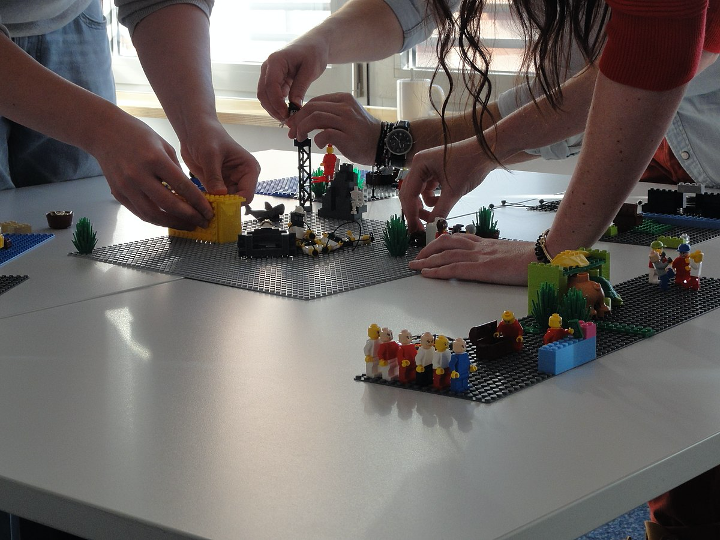
\includegraphics[scale=1.5]{Pictures/co-construccion.png}}} % Image background
%\AddToShipoutPicture*{\put(0,0){\includegraphics[height=900, width=650]{Pictures/exponential.png}}} % Image background
\centering
\vspace*{11.3cm}
\par\normalfont\fontsize{35}{35}\sffamily\selectfont

\begin{center}
    % List of Latex Colour names here: https://www.overleaf.com/learn/latex/Using_colours_in_LaTeX
    \textbf{\color{Orange} \mytitle}  % Modify the name of the colour used to suit your image
    
    %\textbf{\color{White}(\ILMCode)} % Modify the name of the colour used to suit your image
    
    %\color{black}ILM\par % Modify the name of the colour used to suit your image
  \end{center}

   \vspace*{5cm}
   \LARGE  \color{white} \textbf{\author \\ \id} % Modify the name of the colour used to suit your image

    %(\id)\par  


\endgroup

%----------------------------------------------------------------------------------------
%	COPYRIGHT PAGE
%----------------------------------------------------------------------------------------


\newpage
~\vfill
\thispagestyle{empty}


\noindent \textbf{Objetivo de este documento}
\vspace{0.5cm}

\noindent Este documento ha sido preparado para complementar lo visto en clases de Arquitectura de Sistemas de una manera que sea simple de seguir. Es un documento en evolución, por lo que sólo se permite el uso para los alumnos de la asignatura durante el tiempo que dure esta y se pide explícitamente no compartir en ningún medio. \\



\vspace{1cm}

%\noindent \textsc{\ILMCentreName - Report for the Award of a Level \ILMLevel Certificate from the Institute of Leadership and Management}\\

%\noindent This was written by \author, to be approved for submission by \reviewer. Written at the \ILMCentreName  (\ILMCentreCode).\\ % License information

\noindent Versión 0.1 - \textit{\date} % Printing/edition date

%----------------------------------------------------------------------------------------
%	TABLE OF CONTENTS
%----------------------------------------------------------------------------------------

\chapterimage{diferente2.png} % Table of contents heading image
\vspace{20px}
\pagestyle{empty} % No headers

\tableofcontents % Print the table of contents itself

%\listoftables %uncomment this if you want to print the list of tables at the start

\pagestyle{fancy} % Print headers again


%----------------------------------------------------------------------------------------
%	Glossary
%----------------------------------------------------------------------------------------

\chapterimage{Pictures/ampolletas.png} % Table of contents heading image
\vspace{20px}
\printglossaries
\chapterimage{../Pictures/iot.png}

\chapter{Repaso Express}
\vspace{160pt}

\section{Tomando los Requerimientos de la PuertaPerruna}

\begin{tcolorbox}[colback=gray!5!white,colframe=orange!60!gray,title=PuertaPerruna]
Los perros del siglo XXI también son independientes y el lema de esta empresa es "si se puede digitalizar/automatizar entonces digitalicémoslo/automaticémoslo". Como arquitecto de aplicaciones, apoyaremos en la prueba de concepto del sistema ciberfísico para la puerta perruna. La \textbf{PuertaPerruna} es un hardware de aproximadamente 40 cm de alto por 30 cm de ancho que se instala en la puerta de la casa y permite la salida y entrada del perro al patio a través de un sensor del ladrido. Si el sensor de ladrido reconoce el sonido del perro con el cual fue configurado, la puerta se activa y se abrirá o cerrará por un espacio de X segundos, teniendo un sensor de movimiento para evitar el cierre brusco y posible golpe al perro.
\end{tcolorbox}

\subsection{Requisitos Funcionales}
El sistema debe realizar las siguientes funciones:
\begin{itemize}
    \item RF1: \textbf{PuertaPerruna} deberá reconocer ladridos de perros registrados con una precisión superior al 98\%.
    \item RF2: \textbf{PuertaPerruna} deberá abrir la puerta.
    \item RF3: \textbf{PuertaPerruna} deberá cerrar la puerta.
    \item RF4: \textbf{PuertaPerruna} deberá determinar si es seguro cerrar.
    \item RF5: \textbf{PuertaPerruna} deberá saber siempre el estado de la puerta.
\end{itemize}

\subsection{Herramientas Utilizadas}
Para este caso utilizaremos las siguientes herramientas:
\begin{itemize}
    \item Python
    \item PlantUML
    \item VSCode
    \item Github
    \item copilot (opcional)
\end{itemize}

\begin{figure}[!h]
\centering
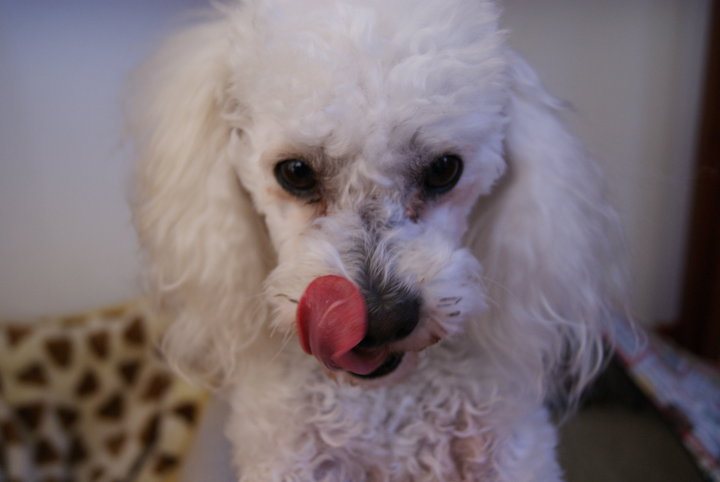
\includegraphics[scale=3]{Pictures/pompi.jpg}
\caption{Pompi, nuestro usuario de prueba para \textbf{PuertaPerruna} - un sistema que dará independencia a tus perros, y a ti, más horas de sueño.}
\label{fig:pompi}
\end{figure}

\subsection{Casos de Uso}
\subsubsection{Caso de Uso: Salir de Casa}
\begin{enumerate}
    \item \textbf{Actor}: El perro ladra dos veces frente a la puerta para poder salir.
    \item \textbf{Sistema}: El sensor de ladridos reconoce el ladrido del perro y envía la petición a la puerta para que se abra.
    \item \textbf{Sistema}: La puerta se abre.
    \item \textbf{Actor}: El perro sale.
    \item \textbf{Sistema}: La puerta espera X segundos y se cierra lentamente, volviéndose a abrir si detecta que aún hay movimiento y no es seguro cerrarse (reintentará cerrarse nuevamente luego de X segundos).
\end{enumerate}

\subsubsection{Caso de Uso: Entrar a Casa}
\begin{enumerate}
    \item \textbf{Actor}: El perro vuelve luego de hacer su negocio fuera de la casa y ladra para poder entrar.
    \item \textbf{Sistema}: El sensor de ladridos reconoce el ladrido del perro de la casa.
    \item \textbf{Sistema}: El sensor envía la petición a la puerta para que se abra.
    \item \textbf{Sistema}: La puerta se abre.
    \item \textbf{Actor}: El perro entra.
    \item \textbf{Sistema}: La puerta espera X segundos y se cierra lentamente, volviéndose a abrir si detecta que aún hay movimiento y no es seguro cerrarse (reintentará cerrarse nuevamente luego de X segundos).
\end{enumerate}

\begin{tcolorbox}[colback=gray!5!white,colframe=orange!60!gray,title=TODO]
Escribir a nivel de análisis el diagrama de secuencia para este flujo. Usar \url{https://pdf.plantuml.net/1.2021.1/PlantUML_Language_Reference_Guide_es.pdf}
\end{tcolorbox}

\subsection{Diagramas de Secuencia y Dominio}
\begin{tcolorbox}[colback=gray!5!white,colframe=orange!60!gray,title=Diagrama de Secuencia en PlantUML]
\begin{verbatim}
@startuml
actor Perro
participant "Sistema PuertaPerruna" as Sistema

Perro -> Sistema: Ladra para salir
Sistema -> Sistema: Detectar ladrido
Sistema -> Sistema: Abrir puerta
Sistema -> Perro: Puerta abierta
Perro -> Sistema: Sale
Sistema -> Sistema: Inicia temporizador para cerrar
Sistema -> Sistema: Detecta movimiento
Sistema -> Sistema: Cierra puerta si es seguro
@enduml
\end{verbatim}
\end{tcolorbox}

\begin{figure}[!h]
\centering
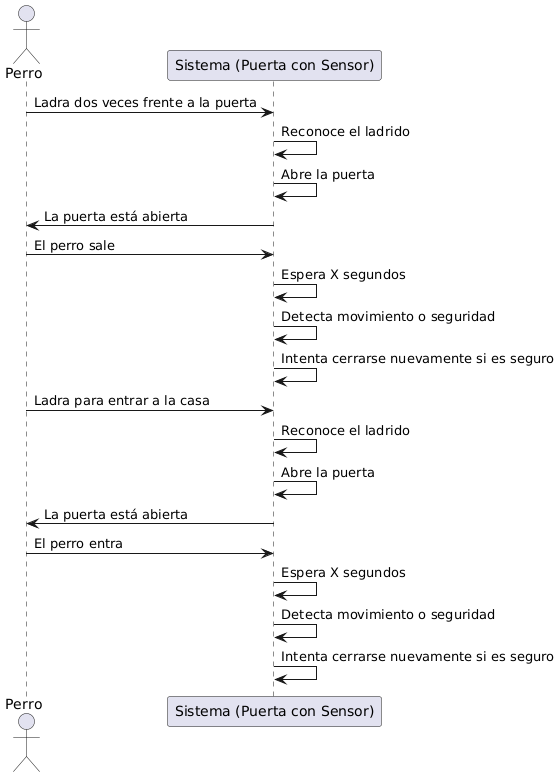
\includegraphics[scale=0.5]{Pictures/pp_analisis.png}
\caption{Diagrama a nivel de análisis.}
\label{fig:diag-sec}
\end{figure}

\begin{tcolorbox}[colback=gray!5!white,colframe=orange!60!gray,title=Modelo de Dominio en PlantUML]
\begin{verbatim}
@startuml
entity "Perro" as Perro {
    * nombre
    * raza
    * edad
}

entity "Puerta" as Puerta {
    * estado: {Abierta | Cerrada}
    * tiempo de cierre
}

entity "Sensor" as Sensor {
    * tipo: {Ladrido | Movimiento}
    * configurado: Boolean
}

Perro --|> Sensor : "Activa"
Sensor -- Puerta : "Controla"
@enduml
\end{verbatim}
\end{tcolorbox}

\begin{figure}[!h]
\centering
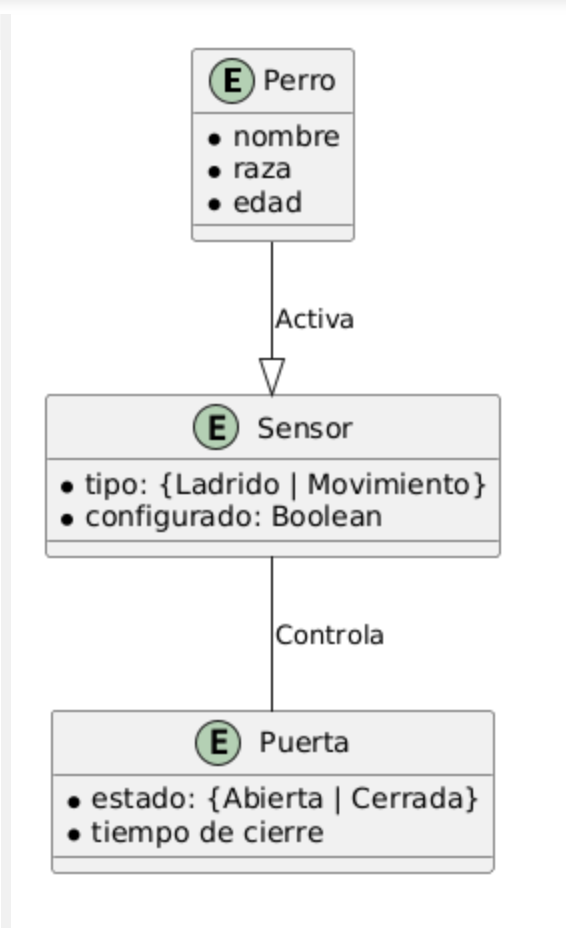
\includegraphics[scale=0.5]{Pictures/dominio.png}
\caption{Diagrama de dominio.}
\label{fig:diag-dom}
\end{figure}

\subsection{Diagrama de Estados}
El siguiente diagrama muestra los estados posibles de la \textbf{PuertaPerruna}:

\begin{tcolorbox}[colback=gray!5!white,colframe=orange!60!gray,title=Diagrama de Estados en PlantUML]
\begin{verbatim}
@startuml
[*] --> Cerrada
Cerrada --> Abierta: Detecta ladrido
Abierta --> Cerrada: Temporizador expira
Abierta --> Abierta: Detecta movimiento
Cerrada --> Cerrada: Sin eventos
@enduml
\end{verbatim}
\end{tcolorbox}

\begin{figure}[!h]
\centering
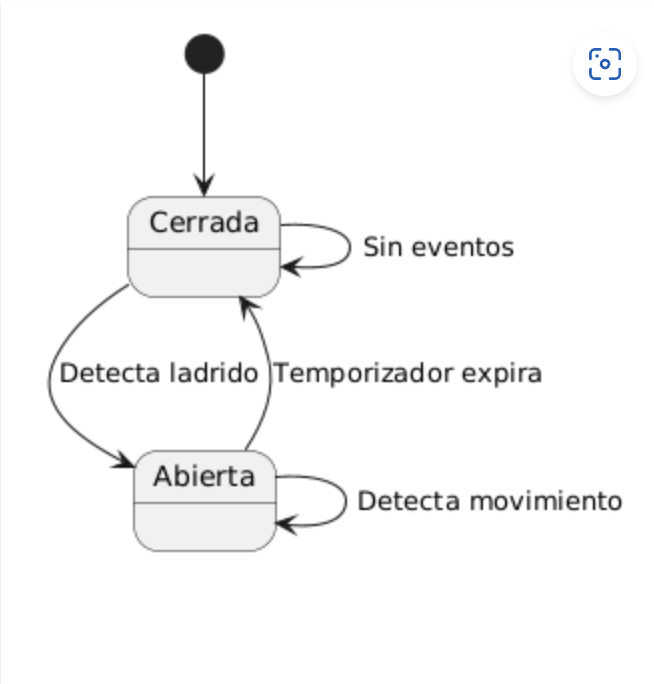
\includegraphics[scale=0.5]{Pictures/estados.png}
\caption{Diagrama de estado.}
\label{fig:diag-estado}
\end{figure}

\section*{Actividad: Preparación y Ejecución}

\subsection*{Parte 0: Tomar los Cursitos}
\begin{itemize}
    \item \url{https://github.com/skills/introduction-to-github}
    \item \url{https://github.com/skills/github-pages}
\end{itemize}

\subsection*{Parte 1: Creación del Repositorio}
Un integrante del equipo deberá:
\begin{enumerate}
    \item Crear un repositorio en GitHub con el nombre \texttt{PuertaPerruna}.
    \item Subir los archivos iniciales de código en Python.
    \item Compartir el enlace del repositorio con el equipo.
\end{enumerate}

\subsection*{Parte 2: Clonación y Ejecución}
Otro integrante deberá:
\begin{enumerate}
    \item Clonar el repositorio utilizando VSCode o el terminal con: \texttt{git clone <URL del repositorio>}.
    \item Ejecutar el archivo principal \texttt{simuladorBobby.py}.
    \item Comprobar el funcionamiento y realizar mejoras si es necesario.
\end{enumerate}

\subsection*{Parte 3: Adición de Casos de Prueba Unitaria usando IA Generativa}
\textbf{Objetivo:} Utilizar un chat de IA generativa para apoyar la creación de casos de prueba unitaria y ejecutarlos en Visual Studio Code (VSCode).

\textbf{Instrucciones:}
\begin{enumerate}
    \item \textbf{Preparación del Entorno:}
    \begin{itemize}
        \item Asegúrate de tener instalado VSCode y las extensiones necesarias para Python.
        \item Clona o descarga el código base proporcionado para la actividad.
    \end{itemize}
    
    \item \textbf{Uso de IA Generativa:}
    \begin{itemize}
        \item Utiliza un chat de IA generativa (como copilot integrado en VSCode) para obtener sugerencias sobre cómo escribir casos de prueba unitaria para el código base.
        \item Puedes formular preguntas específicas sobre cómo probar ciertas funciones o módulos del código.
    \end{itemize}
    
    \item \textbf{Escritura de Casos de Prueba:}
    \begin{itemize}
        \item Basándote en las sugerencias de la IA, escribe los casos de prueba unitaria en un archivo de prueba (por ejemplo, \texttt{test\_code.py}).
        \item Asegúrate de cubrir diferentes escenarios, incluyendo casos positivos y negativos.
    \end{itemize}
    
    \item \textbf{Ejecución de Pruebas:}
    \begin{itemize}
        \item Ejecuta los casos de prueba en VSCode utilizando una herramienta de pruebas como \texttt{unittest} o \texttt{pytest}.
        \item Verifica que todas las pruebas pasen y realiza ajustes en el código o en las pruebas según sea necesario.
    \end{itemize}
    
    \item \textbf{Documentación:}
    \begin{itemize}
        \item Documenta el proceso seguido, incluyendo las interacciones con la IA generativa y cómo estas ayudaron a mejorar los casos de prueba.
        \item Incluye cualquier desafío encontrado y cómo se resolvieron.
    \end{itemize}
\end{enumerate}

\subsection*{Parte 4: Uso de Git}
\textbf{Instrucciones:}
\begin{enumerate}
    \item Añade los archivos que deseas subir y realiza un commit:
    \begin{verbatim}
    git add .
    git commit -m "Añadir código de pruebas del sistema de puerta perruna"
    \end{verbatim}
    
    \item Sube los cambios al repositorio en GitHub:
    \begin{verbatim}
    git push origin master
    \end{verbatim}
    
    \item Estos comandos asumen que estás trabajando en la rama \texttt{master}. Si estás en otra rama, reemplaza \texttt{master} con el nombre de tu rama.
\end{enumerate}

\subsection*{Reflexión}
\begin{tcolorbox}[colback=gray!5!white,colframe=orange!60!gray,title=Preguntas]
\begin{itemize}
   \item \textbf{¿Qué importancia tiene ese diseño detallado?}
    - El diseño detallado es crucial porque actúa como un plano para el desarrollo del sistema. Ayuda a identificar posibles problemas antes de la implementación, facilita la comunicación entre los miembros del equipo y asegura que todos trabajen hacia un objetivo común.

\item \textbf{¿Qué técnicas se pueden utilizar para mantener el diseño y el código en sintonía durante todo el ciclo de vida del proyecto?}
    - Algunas técnicas incluyen el uso de herramientas de integración continua (CI) y entrega continua (CD), que permiten detectar y corregir desviaciones rápidamente. También es útil mantener una documentación actualizada y realizar reuniones de revisión de diseño periódicas.

\item \textbf{¿Cómo se puede verificar que el diseño detallado no se desvía de los requisitos iniciales del proyecto a medida que avanza?}
    - Se puede verificar mediante la realización de pruebas de aceptación basadas en los requisitos iniciales. Además, mantener una trazabilidad de los requisitos a lo largo del proyecto ayuda a asegurar que cada parte del diseño y la implementación se alinee con los objetivos originales.

\item \textbf{¿Qué herramientas y prácticas recomiendan para mantener la coherencia entre el diseño y la implementación del código?}
    - Herramientas como UML (Unified Modeling Language) para el diseño, junto con sistemas de control de versiones como Git, son muy útiles. Prácticas como el desarrollo basado en pruebas (TDD) y la revisión de código por pares también ayudan a mantener la coherencia entre el diseño y la implementación. 
\end{itemize}
\end{tcolorbox}

\chapterimage{Pictures/darwin.png}
\chapter{Introducción}
\vspace{140px}

\begin{flushright}
    \textit{Las ventajas de tener una buena arquitectura siempre debe ser satisfacer las necesidades de los stakeholders y entregar valor, además de su \underline{fácil integración}, \underline{flexibilidad}, su \underline{simple operación} y \underline{confiabilidad}. Todo sistema construido por el humano tiene una arquitectura la cual se define como una descripción abstracta de entidades de un sistema y sus relaciones, lo cual se traduce en un conjunto de decisiones que deben ser documentadas.}
\end{flushright}

\section{La Importancia de la Arquitectura de Sistemas}

La relevancia de una arquitectura de sistemas robusta se hace evidente cuando analizamos casos reales de la industria tecnológica moderna. Durante el primer Prime Day, Amazon experimentó un colapso debido a la alta demanda, un evento que subrayó la importancia de diseñar sistemas escalables. Este incidente no solo afectó las ventas inmediatas sino también la confianza de los usuarios y la reputación de la empresa. La respuesta de Amazon fue rediseñar su arquitectura para manejar peaks de carga extremos, implementando sistemas de auto-escalado y mejorando su infraestructura de manera significativa.

Netflix ofrece otro ejemplo ilustrativo de la importancia de la arquitectura de sistemas. En 2008, la compañía sufrió una interrupción importante en su centro de datos que afectó la distribución de DVDs durante tres días. Este incidente llevó a Netflix a repensar completamente su arquitectura, migrando a la nube y desarrollando herramientas como el "Chaos Monkey" para probar la resiliencia de sus sistemas. Hoy, Netflix puede transmitir contenido a más de 200 millones de suscriptores simultáneamente, un logro que sería imposible sin una arquitectura bien diseñada. Netflix utiliza microservicios y AWS para manejar su infraestructura, lo que permite una escalabilidad y resiliencia excepcionales. El uso de un API Gateway y servicios como Zuul facilita el enrutamiento dinámico y la seguridad, mientras que herramientas como Hystrix aseguran la resiliencia al aislar fallos.

Un sistema, en su esencia más fundamental, es más que la suma de sus partes. Cuando hablamos de sistemas, nos referimos a un conjunto de componentes que interactúan entre sí para servir a un propósito común. Esta interacción genera lo que llamamos "emergencia": comportamientos y propiedades que no existen en los componentes individuales, sino que surgen de su interacción. Por ejemplo, la capacidad de Google para procesar miles de millones de búsquedas diarias no es una propiedad de ningún servidor individual, sino que emerge de la interacción coordinada de múltiples centros de datos y sistemas distribuidos. La emergencia se refiere a lo que aparece o emerge cuando un sistema opera, es decir, su funcionalidad. Las funciones emergen de las interacciones entre los componentes del sistema, como se observa en sistemas complejos como los automóviles, donde funciones deseables y no deseables pueden surgir inesperadamente.

La arquitectura de sistemas moderna debe considerar aspectos que van más allá de la funcionalidad básica. En el sector financiero, por ejemplo, los sistemas deben mantener una disponibilidad cercana al 100\% mientras procesan millones de transacciones por segundo. El sistema SWIFT, que maneja la mayoría de las transferencias internacionales, procesa más de 42 millones de mensajes diarios, requiriendo una arquitectura que garantice no solo el rendimiento, sino también la seguridad y la trazabilidad de cada transacción.

En el sector salud, la arquitectura de sistemas enfrenta desafíos únicos. Los sistemas deben manejar datos sensibles de pacientes, cumplir con regulaciones estrictas como HIPAA, y estar disponibles en situaciones de emergencia. El caso del NHS (National Health Service) en Reino Unido durante el ataque de ransomware WannaCry en 2017 demostró cómo una arquitectura vulnerable puede poner en riesgo vidas humanas. Este incidente llevó a una reevaluación completa de la arquitectura de sistemas de salud a nivel nacional.

La emergencia en sistemas complejos puede manifestarse de formas inesperadas. Durante la crisis financiera de 2008, los sistemas automatizados de trading contribuyeron a una espiral de ventas que amplificó la volatilidad del mercado. Este ejemplo muestra cómo la interacción entre sistemas aparentemente bien diseñados puede generar comportamientos emergentes no deseados a escala sistémica. Como resultado, las arquitecturas modernas de sistemas financieros ahora incluyen "circuit breakers" y otros mecanismos de control para prevenir tales escenarios.

\section{Fundamentos de Arquitectura de Sistemas}

Un sistema es un conjunto de entidades y sus relaciones, cuya funcionalidad es mayor que la suma de las partes. Esta definición fundamental nos ayuda a entender que un producto no necesariamente es un sistema (e.g.: pasta) y un sistema no siempre es un producto (e.g.: sistema solar). Las funciones son lo que el sistema hace: sus acciones y salidas, y estas funciones emergen de las interacciones entre los componentes del sistema. La descomposición de un sistema complejo, como un smartphone, en subsistemas y componentes, es esencial para mostrar la importancia de la modularidad. Cada subsistema debe integrarse con otros para formar un sistema cohesivo, permitiendo una mejor gestión y evolución del sistema.

\section{Roles en la Arquitectura}

En el contexto empresarial, las organizaciones se dividen en divisiones, departamentos y equipos que poseen diferentes roles y responsabilidades, lo que resulta en una arquitectura empresarial compleja. En este ecosistema, podemos identificar dos roles fundamentales:

\subsection{El Arquitecto Empresarial}
Los arquitectos empresariales no controlan la funcionalidad de ninguna aplicación específica, sino que diseñan el ecosistema dentro del cual las aplicaciones individuales contribuyen a la empresa como un todo. Su rol es crucial para permitir que la empresa cumpla sus metas estratégicas, estableciendo restricciones y lineamientos para los arquitectos de aplicaciones.

\subsection{El Arquitecto de Aplicaciones}
Un arquitecto de aplicaciones es un desarrollador responsable de una aplicación particular. Estos profesionales entienden y administran los miles de objetos que comprenden la aplicación y con sus acciones diarias van formando el producto final.

\begin{remark}
\textit{Realizando una analogía con la industria cinematográfica, el arquitecto empresarial es como el productor y los arquitectos de aplicaciones son los directores}.
\end{remark}

\section{La Importancia de la Estandarización}

La separación entre arquitecto empresarial y arquitecto de aplicaciones ayuda a la compañía a evitar la heterogeneidad y prevenir el caos. Esta estructura busca la \textit{estandarización} y el orden. Por tanto, es fundamental que todo desarrollador dentro de la organización:
\begin{itemize}
    \item Entienda los principios claves de la arquitectura empresarial
    \item Comprenda las restricciones establecidas
    \item Reconozca cómo sus objetivos y metas en cada \textbf{propiedad de calidad} contribuyen a la arquitectura empresarial global
\end{itemize}

Las normas ISO/IEC/IEEE y organizaciones como IETF, OMG y W3C juegan un papel crucial en la estandarización de la arquitectura de sistemas. Estas normas aseguran que las arquitecturas sean consistentes, interoperables y seguras, facilitando la colaboración y la innovación a nivel global.

\section{Arquitectura en el Contexto Ágil}

Desarrollar software para grandes organizaciones impone desafíos significativos. El desarrollo de software ágil surgió como una reacción a los procesos de desarrollo ``pesados'', enfatizando la construcción eficiente de productos que los clientes realmente necesitan. Para 2008, el 69\% de las compañías habían implementado metodologías ágiles en al menos uno de sus proyectos.

Sin embargo, existe un debate sobre el rol de la arquitectura en el desarrollo ágil. Mientras algunos desarrolladores ágiles sugieren minimizar las técnicas de arquitectura de software, expertos como Martin Fowler defienden su importancia. El \textbf{refactoring} en sistemas grandes y legados, aunque costoso, puede ser necesario para mantener la calidad del sistema.

\section{Arquitectura Suficiente}

Es crucial determinar cuánta arquitectura es suficiente. Una arquitectura adecuada debe permitir que diferentes stakeholders:
\begin{itemize}
    \item Entiendan su integración con los procesos organizacionales
    \item Comprendan los servicios que el sistema proporcionará
    \item Identifiquen los bloques de construcción básicos
    \item Entiendan los requerimientos de despliegue y niveles de servicio
    \item Mantengan el código según las decisiones de diseño establecidas
\end{itemize}

El modelo de arquitectura dirigido por riesgo guía a los desarrolladores a implementar la arquitectura suficiente para alcanzar sistemas \textit{seguros}, \textit{escalables} y \textit{altamente disponibles}.

\begin{figure}
    \centering
    
\includegraphics{Pictures/elarquitecto.png}
    \caption{Fuente externa: Película Matrix}
    \label{fig:arq}
\end{figure}

\section{Del Desarrollo Individual a la Ingeniería de Software a Gran Escala}

El desarrollo de software ha experimentado una transformación radical desde sus inicios en los años 50. Lo que comenzó con programadores individuales escribiendo código en tarjetas perforadas ha evolucionado hasta convertirse en una disciplina compleja que involucra equipos distribuidos globalmente. Esta evolución no ha sido solo en escala, sino también en complejidad y metodología. El pensamiento sistémico es crucial en este contexto, ya que permite ver un sistema como un conjunto de entidades interrelacionadas cuya funcionalidad es mayor que la suma de las entidades individuales. Este enfoque ayuda a comprender y diseñar sistemas complejos, asegurando que todas las implicaciones importantes de las decisiones sean consideradas.

Consideremos la evolución de un caso típico: un sistema de reservas hoteleras. En sus inicios, un pequeño equipo podría desarrollar una aplicación para un hotel local, manejando reservaciones, check-in/check-out y facturación básica. Sin embargo, cuando este mismo sistema necesita escalar para servir a una cadena hotelera internacional, surgen desafíos completamente nuevos: manejo de diferentes monedas, regulaciones locales variables, múltiples zonas horarias, y picos de demanda que varían según la región y temporada.

La complejidad de los sistemas modernos se ilustra perfectamente en el sector bancario. En la década de 1970, un banco típico podría operar con un mainframe central y terminales simples. Hoy, un banco digital como Nubank en Brasil debe gestionar más de 70 millones de clientes a través de múltiples servicios interconectados: cuentas corrientes, tarjetas de crédito, inversiones, seguros y préstamos. Cada uno de estos servicios podría considerarse una aplicación compleja por sí misma, pero deben funcionar como un ecosistema cohesivo.

El caso de Spotify ilustra cómo la arquitectura debe evolucionar con el crecimiento. Comenzaron con una arquitectura monolítica tradicional, pero a medida que su base de usuarios creció a cientos de millones, tuvieron que adoptar una arquitectura de microservicios. Este cambio no fue solo técnico; requirió reorganizar equipos completos alrededor del concepto de "squads" y "tribes", demostrando cómo la arquitectura del sistema influye en la estructura organizacional y viceversa (Ley de Conway).

La Ingeniería de Software a Gran Escala (VLSE) introduce desafíos que van más allá del código. Cuando Google decide actualizar su algoritmo de búsqueda, el cambio debe probarse y desplegarse en miles de servidores sin interrumpir el servicio. Esto requiere no solo excelencia técnica, sino también procesos sofisticados de desarrollo, prueba y despliegue. Google desarrolló herramientas como Bazel y Monarch específicamente para manejar la escala de su operación.

La modularidad se convierte en un principio fundamental en VLSE, pero su implementación efectiva es más compleja de lo que parece. PayPal aprendió esta lección cuando intentó modernizar su arquitectura heredada. En lugar de realizar una reescritura completa (que había fallado anteriormente), adoptaron un enfoque gradual de "strangler fig pattern", donde los nuevos servicios modulares fueron reemplazando gradualmente al sistema antiguo. Este proceso tomó años, pero permitió mantener la operación continua mientras se modernizaba la arquitectura.

Los sistemas a gran escala también deben manejar fallos de manera diferente. Netflix, por ejemplo, opera bajo el principio de "diseño para el fallo". Su arquitectura asume que los componentes fallarán y está diseñada para degradarse elegantemente. Cuando un servicio de recomendaciones falla, el sistema puede seguir transmitiendo contenido, aunque sin recomendaciones personalizadas. Este enfoque de "degradación elegante" es fundamental en sistemas que deben mantener alta disponibilidad.

La seguridad en VLSE presenta sus propios desafíos únicos. El ataque a Target en 2013, donde se comprometieron 40 millones de tarjetas de crédito, comenzó a través de un proveedor de HVAC con acceso a la red corporativa. Este incidente demostró cómo en sistemas grandes, la superficie de ataque se expande más allá de los límites tradicionales del sistema, requiriendo un enfoque holístico de la seguridad.

La integración de sistemas es fundamental para conectar diferentes componentes, destacando la flexibilidad y la estandarización. El uso de middleware permite que los sistemas se comuniquen de manera eficiente, facilitando la interoperabilidad y la cohesión. 

Un ejemplo puntual de integración de sistemas es el de las ciudades inteligentes. En una ciudad inteligente, múltiples subsistemas como el tráfico, la gestión de residuos, la energía y la seguridad deben trabajar juntos de manera cohesiva. Por ejemplo, los sensores de tráfico pueden enviar datos en tiempo real a un sistema central que ajusta los semáforos para optimizar el flujo vehicular. Este sistema central puede estar integrado con aplicaciones móviles que informan a los ciudadanos sobre las condiciones del tráfico, reduciendo así los tiempos de viaje y mejorando la eficiencia del transporte público.

Otro caso notable es el gobierno digital en Estonia. Estonia ha implementado un sistema de gobierno digital que permite a los ciudadanos realizar casi todas las interacciones gubernamentales en línea, desde votar hasta pagar impuestos. Este sistema se basa en la integración de múltiples subsistemas, como el registro civil, la seguridad social y los servicios de salud. Por ejemplo, cuando un niño nace, el hospital registra el nacimiento en el sistema digital, que automáticamente actualiza el registro civil, emite un número de identificación personal y notifica a los servicios de salud y seguridad social. Esta integración reduce la burocracia, mejora la eficiencia y proporciona un servicio más rápido y preciso a los ciudadanos.

Estos ejemplos muestran cómo la integración de sistemas, facilitada por el uso de middleware, puede mejorar significativamente la eficiencia y la calidad de los servicios en diferentes contextos.

\section{Desafíos Actuales y Futuros}

Los sistemas heredados representan uno de los mayores desafíos en la arquitectura moderna, un problema que se vuelve más crítico con el paso del tiempo. El caso de HSBC en 2015, donde problemas con un sistema COBOL de 30 años afectaron los pagos de nómina, es apenas la punta del iceberg. En el sector financiero, se estima que el 43\% de los sistemas bancarios centrales todavía funcionan en COBOL, procesando diariamente millones de transacciones valoradas en billones de dólares. La modernización de estos sistemas no es solo una cuestión de actualizar tecnología, sino de mantener la continuidad del negocio mientras se evoluciona.

La integración de la Inteligencia Artificial está transformando fundamentalmente la arquitectura de sistemas. Tesla, por ejemplo, no solo debe gestionar la operación de sus vehículos eléctricos, sino también manejar el entrenamiento continuo de sus modelos de IA con datos recopilados de millones de millas de conducción autónoma. Esto requiere una arquitectura que pueda manejar enormes volúmenes de datos en tiempo real, mientras mantiene la seguridad y confiabilidad necesarias para sistemas que involucran la seguridad humana.

El surgimiento de arquitecturas descentralizadas presenta nuevos desafíos y oportunidades. La adopción de blockchain en sistemas empresariales, como el proyecto Food Trust de IBM, que rastrea la cadena de suministro de alimentos, requiere repensar conceptos fundamentales de arquitectura. La inmutabilidad, la transparencia y la descentralización introducen nuevas consideraciones en el diseño de sistemas que tradicionalmente se basaban en bases de datos centralizadas y control jerárquico.

La seguridad y la privacidad se han convertido en preocupaciones centrales en la arquitectura moderna. El caso de Cambridge Analytica y Facebook demostró cómo las decisiones arquitectónicas pueden tener ramificaciones que van más allá de lo técnico, afectando la privacidad de millones de usuarios y potencialmente influenciando procesos democráticos. Las arquitecturas modernas deben incorporar principios de "privacidad por diseño" y considerar las implicaciones éticas de sus decisiones técnicas.

El edge computing está redefiniendo dónde y cómo se procesan los datos. Organizaciones como Cloudflare están construyendo redes de edge computing que permiten procesar datos más cerca de donde se generan, reduciendo la latencia y mejorando la experiencia del usuario. Sin embargo, esto introduce nuevos desafíos en términos de consistencia de datos, seguridad y mantenimiento de sistemas distribuidos a escala global.

La sostenibilidad emerge como una nueva dimensión en la arquitectura de sistemas. Google, por ejemplo, ha rediseñado sus centros de datos para optimizar la eficiencia energética, utilizando IA para reducir el consumo de energía en refrigeración en un 40\%. Las arquitecturas futuras deberán considerar su impacto ambiental como un requisito no funcional crítico.

El desarrollo ágil continúa desafiando las prácticas tradicionales de arquitectura. Aunque algunos desarrolladores ágiles sugieren minimizar el enfoque en la arquitectura, la experiencia ha demostrado que la agilidad y la buena arquitectura no son mutuamente excluyentes. Spotify, por ejemplo, ha demostrado cómo una arquitectura bien pensada puede facilitar la entrega continua y la innovación rápida, mientras mantiene la estabilidad del sistema.

La gestión de la complejidad sigue siendo un desafío fundamental. Los sistemas modernos deben integrar múltiples tecnologías, frameworks y plataformas, cada una con su propia curva de aprendizaje y peculiaridades. Amazon, por ejemplo, utiliza más de 100 servicios diferentes en su plataforma de comercio electrónico. Mantener esta complejidad manejable requiere un equilibrio cuidadoso entre la innovación y la estandarización.

Mirando hacia el futuro, la computación cuántica podría revolucionar completamente nuestro enfoque de la arquitectura de sistemas. IBM y Google están desarrollando computadoras cuánticas que podrían resolver ciertos problemas exponencialmente más rápido que las computadoras clásicas. Esto podría requerir una reconsideración fundamental de cómo diseñamos y optimizamos nuestros sistemas.

La arquitectura de sistemas está en constante evolución, impulsada por nuevas tecnologías, requisitos cambiantes y lecciones aprendidas de éxitos y fracasos pasados. El desafío para los arquitectos modernos es mantener sistemas que sean lo suficientemente robustos para ser confiables, lo suficientemente flexibles para evolucionar, y lo suficientemente simples para ser mantenidos efectivamente.



\chapterimage{map.png}

\chapter{Arquitectura Empresarial}

\section{Fundamentos de Arquitectura Empresarial}

\subsection{Definición y Propósito}

La Arquitectura Empresarial (AE) es un conjunto integrado de elementos que se utilizan en el diseño y realización de la estructura organizativa, los procesos de negocio, los sistemas de información y la infraestructura de una empresa. Es una práctica estratégica que ayuda a las organizaciones a alinear sus recursos tecnológicos con sus objetivos de negocio.

La AE proporciona:
\begin{itemize}
\item Una visión holística de la organización
\item Un marco para la toma de decisiones estratégicas
\item Una base para la transformación digital
\item Un puente entre la estrategia empresarial y su ejecución
\end{itemize}

\subsection{Beneficios de la Arquitectura Empresarial}

La implementación de una AE ofrece múltiples beneficios:

\begin{itemize}
\item \textbf{Visión común:} Proporciona una visión común de la organización.
\item \textbf{Reducción de complejidad:} Facilita la evolución de los sistemas de información.
\item \textbf{Optimización de costos:} Reduce costos removiendo redundancias.
\item \textbf{Gestión de riesgos:} Reduce riesgos tecnológicos.
\item \textbf{Mejora colaborativa:} Facilita la colaboración entre equipos.
\item \textbf{Alineación estratégica:} Alinea inversiones con objetivos.
\item \textbf{Cumplimiento normativo:} Facilita el cumplimiento regulatorio.
\item \textbf{Resiliencia:} Crea resiliencia organizacional.
\item \textbf{Interoperabilidad:} Garantiza la interoperabilidad del sistema.
\item \textbf{Estandarización:} Estandariza prácticas y procesos.
\end{itemize}



\section{Modelado con ArchiMate}

ArchiMate es el lenguaje de modelado estándar para arquitectura empresarial. Proporciona una forma consistente de visualizar y describir arquitecturas empresariales.

\subsection{Elementos Básicos de ArchiMate}

ArchiMate organiza sus elementos en tres capas principales:
\begin{itemize}
\item \textbf{Capa de Negocio:} Servicios, procesos y actores de negocio
\item \textbf{Capa de Aplicación:} Servicios y componentes de aplicación
\item \textbf{Capa de Tecnología:} Infraestructura y plataformas
\end{itemize}

\subsection{Vistas y Viewpoints}

ArchiMate permite crear diferentes vistas según las necesidades:
\begin{itemize}
\item Vista de Organización
\item Vista de Procesos
\item Vista de Información
\item Vista de Aplicaciones
\item Vista de Infraestructura
\item Vista de Implementación
\end{itemize}

\section{Evaluación de Arquitecturas Empresariales}

La evaluación de arquitecturas empresariales se realiza considerando múltiples dimensiones:

\subsection{Criterios de Evaluación}
\begin{itemize}
\item \textbf{Alineación Estratégica:} ¿La arquitectura soporta los objetivos del negocio?
\item \textbf{Valor del Negocio:} ¿Genera beneficios tangibles?
\item \textbf{Riesgos:} ¿Los riesgos están identificados y gestionados?
\item \textbf{Viabilidad:} ¿Es factible implementar la arquitectura?
\item \textbf{Sostenibilidad:} ¿La arquitectura es mantenible a largo plazo?
\end{itemize}

\subsection{Métricas de Evaluación}
\begin{itemize}
\item Retorno sobre la Inversión (ROI)
\item Tiempo de implementación
\item Costos operativos
\item Nivel de satisfacción de usuarios
\item Cumplimiento regulatorio
\end{itemize}

\section{Caso Práctico: Archisurance}

Manual archi \url{https://www.archimatetool.com/downloads/archi/Archi%20User%20Guide.pdf} 
\\ Caso Archisurance completo \url{https://github.com/archimate-models/archisurance} \\

\begin{tcolorbox}[colback=gray!5!white,colframe=orange!60!gray,title=Archisurance]
Tres compañías de seguros (autos, viajes/casa, legal) ubicadas en diferentes regiones del país, con una buena cartera de clientes, con modelos de negocios similares(seguros), con canales de ventas similares (mediante web, Teléfono y medios postales) han decidido fusionarse. Las razones (drivers) son principalmente pues esto les podría permitir disminuir los costos cuando entran a nuevos mercados, nuevas oportunidades de crecer en otras regiones y la inversión que requieren en TI para mantenerse competitivas puede ser compartido.
\end{tcolorbox}

\subsection{Desarrollo del Caso con Archi}

Para modelar este caso utilizaremos Archi, una herramienta de código abierto para ArchiMate. El proceso incluye:

\subsubsection{Paso 1: Identificación de Stakeholders}
\begin{itemize}
\item Crear nuevo modelo en Archi
\item Identificar stakeholders principales
\item Documentar sus preocupaciones
\end{itemize}

\subsubsection{Paso 2: Análisis de Motivación}
\begin{itemize}
\item Crear vista de motivación
\item Identificar drivers del negocio
\item Establecer metas y objetivos
\end{itemize}

\begin{figure}[h]
\centering
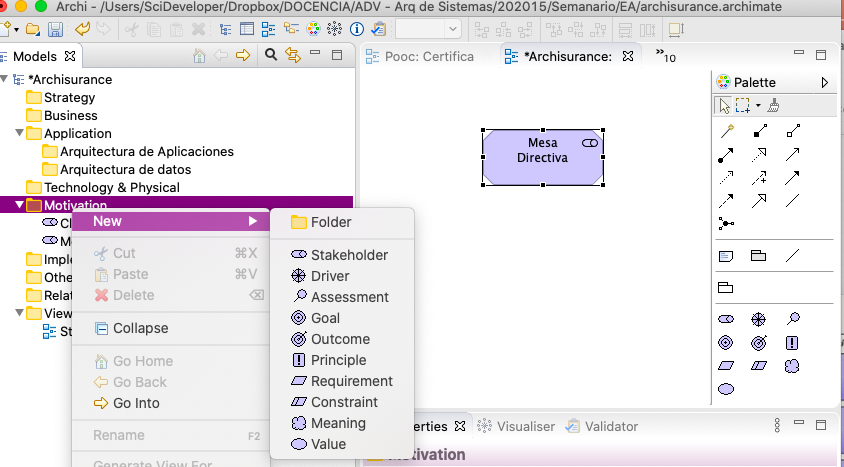
\includegraphics[scale=0.35]{Pictures/addstake.png}
\caption{Agregando stakeholders en Archi.}
\label{fig:stakeholders}
\end{figure}

\subsubsection{Paso 3: Modelado de Arquitectura}
\begin{itemize}
\item Desarrollar vista de negocio
\item Crear vista de aplicaciones
\item Diseñar vista de tecnología
\end{itemize}

\begin{figure}[h]
\centering
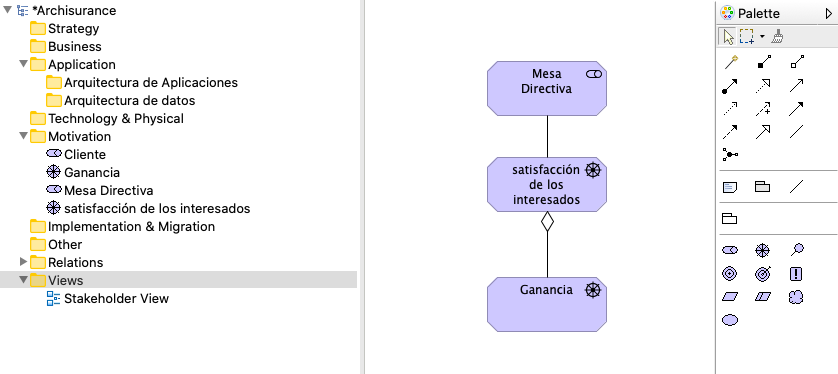
\includegraphics[scale=0.35]{Pictures/jeraquiadrivers.png}
\caption{Jerarquía de drivers en Archi.}
\label{fig:drivers}
\end{figure}




\section{Marco de Referencia TOGAF}

\subsection{Introducción a TOGAF}

The Open Group Architecture Framework (TOGAF) es un marco reconocido globalmente para el desarrollo y la gestión de arquitecturas empresariales. Diseñado para arquitectos empresariales y responsables de arquitectura en organizaciones, TOGAF ofrece un enfoque estructurado y flexible.

Inicialmente desarrollado en 1995, basado en el Marco de Arquitectura Técnica para la Gestión de la Información (TAFIM) del Departamento de Defensa de los Estados Unidos, TOGAF ha evolucionado para adaptarse a las necesidades modernas. Permite a las organizaciones optimizar su estructura para responder al cambio y respaldar estrategias empresariales.

\begin{figure}[h]
\centering
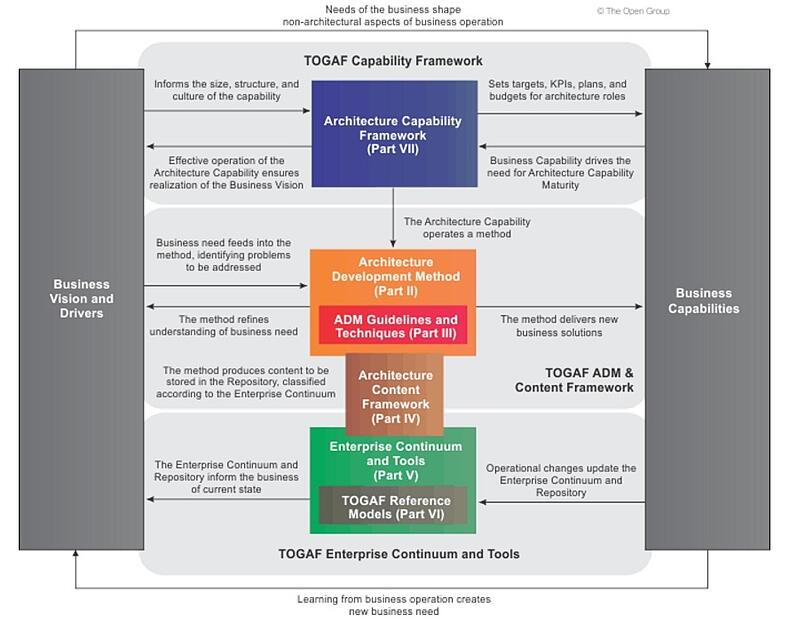
\includegraphics[scale=0.6]{Pictures/togaf.jpg}
\caption{Estructura del estándar TOGAF.}
\label{fig:togaf_structure}
\end{figure}

\subsection{Dominios de la Arquitectura Empresarial}

La AE se divide en cuatro dominios principales que trabajan de manera integrada:

\subsubsection{Arquitectura de Negocio}
Define la estrategia del negocio, la gobernanza, la estructura y los procesos clave. Incluye:
\begin{itemize}
\item Procesos de negocio
\item Estructura organizacional
\item Objetivos y metas estratégicas
\item Servicios de negocio
\item Métricas de rendimiento
\end{itemize}

\subsubsection{Arquitectura de Datos}
Describe la estructura de los datos lógicos y físicos de la organización:
\begin{itemize}
\item Modelos de datos
\item Políticas de gestión de datos
\item Estándares de datos
\item Flujos de información
\item Calidad y gobierno de datos
\end{itemize}

\subsubsection{Arquitectura de Aplicaciones}
Define las aplicaciones necesarias para procesar los datos y soportar las funciones del negocio:
\begin{itemize}
\item Catálogo de aplicaciones
\item Interfaces entre aplicaciones
\item Ciclos de vida de las aplicaciones
\item Patrones de arquitectura
\item Integración de sistemas
\end{itemize}

\subsubsection{Arquitectura Tecnológica}
Describe la infraestructura de hardware y software que soporta las aplicaciones y datos:
\begin{itemize}
\item Infraestructura de TI
\item Redes y comunicaciones
\item Procesamiento y almacenamiento
\item Estándares tecnológicos
\item Seguridad tecnológica
\end{itemize}

\section{Método de Desarrollo de Arquitectura (ADM)}

El ADM de TOGAF es un método iterativo que guía el desarrollo de la arquitectura empresarial a través de un ciclo continuo de definición y realización de arquitectura.

\subsection{Fases del ADM}
\begin{itemize}
\item \textbf{Fase Preliminar:} Preparación e iniciación. Establece las capacidades arquitectónicas iniciales.
\item \textbf{Fase A:} Visión de Arquitectura. Define el alcance, limitaciones y expectativas del proyecto arquitectónico.
\item \textbf{Fase B:} Arquitectura de Negocio. Desarrolla la arquitectura de negocio para apoyar la visión acordada.
\item \textbf{Fase C:} Arquitectura de Sistemas de Información. Desarrolla las arquitecturas de datos y aplicaciones.
\item \textbf{Fase D:} Arquitectura Tecnológica. Define la infraestructura necesaria para soportar la arquitectura objetivo.
\item \textbf{Fase E:} Oportunidades y Soluciones. Identifica los principales proyectos de implementación.
\item \textbf{Fase F:} Planificación de Migración. Desarrolla el plan detallado de implementación y migración.
\item \textbf{Fase G:} Gobierno de Implementación. Supervisa la implementación para asegurar conformidad.
\item \textbf{Fase H:} Gestión de Cambios en la Arquitectura. Monitorea y gestiona los cambios.
\end{itemize}

\subsection{Componentes Clave del ADM}
\begin{itemize}
\item \textbf{Entregables:} Son los productos de trabajo formalmente revisados, acordados y firmados por los stakeholders. Incluyen:
  \begin{itemize}
    \item Documentos de definición de arquitectura
    \item Especificaciones de requerimientos
    \item Planes de implementación y migración
    \item Evaluaciones de cumplimiento
  \end{itemize}

\item \textbf{Artefactos:} Son los productos de trabajo específicos que describen un aspecto de la arquitectura:
  \begin{itemize}
    \item Catálogos: Listas de bloques de construcción
    \item Matrices: Muestran relaciones entre componentes
    \item Diagramas: Representaciones gráficas de la arquitectura
  \end{itemize}

\item \textbf{Bloques de Construcción:} Representan componentes reutilizables que:
  \begin{itemize}
    \item Pueden ser combinados para entregar arquitecturas y soluciones
    \item Proporcionan capacidades que resuelven necesidades del negocio
    \item Son reutilizables y configurables según el contexto
  \end{itemize}
\end{itemize}

\subsection{Aplicación del ADM: Caso DART-MINSAL}

Para ilustrar la aplicación práctica del ADM, analizaremos el caso del sistema DART (Detección Automatizada de Retinopatía Diabética) del MINSAL:

\subsubsection{Fase Preliminar}
\begin{itemize}
\item \textbf{Contexto:} Sistema de salud chileno con déficit de 39,168 horas de atención oftalmológica
\item \textbf{Principios:} 
  \begin{itemize}
    \item Acceso equitativo a servicios de salud
    \item Optimización de recursos médicos
    \item Transformación digital en salud pública
  \end{itemize}
\end{itemize}

\subsubsection{Fase A: Visión de Arquitectura}
\begin{itemize}
\item \textbf{Objetivos Estratégicos:}
  \begin{itemize}
    \item Reducir tiempo de diagnóstico de 30 a 5 días
    \item Optimizar uso de oftalmólogos (de 39,168 a 15,000 horas/año)
    \item Aumentar cobertura en zonas rurales de 40\% a 90\%
  \end{itemize}
\item \textbf{Balance Scorecard:}
  \begin{itemize}
    \item Perspectiva Financiera: Reducción de costos en diagnósticos
    \item Perspectiva Cliente: Garantizar acceso oportuno a servicios
    \item Perspectiva Procesos: Reducir brechas en zonas rurales
    \item Perspectiva Aprendizaje: Prevenir enfermedades crónicas
  \end{itemize}
\end{itemize}

\subsubsection{Fase B: Arquitectura de Negocio}
\begin{itemize}
\item \textbf{Procesos Clave:}
  \begin{itemize}
    \item Preprocesar imágenes
    \item Detectar signos de retinopatía
    \item Generar propuesta de reporte
    \item Validación profesional
    \item Notificar paciente
  \end{itemize}
\item \textbf{Actores:} MinSal, Oftalmólogos, Pacientes diabéticos
\end{itemize}

\subsubsection{Fase C: Arquitectura de Sistemas de Información}
\begin{itemize}
\item \textbf{Arquitectura de Datos:}
  \begin{itemize}
    \item Datos de Ficha Clínica
    \item Imágenes de Retina
    \item Datos de Informes Médicos
  \end{itemize}
\item \textbf{Arquitectura de Aplicaciones:}
  \begin{itemize}
    \item DART Connector
    \item CRM
    \item Notifier
    \item DataTransformer
  \end{itemize}
\end{itemize}

\subsubsection{Fase D: Arquitectura Tecnológica}
\begin{itemize}
\item \textbf{Infraestructura Hospital:}
  \begin{itemize}
    \item Servidor de Telemedicina
    \item Servidor de Imagenología
    \item Conector DART
  \end{itemize}
\item \textbf{Infraestructura Nube:}
  \begin{itemize}
    \item Servidor de Procesamiento IA
    \item Repositorio de Diagnósticos
    \item API Gateway del MINSAL
  \end{itemize}
\item \textbf{Seguridad:}
  \begin{itemize}
    \item Cifrado de datos
    \item VPN/Canales Seguros
    \item Autenticación entre sistemas
  \end{itemize}
\end{itemize}

\subsubsection{Fase E: Oportunidades y Soluciones}
\begin{itemize}
\item \textbf{Proyectos Identificados:}
  \begin{itemize}
    \item Implementación de DART en hospitales
    \item Automatización del cribado con IA
    \item Expansión de estaciones de diagnóstico
    \item Integración con ficha clínica electrónica
  \end{itemize}
\end{itemize}

\subsubsection{Fase F: Plan de Migración}
\begin{itemize}
\item \textbf{Métricas Clave:}
  \begin{itemize}
    \item Tiempo promedio de diagnóstico
    \item Horas oftalmológicas utilizadas
    \item Cobertura de exámenes en APS rurales
    \item Nivel de digitalización de procesos
  \end{itemize}
\item \textbf{Metas a 5 Años:}
  \begin{itemize}
    \item Reducir tiempo de diagnóstico a 5 días
    \item Optimizar a 15,000 horas/año de oftalmólogos
    \item Alcanzar 90\% de cobertura rural
    \item Lograr 95\% de digitalización
  \end{itemize}
\end{itemize}

\begin{figure}[h]
\centering
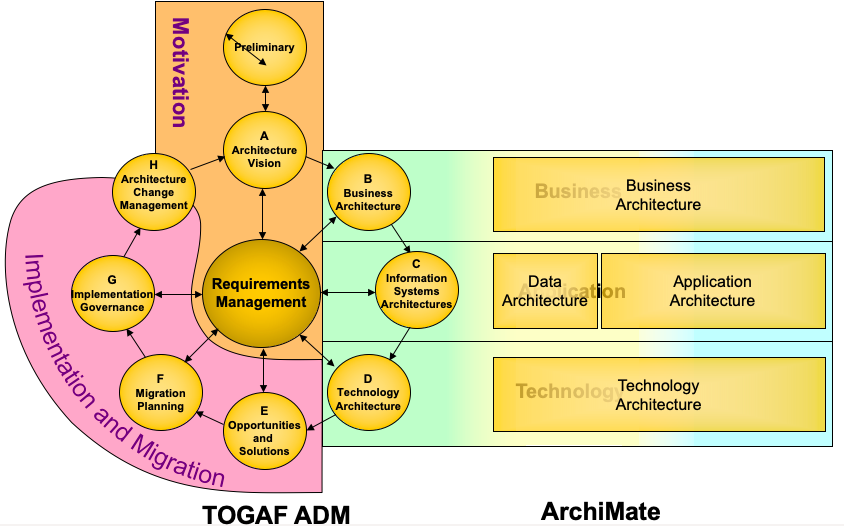
\includegraphics[scale=0.6]{Pictures/ADM.png}
\caption{Ciclo del Método de Desarrollo de Arquitectura (ADM).}
\label{fig:adm_phases}
\end{figure}




\section{Recursos y Referencias}

Para profundizar en el uso de Archi y ArchiMate:

\begin{itemize}
\item Manual Archi: \url{https://www.archimatetool.com/downloads/Archi\%20User\%20Guide.pdf}
\item Especificación ArchiMate: \url{https://pubs.opengroup.org/architecture/archimate3-doc/toc.html}
\item Caso Archisurance completo: \url{https://publications.opengroup.org/y163}
\end{itemize}




\chapterimage{map.png}

\chapter{Arquitectura de Software}


\section{Fundamentos del Diseño Arquitectónico}

El diseño de arquitectura de software es la base fundamental para cualquier sistema de software complejo. Desafortunadamente, con frecuencia se realiza de manera ad hoc, si es que se realiza. Es nuestra convicción, basada en la experiencia, que tener una manera estructurada de realizar el diseño resulta en mejores resultados y más predecibles.

\subsection{La Necesidad de un Método Sistemático}

El diseño de arquitectura requiere un método sistemático que considere todos los aspectos relevantes necesarios para producir un diseño adecuado. Tal método debe proporcionar la guía necesaria para garantizar que los impulsores arquitectónicos (architectural drivers) sean satisfechos.

Para lograr este objetivo de manera efectiva y repetible, se necesita un método que guíe en la combinación e incorporación de conceptos de diseño reutilizables.

\subsection{Importancia del Diseño Arquitectónico}

Realizar un diseño arquitectónico adecuado es importante porque las decisiones de diseño tienen consecuencias significativas en diferentes puntos del ciclo de vida del proyecto:

\begin{itemize}
    \item Durante la fase de estimación, un diseño apropiado permitirá una mejor estimación de costos, alcance y cronograma.
    \item Durante el desarrollo, un diseño apropiado ayudará a evitar retrabajos posteriores y facilitará el desarrollo y despliegue.
    \item Una comprensión clara de lo que involucra el diseño arquitectónico es necesaria para gestionar mejor aspectos de la deuda técnica.
\end{itemize}


\subsection{Características de Calidad según ISO/IEC 9126 y el Modelo de McCall}

En ingeniería de sistemas y de requisitos, un requisito no funcional (NFR) es un requisito que especifica criterios que pueden ser utilizados para juzgar la operación de un sistema, en lugar de comportamientos específicos. Estos se contrastan con los requisitos funcionales que definen comportamientos o funciones específicas. El plan para implementar los requisitos funcionales se detalla en el diseño del sistema. El plan para implementar los requisitos no funcionales se detalla en la arquitectura del sistema, ya que generalmente son requisitos significativos a nivel arquitectónico.

En la arquitectura de software, los requisitos no funcionales se conocen como "características arquitectónicas". Es importante especificar los requisitos no funcionales de manera específica y medible.

\begin{itemize}
    \item \textbf{Funcionalidad}: Conjunto de atributos que afectan la existencia de un conjunto de funciones y sus propiedades especificadas. Incluye adecuación, exactitud, interoperabilidad, seguridad y cumplimiento funcional.
    \item \textbf{Fiabilidad}: Capacidad del software para mantener su nivel de rendimiento bajo condiciones establecidas durante un período de tiempo. Incluye madurez, tolerancia a fallos, recuperabilidad y cumplimiento de fiabilidad.
    \item \textbf{Usabilidad}: Esfuerzo necesario para el uso y la evaluación individual de dicho uso por un conjunto de usuarios. Incluye comprensibilidad, facilidad de aprendizaje, operabilidad y cumplimiento de usabilidad.
    \item \textbf{Eficiencia}: Relación entre el nivel de rendimiento del software y la cantidad de recursos utilizados bajo condiciones establecidas. Incluye comportamiento temporal, utilización de recursos y cumplimiento de eficiencia.
    \item \textbf{Mantenibilidad}: Esfuerzo necesario para realizar modificaciones especificadas. Incluye analizabilidad, capacidad de cambio, estabilidad, capacidad de prueba y cumplimiento de mantenibilidad.
    \item \textbf{Portabilidad}: Capacidad del software para ser transferido de un entorno a otro. Incluye adaptabilidad, instalabilidad, coexistencia, reemplazabilidad y cumplimiento de portabilidad.
\end{itemize}

\textbf{Modelo de Calidad de McCall (1977)}

El modelo de McCall se centra en tres perspectivas principales para evaluar la calidad del software:
\begin{figure}[H]
    \centering
    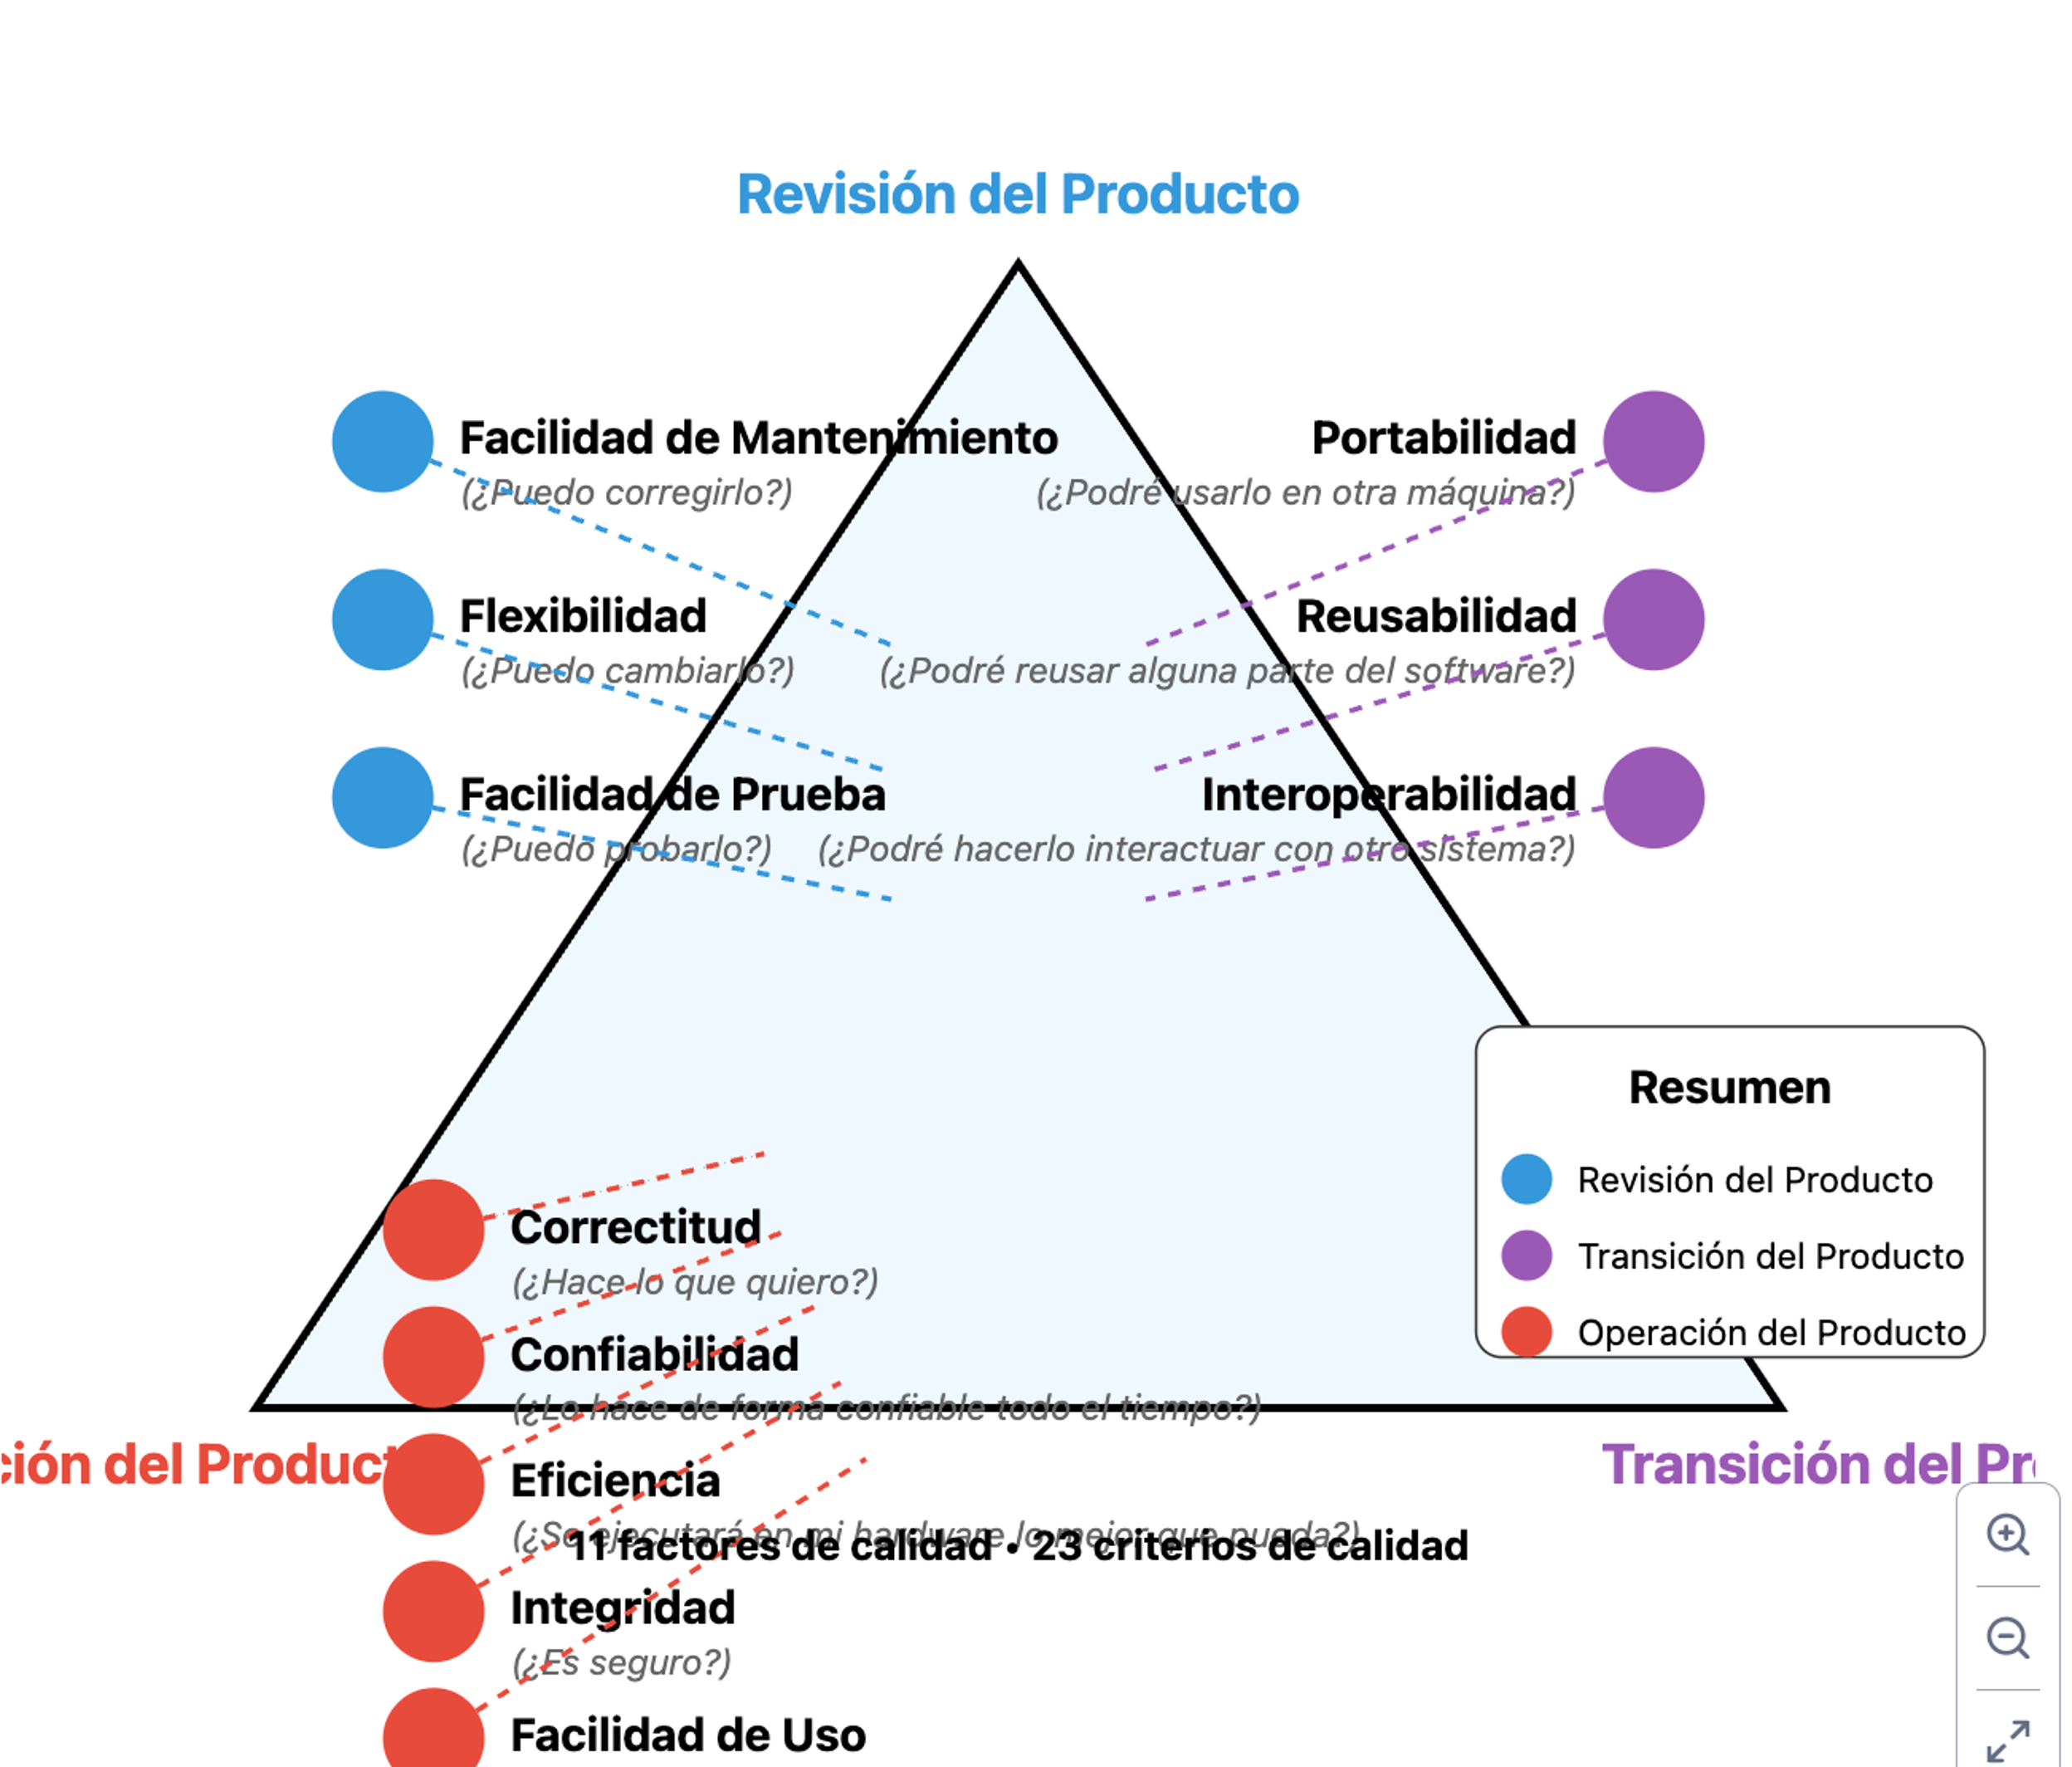
\includegraphics[width=0.8\textwidth]{Pictures/mccall.png}
    \caption{Modelo de Calidad de McCall}
    \label{fig:mccall}
\end{figure}

\begin{itemize}
    \item \textbf{Revisión del Producto}:
    \begin{itemize}
        \item Facilidad de Mantenimiento: ¿Puede corregirse el software fácilmente?
        \item Flexibilidad: ¿Puede cambiarse el software para adaptarse a nuevas necesidades?
        \item Facilidad de Prueba: ¿Puede probarse el software de manera efectiva?
    \end{itemize}
    \item \textbf{Transición del Producto}:
    \begin{itemize}
        \item Portabilidad: ¿Puede usarse el software en diferentes entornos?
        \item Reusabilidad: ¿Pueden reutilizarse partes del software en otros proyectos?
        \item Interoperabilidad: ¿Puede interactuar el software con otros sistemas?
    \end{itemize}
    \item \textbf{Operación del Producto}:
    \begin{itemize}
        \item Correctitud: ¿Hace el software lo que se espera?
        \item Confiabilidad: ¿Funciona el software de manera confiable?
        \item Eficiencia: ¿Utiliza el software los recursos de manera óptima?
        \item Integridad: ¿Es seguro el software?
        \item Facilidad de Uso: ¿Es fácil de usar el software?
    \end{itemize}
\end{itemize}

PD: se recomienda revisar la ISO25000 para un listado más exhaustivo de atributos de calidad.

\section{Conceptos de Diseño y Drivers Arquitectónicos}

Esta sección describe los conceptos de diseño y cómo se relacionan con los impulsores arquitectónicos, separando el diseño de la arquitectura de su evaluación.

\begin{itemize}
\item \textbf{Propósito del Diseño}: Definir el objetivo principal del diseño arquitectónico.
\item \textbf{Funcionalidad Primaria}: Describir las funciones esenciales que el sistema debe cumplir.
\item \textbf{Atributos de Calidad}: Detallar los atributos de calidad que guían las decisiones de diseño, como desempeño, seguridad, y usabilidad.
\item \textbf{Restricciones}: Enumerar las limitaciones que afectan el diseño, como restricciones tecnológicas o de presupuesto.
\item \textbf{Preocupaciones Arquitectónicas}: Identificar las preocupaciones clave que deben abordarse en el diseño.
\item \textbf{Drivers Arquitectónicos}: Especificar los impulsores arquitectónicos que influyen en las decisiones de diseño, como requisitos de negocio, necesidades de los usuarios y condiciones del entorno.
\end{itemize}





\subsection{El Proceso de Diseño Arquitectónico}

El diseño arquitectónico se lleva a cabo en una serie de rondas a lo largo del desarrollo de un proyecto de software. Cada ronda puede ocurrir dentro de un incremento del proyecto, como un sprint. Dentro de estas rondas, se realizan varias iteraciones de diseño. A continuación, se detallan los pasos del proceso de diseño arquitectónico con consejos, explicaciones y ejemplos específicos sobre cómo ejecutarlos:

\begin{enumerate}
    \item \textbf{Revisar las entradas del proceso de diseño:} 
    \begin{itemize}
        \item \textit{Descripción:} Identificar y analizar toda la información relevante que influirá en el diseño, como requisitos del cliente, restricciones tecnológicas y normativas.
        \item \textit{Consejo:} Asegúrate de tener una comprensión clara de los requisitos y limitaciones antes de proceder.
        \item \textit{Ejemplo:} Revisar los requisitos funcionales y no funcionales de una aplicación de comercio electrónico, como la necesidad de manejar 10,000 transacciones por día y cumplir con las normativas de protección de datos.
    \end{itemize}
    
    \item \textbf{Establecer el objetivo de la iteración seleccionando los impulsores:}
    \begin{itemize}
        \item \textit{Descripción:} Definir qué aspectos del sistema se mejorarán o desarrollarán en esta iteración, basándose en los impulsores arquitectónicos.
        \item \textit{Consejo:} Prioriza los impulsores que tengan el mayor impacto en los objetivos del proyecto.
        \item \textit{Ejemplo:} Seleccionar la mejora de la experiencia del usuario en el proceso de pago como objetivo principal de la iteración.
    \end{itemize}
    
    \item \textbf{Elegir uno o más elementos del sistema para refinar:}
    \begin{itemize}
        \item \textit{Descripción:} Seleccionar componentes específicos del sistema que requieren mejoras o ajustes.
        \item \textit{Consejo:} Considera la interdependencia entre componentes para evitar efectos negativos en el sistema.
        \item \textit{Ejemplo:} Decidir refinar el módulo de pago para reducir el tiempo de procesamiento y mejorar la seguridad.
    \end{itemize}
    
    \item \textbf{Seleccionar conceptos de diseño que satisfagan los impulsores seleccionados:}
    \begin{itemize}
        \item \textit{Descripción:} Identificar y aplicar principios de diseño que aborden los impulsores seleccionados.
        \item \textit{Consejo:} Evalúa diferentes enfoques de diseño y elige el que mejor se alinee con los objetivos del proyecto.
        \item \textit{Ejemplo:} Aplicar un diseño de microservicios para el módulo de pago que permita escalabilidad y actualizaciones independientes.
    \end{itemize}
    
    \item \textbf{Instanciar elementos arquitectónicos y definir interfaces:}
    \begin{itemize}
        \item \textit{Descripción:} Crear instancias de los elementos arquitectónicos y definir cómo interactuarán entre sí.
        \item \textit{Consejo:} Asegúrate de que las interfaces sean claras y bien documentadas para facilitar la integración.
        \item \textit{Ejemplo:} Definir interfaces API RESTful para el módulo de pago que permitan la comunicación con el sistema de inventario y el sistema de usuarios.
    \end{itemize}
    
    \item \textbf{Documentar vistas y decisiones de diseño:}
    \begin{itemize}
        \item \textit{Descripción:} Registrar las decisiones de diseño y las vistas arquitectónicas para referencia futura.
        \item \textit{Consejo:} Utiliza diagramas y descripciones detalladas para comunicar efectivamente el diseño a todos los interesados.
        \item \textit{Ejemplo:} Crear diagramas de componentes y secuencia que muestren cómo el módulo de pago interactúa con otros módulos del sistema de comercio electrónico.
    \end{itemize}
    
    \item \textbf{Realizar análisis del diseño actual:}
    \begin{itemize}
        \item \textit{Descripción:} Evaluar el diseño para identificar áreas de mejora y asegurar que cumple con los requisitos.
        \item \textit{Consejo:} Involucra a diferentes partes interesadas en el análisis para obtener una perspectiva completa.
        \item \textit{Ejemplo:} Realizar una revisión de diseño con el equipo de desarrollo y los stakeholders para asegurar que el módulo de pago cumple con los estándares de seguridad y rendimiento.
    \end{itemize}
\end{enumerate}


\color{blue}
\subsection{Caso de Estudio: Hospital Rural Integrado a la Ficha Clínica Nacional}

Este caso de estudio se centra en un hospital rural con limitaciones tecnológicas que se ha integrado recientemente a la ficha clínica nacional administrada por el MINSAL. El hospital cuenta con un sistema de información de agenda electrónica, notificaciones por SMS y WhatsApp, y un subsistema para la gestión de inventario de insumos médicos, agenda de pabellones, y un sistema de recursos humanos y finanzas.

\begin{itemize}
    \item \textbf{Propósito del Diseño}: Visualizar la arquitectura existente del hospital para comprender mejor los sistemas integrados y su interacción.
    \item \textbf{Funcionalidad Primaria}: Identificar y documentar las funciones esenciales de los sistemas actuales, como la gestión de citas, notificaciones, y administración de inventario y recursos.
    \item \textbf{Atributos de Calidad}: Evaluar la interoperabilidad, seguridad, y eficiencia de los sistemas existentes.
    \item \textbf{Restricciones}: Considerar las limitaciones tecnológicas del hospital y la falta de acceso al código fuente para realizar ingeniería inversa.
    \item \textbf{Preocupaciones Arquitectónicas}: Asegurar que la visualización de la arquitectura refleje con precisión la integración con la ficha clínica nacional y otros subsistemas.
    \item \textbf{Drivers Arquitectónicos}: Mejorar la comprensión de la arquitectura para facilitar futuras mejoras y asegurar el cumplimiento con las normativas del MINSAL.
\end{itemize}

%%%%%%%%%%%%%%
\subsubsection{Revisar las Entradas del Proceso de Diseño}

\begin{itemize}
    \item \textbf{Escenario 1: Gestión de Citas Médicas}
    \begin{itemize}
        \item \textbf{Requerimiento Funcional:} Permitir la programación y modificación de citas médicas.
        \item \textbf{Atributo de Calidad:} Disponibilidad
        \item \textbf{Métrica y Valores Esperados:} Sistema disponible 24/7, tiempo de inactividad menor a 1 hora por mes.
    \end{itemize}
    \item \textbf{Escenario 2: Notificaciones a Pacientes}
    \begin{itemize}
        \item \textbf{Requerimiento Funcional:} Enviar notificaciones por SMS y WhatsApp.
        \item \textbf{Atributo de Calidad:} Usabilidad
        \item \textbf{Métrica y Valores Esperados:} Configuración intuitiva, comprensión del 95% de los usuarios.
    \end{itemize}
    \item \textbf{Escenario 3: Gestión de Inventario de Insumos Médicos}
    \begin{itemize}
        \item \textbf{Requerimiento Funcional:} Controlar el stock y generar alertas de reposición.
        \item \textbf{Atributo de Calidad:} Fiabilidad
        \item \textbf{Métrica y Valores Esperados:} Actualización en tiempo real, precisión del 99%.
    \end{itemize}
    \item \textbf{Escenario 4: Acceso a la Ficha Clínica Nacional}
    \begin{itemize}
        \item \textbf{Requerimiento Funcional:} Integración con la ficha clínica nacional.
        \item \textbf{Atributo de Calidad:} Interoperabilidad
        \item \textbf{Métrica y Valores Esperados:} Integración sin errores, tiempo de respuesta menor a 2 segundos.
    \end{itemize}
    \item \textbf{Escenario 5: Sistema de Recursos Humanos y Finanzas}
    \begin{itemize}
        \item \textbf{Requerimiento Funcional:} Gestionar la nómina y recursos humanos.
        \item \textbf{Atributo de Calidad:} Mantenibilidad
        \item \textbf{Métrica y Valores Esperados:} Actualizaciones sin interrupciones, tiempo de implementación menor a 1 día.
    \end{itemize}
\end{itemize}
Estas son las funcionalidades que provee el sistema actualmente: 
\begin{itemize}
    \item RF1: El sistema permitirá la programación de citas médicas por parte del personal administrativo.
    \item RF2: El sistema permitirá la modificación de citas médicas ya programadas.
    \item RF3: El sistema permitirá la cancelación de citas médicas.
    \item RF4: El sistema enviará notificaciones por SMS a los pacientes para recordarles sus citas.
    \item RF5: El sistema enviará notificaciones por WhatsApp a los pacientes para recordarles sus citas.
    \item RF6: El sistema enviará notificaciones a los médicos sobre sus citas programadas.
    \item RF7: El sistema proporcionará un panel de control para que el personal administrativo gestione todas las citas.
    \item RF8: El sistema controlará el stock de insumos médicos.
    \item RF9: El sistema permitirá el acceso a la ficha clínica nacional para los médicos autorizados.
    \item RF10: El sistema gestionará la nómina del personal del hospital.
    \item RF11: El sistema permitirá la gestión de datos de los empleados, como horarios y permisos.
    \item RF12: El sistema debe integrarse con otros sistemas de salud para el intercambio de datos.
    \item RF13: Los datos deben encriptarse durante su tráfico y almacenamiento.
    \item RF14: El sistema debe requerir autenticación de usuario para acceder a sus funcionalidades.
    \item RF15: El sistema debe mantener logs detallados para auditoría y seguimiento de actividades.
    \item RF16: El sistema debe estar disponible 24/7 con un tiempo de inactividad menor a 1 hora por mes.
    \item RF17: La interfaz debe ser fácil de usar para el personal médico y administrativo.
    \item RF18: El sistema debe optimizar el uso de recursos para asegurar un rendimiento óptimo.
    \item RF19: El sistema debe generar alertas automáticas para la reposición de insumos médicos.
    \item RF20: El sistema debe permitir la adición de nuevos ítems y funcionalidades sin afectar el rendimiento.
    \item RF21: El sistema debe permitir la trazabilidad de todas las acciones realizadas por los usuarios.
\end{itemize}


Es crucial considerar las restricciones tecnológicas y normativas que pueden influir en el diseño del sistema. Entre estas restricciones se incluyen:

\begin{itemize}
    \item \textbf{Ley de Protección de Datos Personales de Chile:} Cumplimiento con la Ley N° 19.628 para proteger la información sensible de los pacientes.
    \item \textbf{Interoperabilidad de la Ficha Clínica Electrónica:} Asegurar que el sistema cumpla con las normativas de interoperabilidad establecidas por el Ministerio de Salud de Chile.
    \item \textbf{Limitaciones Tecnológicas:} En un hospital rural, existe una restricción tecnológica como la conectividad limitada a internet, lo que afectaría la capacidad de sincronización de datos en tiempo real.
\end{itemize}







%%%%%%%%
\subsubsection{Establecer el Objetivo de la Iteración Seleccionando los Impulsores}

\textbf{Descripción:} Definir qué aspectos del sistema del hospital rural se mejorarán o desarrollarán en esta iteración, basándose en los impulsores arquitectónicos identificados.

\textbf{Consejo:} Prioriza los impulsores que tengan el mayor impacto en los objetivos del proyecto, especialmente aquellos que mejoren la mantenibilidad y la visibilidad del sistema.

\textbf{Ejemplo:}
\begin{itemize}
    \item \textbf{Mejora de la Mantenibilidad:}
    \begin{itemize}
        \item \textit{Impulsor:} Reducir la complejidad del código y mejorar la documentación.
        \item \textit{Objetivo:} Facilitar el mantenimiento y la actualización del sistema, permitiendo cambios más rápidos y menos propensos a errores.
    \end{itemize}
    \item \textbf{Visibilización del Sistema:}
    \begin{itemize}
        \item \textit{Impulsor:} Crear una representación clara de la arquitectura actual.
        \item \textit{Objetivo:} Documentar la arquitectura, identificando componentes clave y sus interacciones.
    \end{itemize}
    \item \textbf{Mejora de la Interoperabilidad:}
    \begin{itemize}
        \item \textit{Impulsor:} Asegurar que el sistema se integre eficazmente con otros sistemas de salud.
        \item \textit{Objetivo:} Mejorar la capacidad del sistema para comunicarse con la ficha clínica nacional y otros sistemas hospitalarios.
    \end{itemize}
\end{itemize}


\subsubsection{Elegir uno o más Elementos del Sistema para Refinar}
% Aquí se detallarán los pasos para elegir elementos del sistema a refinar.

% \item \textbf{Elegir uno o más elementos del sistema para refinar:}
% \begin{itemize}
%     \item \textit{Descripción:} Seleccionar componentes específicos del sistema que requieren mejoras o ajustes.
%     \item \textit{Consejo:} Considera la interdependencia entre componentes para evitar efectos negativos en el sistema.
%     \item \textit{Ejemplo:} Decidir refinar el módulo de pago para reducir el tiempo de procesamiento y mejorar la seguridad.
% \end{itemize}
Refinaremos interoperabilidad y disponibilidad con sistemas externos. 

El siguiente diagrama muestra el despliegue del sistema dada la instalación actual, no incluyendo los subsistemas o componentes existentes para recursos humanos, finanzas, entre otros.

\begin{figure}[h]
\centering
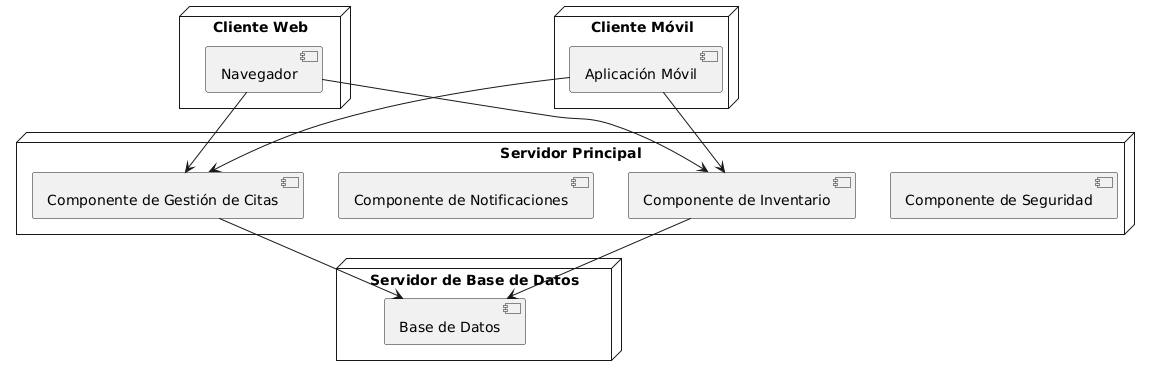
\includegraphics[width=\textwidth]{diagramadespliegue.png}
\caption{Diagrama de Despliegue del Sistema Completo}
\label{fig:complete_deployment_diagram}
\end{figure}


\begin{table}[h]
    \centering
    \begin{tabular}{|l|p{10cm}|}
    \hline
    \textbf{Escenario} & \textbf{Requerimientos Funcionales} \\ \hline
    \textbf{Gestión de Citas Médicas} & 
    \begin{itemize}
        \item RF1: El sistema permitirá la programación de citas médicas por parte del personal administrativo.
        \item RF2: El sistema permitirá la modificación de citas médicas ya programadas.
        \item RF3: El sistema permitirá la cancelación de citas médicas.
    \end{itemize} \\ \hline
    \textbf{Notificaciones a Pacientes*} & 
    \begin{itemize}
        \item RF4: El sistema enviará notificaciones por SMS a los pacientes para recordarles sus citas.
        \item RF5: El sistema enviará notificaciones por WhatsApp a los pacientes para recordarles sus citas.
        \item RF6: El sistema enviará notificaciones a los médicos sobre sus citas programadas.
    \end{itemize} \\ \hline
    \textbf{Gestión de Inventario de Insumos Médicos} & 
    \begin{itemize}
        \item RF8: El sistema controlará el stock de insumos médicos.
        \item RF19: El sistema debe generar alertas automáticas para la reposición de insumos médicos.
    \end{itemize} \\ \hline
    \textbf{Acceso a la Ficha Clínica Nacional} & 
    \begin{itemize}
        \item RF9: El sistema permitirá el acceso a la ficha clínica nacional para los médicos autorizados.
        \item RF12: El sistema debe integrarse con otros sistemas de salud para el intercambio de datos.
    \end{itemize} \\ \hline
    \textbf{Sistema de Recursos Humanos y Finanzas} & 
    \begin{itemize}
        \item RF10: El sistema gestionará la nómina del personal del hospital.
        \item RF11: El sistema permitirá la gestión de datos de los empleados, como horarios y permisos.
    \end{itemize} \\ \hline
    \end{tabular}
    \caption{Cruce de Escenarios con Requerimientos Funcionales}
    \label{tab:escenarios_requerimientos}
    \end{table}

Dijimos \textbf{Mejora de la Mantenibilidad}, y \textbf{Mejora de la Interoperabilidad} y el escenario  \textbf{Acceso a la Ficha Clínica Nacional} - RF9: El sistema permitirá el acceso a la ficha clínica nacional para los médicos autorizados. Para eso lo primero es crear un escenario detallado que nos servirá para una prueba de aceptación: 

\textbf{Escenario Detallado: Acceso a la Ficha Clínica Nacional}

\textbf{Contexto:} En un hospital rural, un médico está atendiendo a un paciente que ha sido derivado desde otro centro de salud. Durante la consulta, el médico necesita acceder a la ficha clínica nacional para revisar el historial médico del paciente, incluyendo diagnósticos previos, tratamientos y alergias conocidas. Este acceso es crucial para tomar decisiones informadas sobre el tratamiento actual del paciente.

\textbf{Requerimiento Funcional:} RF9: El sistema permitirá el acceso a la ficha clínica nacional para los médicos autorizados.

\textbf{Atributos de Calidad:}
\begin{itemize}
    \item \textbf{Interoperabilidad:} El sistema debe integrarse sin problemas con la ficha clínica nacional.
    \item \textbf{Seguridad:} El acceso debe ser seguro, garantizando la protección de los datos del paciente.
    \item \textbf{Disponibilidad:} El sistema debe estar disponible 24/7 para asegurar que los médicos puedan acceder a la información cuando sea necesario.
\end{itemize}

\textbf{Métrica y Valores Esperados:}
\begin{itemize}
    \item Tiempo de respuesta para acceder a la ficha clínica: menos de 2 segundos.
    \item Cumplimiento con las normativas de protección de datos personales.
\end{itemize}


\begin{figure}[h]
    \centering
    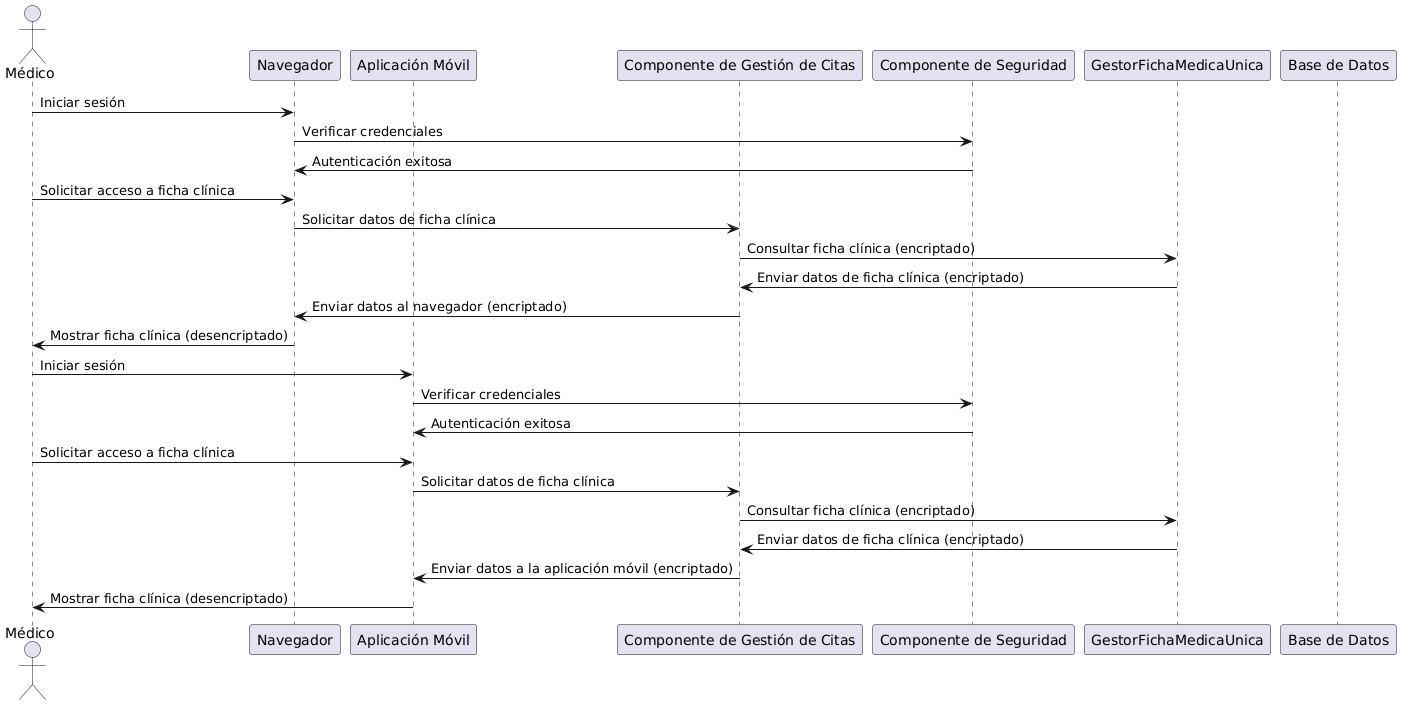
\includegraphics[width=\textwidth]{diagramasecuencia.png}
    \caption{Diagrama de Secuencia para el Escenario de Acceso a la Ficha Clínica Nacional}
    \label{fig:diagrama_secuencia}
\end{figure}
Ver más detalles en las slides de cómo ir verificando que si se cumple o no o si se debe seguir iterando. 

\subsubsection{Seleccionar Conceptos de Diseño que Satisfagan los Impulsores Seleccionados}
% Aquí se detallarán los pasos para seleccionar conceptos de diseño.

% \item \textbf{Seleccionar conceptos de diseño que satisfagan los impulsores seleccionados:}
% \begin{itemize}
%     \item \textit{Descripción:} Identificar y aplicar principios de diseño que aborden los impulsores seleccionados.
%     \item \textit{Consejo:} Evalúa diferentes enfoques de diseño y elige el que mejor se alinee con los objetivos del proyecto.
%     \item \textit{Ejemplo:} Aplicar un diseño de microservicios para el módulo de pago que permita escalabilidad y actualizaciones independientes.
% \end{itemize}

\subsubsection{Seleccionar Conceptos de Diseño que Satisfagan los Impulsores Seleccionados}

Dado los drivers arquitectónicos identificados, que incluyen la mejora de la mantenibilidad, la mejora de la interoperabilidad y el acceso a la ficha clínica nacional, hemos seleccionado un concepto de diseño que se enfoca en la redundancia, alta disponibilidad e interoperabilidad, adaptado a las limitaciones de un hospital rural con sistemas antiguos.

\textbf{Drivers Arquitectónicos:}
\begin{itemize}
    \item \textbf{Mejora de la Mantenibilidad:} Asegurar que el sistema pueda ser corregido y actualizado fácilmente, incluso con infraestructura antigua.
    \item \textbf{Mejora de la Interoperabilidad:} Garantizar que el sistema pueda interactuar sin problemas con otros sistemas, como la ficha clínica nacional proporcionada por el gobierno.
    \item \textbf{Acceso a la Ficha Clínica Nacional:} Permitir a los médicos autorizados acceder a la ficha clínica nacional de manera segura y eficiente.
\end{itemize}

Para abordar estos drivers, el gobierno ha adoptado un diseño que maximiza el uso de la infraestructura existente, integrando servicios gubernamentales para la ficha médica. Se ha implementado redundancia y alta disponibilidad mediante configuraciones de respaldo y sistemas de failover, asegurando que el sistema esté siempre disponible y pueda manejar fallos sin interrumpir el servicio.

\textbf{Nuevos Diagramas:}

\begin{figure}[h]
    \centering
    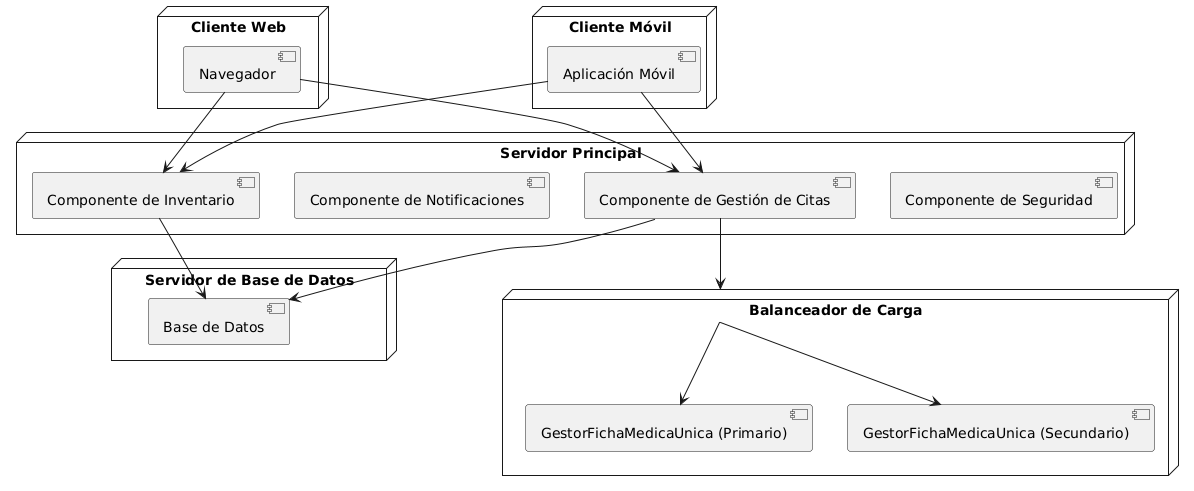
\includegraphics[width=\textwidth]{diagramadespliegue2.png}
    \caption{Diagrama de Despliegue con Alta Disponibilidad e Interoperabilidad}
    \label{fig:diagrama_despliegue2}
\end{figure}

El \textbf{Diagrama de Despliegue} muestra cómo los componentes del sistema están distribuidos en la infraestructura existente del hospital, utilizando servidores de respaldo para asegurar alta disponibilidad. Cada componente crítico tiene un sistema de failover, lo que permite que el sistema continúe funcionando incluso si uno de los servidores falla. Además, se utilizan configuraciones de red para asegurar que las solicitudes se redirijan adecuadamente en caso de fallos.

\begin{figure}[h]
    \centering
    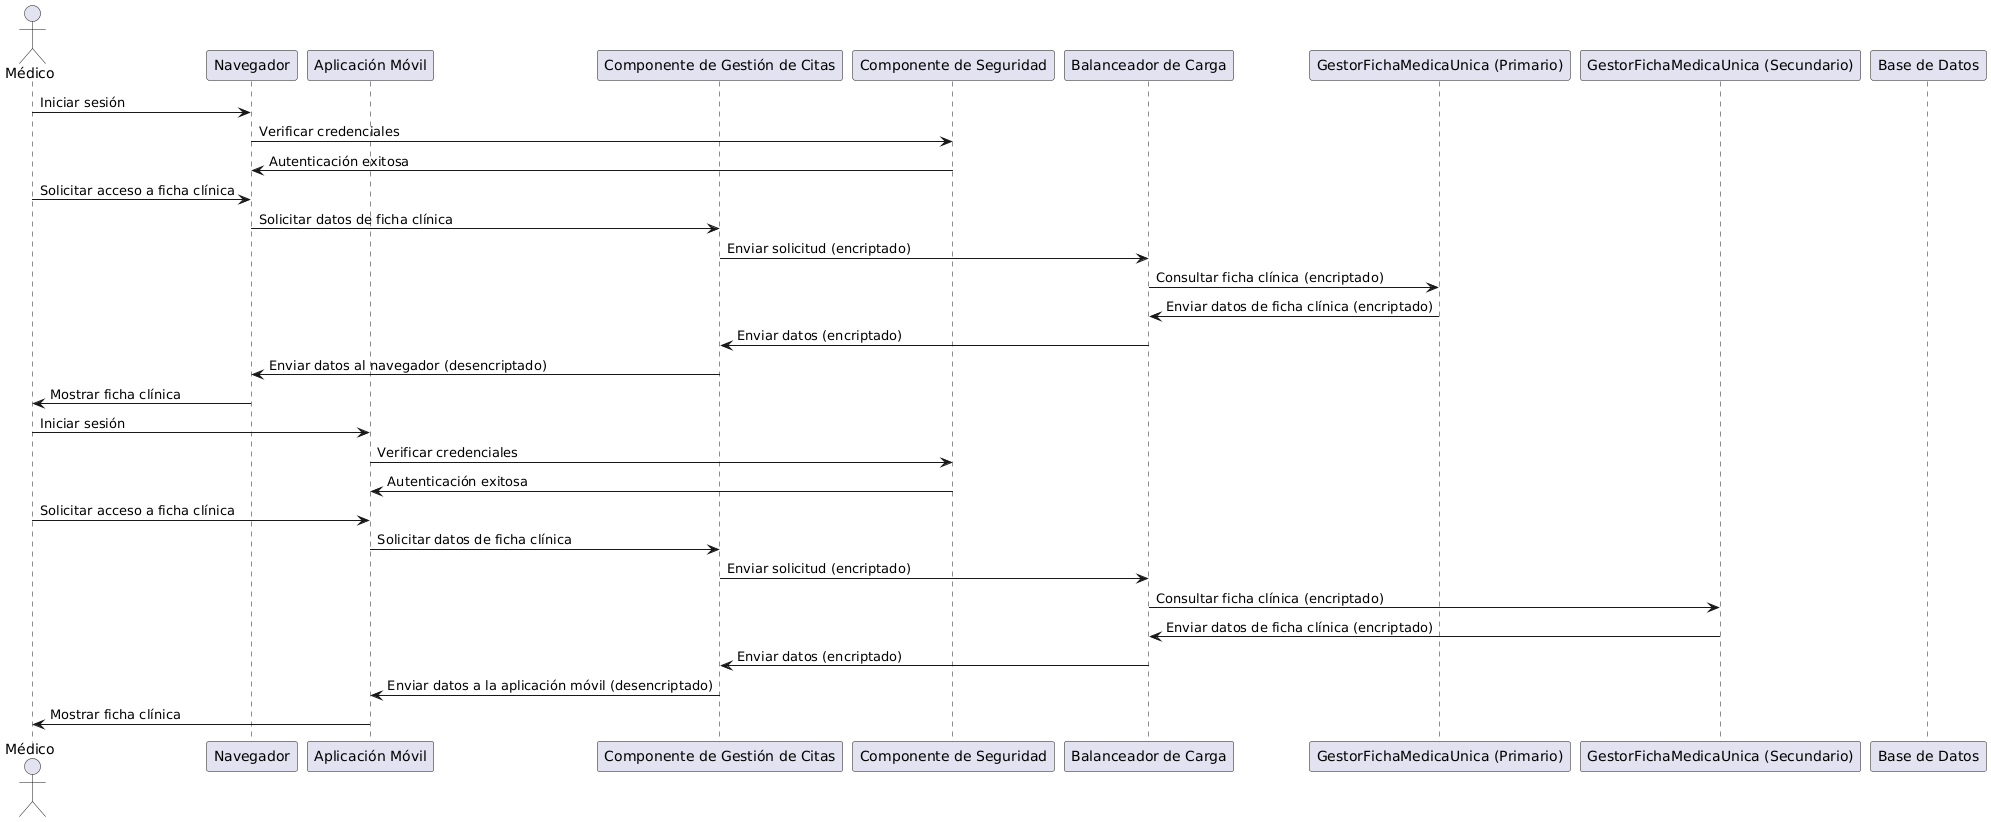
\includegraphics[width=\textwidth]{diagramasecuencia2.png}
    \caption{Diagrama de Secuencia para el Escenario de Acceso a la Ficha Clínica Nacional con Alta Disponibilidad}
    \label{fig:diagrama_secuencia2}
\end{figure}

El \textbf{Diagrama de Secuencia} actualizado muestra el flujo de interacción entre los componentes del sistema durante el acceso a la ficha clínica nacional. Este diagrama destaca cómo se maneja la redundancia y la alta disponibilidad en el proceso. Si un componente falla, el sistema redirige automáticamente la solicitud a un sistema de respaldo, asegurando que el acceso a la ficha clínica no se vea interrumpido.

Estos nuevos diseños no solo cubren los drivers arquitectónicos identificados, sino que también mejoran la resiliencia y la eficiencia del sistema, asegurando que los médicos puedan acceder a la información crítica del paciente en todo momento, incluso con las limitaciones de un entorno rural.


Para asegurar la integridad y confidencialidad de los datos en sistemas de información, se han considerado varias alternativas tecnológicas. A continuación, se presentan algunas de las opciones más relevantes:

\textbf{1. Uso de X-Road de Estonia:}
X-Road es una solución de intercambio de datos segura y escalable utilizada en Estonia. Permite la comunicación segura entre diferentes sistemas de información, garantizando la integridad y confidencialidad de los datos. Implementar X-Road podría proporcionar una capa adicional de seguridad y asegurar que los datos intercambiados entre diferentes entidades sean protegidos contra accesos no autorizados.

\textbf{2. Contratos Inteligentes con Neuroledger:}
Neuroledger es una plataforma que utiliza contratos inteligentes para asegurar la integridad de los datos. Los contratos inteligentes pueden verificar automáticamente la autenticidad de los datos y asegurar que no hayan sido alterados. Esta solución podría ser implementada para garantizar que los datos sean confiables y estén protegidos contra manipulaciones.

\textbf{3. Hashing de Datos:}
Una solución más sencilla podría ser el uso de hashes para verificar la integridad de los datos. Cada vez que se intercambian datos entre entidades, se podría generar un hash que se verifique en ambos extremos. Aunque esta solución es más casera, puede ser efectiva para asegurar que los datos no hayan sido alterados durante la transmisión.

\textbf{4. Encriptación de Datos:}
Para asegurar la confidencialidad de los datos, es esencial implementar encriptación. Los datos sensibles deben ser encriptados tanto en tránsito como en reposo. Esto asegurará que, incluso si los datos son interceptados, no puedan ser leídos por personas no autorizadas.

\textbf{5. Autenticación y Autorización:}
No se ha discutido en detalle cómo se manejará la autenticación y autorización en los sistemas de información. Es crucial explorar opciones como OAuth 2.0 y OpenID Connect para asegurar que solo usuarios autorizados puedan acceder a los datos. OAuth 2.0 proporciona un marco para la autorización segura, mientras que OpenID Connect añade una capa de autenticación, permitiendo verificar la identidad de los usuarios.

\textbf{Tarea para los Alumnos:}
Se recomienda a los alumnos investigar más a fondo estas alternativas de seguridad como una tarea que apoya la nota de participación y compartirla en el foro. Deberán buscar artículos en Medium  para evaluar las ventajas y desventajas de cada opción y proponer una solución que mejor se adapte a las necesidades de los sistemas de información y las limitaciones del entorno en el que se implementen.







\subsubsection{Instanciar Elementos Arquitectónicos y Definir Interfaces}
% Aquí se detallarán los pasos para instanciar elementos arquitectónicos.

% \item \textbf{Instanciar elementos arquitectónicos y definir interfaces:}
% \begin{itemize}
%     \item \textit{Descripción:} Crear instancias de los elementos arquitectónicos y definir cómo interactuarán entre sí.
%     \item \textit{Consejo:} Asegúrate de que las interfaces sean claras y bien documentadas para facilitar la integración.
%     \item \textit{Ejemplo:} Definir interfaces API RESTful para el módulo de pago que permitan la comunicación con el sistema de inventario y el sistema de usuarios.
% \end{itemize}

\textbf{Interfaces Propuestas:}

\begin{itemize}
    \item \textbf{Interface de Gestión de Citas:}
    \begin{itemize}
        \item \textbf{Método:} \texttt{updateAppointment}
        \item \textbf{Parámetros:} Identificador de cita, nueva fecha y hora, detalles del paciente.
        \item \textbf{Retorno:} \texttt{True} si la actualización es exitosa.
        \item \textbf{Excepciones:} \texttt{AppointmentUpdateException} si la actualización falla.
    \end{itemize}
    \item \textbf{Interface de Notificaciones:}
    \begin{itemize}
        \item \textbf{Método:} \texttt{sendNotification}
        \item \textbf{Parámetros:} Identificador del paciente, tipo de notificación (SMS, WhatsApp), mensaje.
        \item \textbf{Retorno:} \texttt{True} si la notificación se envía correctamente.
        \item \textbf{Excepciones:} \texttt{NotificationException} si el envío falla.
    \end{itemize}
    \item \textbf{Interface de Inventario:}
    \begin{itemize}
        \item \textbf{Método:} \texttt{updateStock}
        \item \textbf{Parámetros:} Identificador de insumo, cantidad, fecha de actualización.
        \item \textbf{Retorno:} \texttt{True} si la actualización es exitosa.
        \item \textbf{Excepciones:} \texttt{StockUpdateException} si la actualización falla.
    \end{itemize}
\end{itemize}









\subsubsection{Documentar Vistas y Decisiones de Diseño}
% Aquí se detallarán los pasos para documentar vistas y decisiones de diseño.
% \item \textbf{Documentar vistas y decisiones de diseño:}
% \begin{itemize}
%     \item \textit{Descripción:} Registrar las decisiones de diseño y las vistas arquitectónicas para referencia futura.
%     \item \textit{Consejo:} Utiliza diagramas y descripciones detalladas para comunicar efectivamente el diseño a todos los interesados.
%     \item \textit{Ejemplo:} Crear diagramas de componentes y secuencia que muestren cómo el módulo de pago interactúa con otros módulos del sistema de comercio electrónico.
% \end{itemize}


Las vistas de la arquitectura se dividen en varias categorías, cada una enfocada en un aspecto particular del sistema:

\textbf{Vista de Componentes y Conectores:}
\begin{itemize}
    \item \textbf{Propósito:} Mostrar los componentes principales del sistema y cómo interactúan.
    \item \textbf{Elementos:} componentes, conectores, protocolos de comunicación.
    \item \textbf{Beneficios:} Facilita el análisis de interacción y comunicación entre componentes.
\end{itemize}

\textbf{Vista de Módulos:}
\begin{itemize}
    \item \textbf{Propósito:} Describir la organización del software en módulos y sus relaciones.
    \item \textbf{Elementos:} Módulos, submódulos, dependencias.
    \item \textbf{Beneficios:} Ayuda en la planificación del desarrollo y la asignación de tareas.
\end{itemize}

\textbf{Vista de Despliegue:}
\begin{itemize}
    \item \textbf{Propósito:} Representar cómo el sistema se distribuye en la infraestructura física.
    \item \textbf{Elementos:} Servidores, redes, dispositivos.
    \item \textbf{Beneficios:} Permite evaluar la disponibilidad y redundancia del sistema.
\end{itemize}

\textbf{Vista de Ejecución:}
\begin{itemize}
    \item \textbf{Propósito:} Mostrar cómo se comporta el sistema durante la ejecución.
    \item \textbf{Elementos:} Procesos, hilos, interacciones en tiempo real.
    \item \textbf{Beneficios:} Ayuda a identificar cuellos de botella y optimizar el rendimiento.
\end{itemize}

\textbf{Importancia}

Estas vistas no solo proporcionan un mapa para la construcción del código, sino que también facilitan el análisis de impacto, la planificación del desarrollo incremental y la trazabilidad de requisitos. Al documentar las vistas arquitectónicas, se asegura que todos los interesados tengan una comprensión clara del sistema, lo que es crucial para la colaboración efectiva y la toma de decisiones informadas.

Este resumen proporciona una visión general de las vistas arquitectónicas y su importancia en el diseño de software. Si necesitas más detalles o ejemplos específicos, házmelo saber.


Las vistas arquitectónicas son esenciales para proporcionar una representación estructurada del sistema. Permiten a los desarrolladores y arquitectos comprender cómo los componentes interactúan entre sí y cómo se integran en el entorno operativo. Estas vistas son cruciales para:
\begin{itemize}
    \item \textbf{Razonar sobre Atributos de Calidad:} Como rendimiento, confiabilidad y disponibilidad.
    \item \textbf{Predicción del Comportamiento del Sistema:} Bajo diferentes condiciones.
    \item \textbf{Análisis de Impacto:} Facilitan la evaluación de cómo los cambios en un componente pueden afectar al sistema en su conjunto.
    \item \textbf{Colaboración Efectiva:} Aseguran que todos los interesados tengan una comprensión clara del sistema, lo que es crucial para la toma de decisiones informadas.
\end{itemize}




Esto lo veremos más adelante usando otros enfoques. 

\subsubsection{Realizar Análisis del Diseño Actual}
% Aquí se detallarán los pasos para realizar el análisis del diseño actual.
% \item \textbf{Realizar análisis del diseño actual:}
% \begin{itemize}
%     \item \textit{Descripción:} Evaluar el diseño para identificar áreas de mejora y asegurar que cumple con los requisitos.
%     \item \textit{Consejo:} Involucra a diferentes partes interesadas en el análisis para obtener una perspectiva completa.
%     \item \textit{Ejemplo:} Realizar una revisión de diseño con el equipo de desarrollo y los stakeholders para asegurar que el módulo de pago cumple con los estándares de seguridad y rendimiento.
% \end{itemize}
% \end{enumerate}
Esto lo veremos más adelante usando otros enfoques. 
\color{black}























\section{El Modelo C4 para Visualizar la Arquitectura de Software}

El modelo C4 es una forma de ayudar a los equipos de desarrollo de software a describir y comunicar la arquitectura de software, tanto durante las sesiones de diseño iniciales como al documentar retrospectivamente una base de código existente. Es una manera de crear "mapas de tu código" en varios niveles de detalle, de la misma manera que usarías algo como Google Maps para acercarte y alejarte de un área de interés.

\subsection{Historia y Evolución del Modelo C4}
El modelo C4 fue creado por Simon Brown como una respuesta a la falta de claridad y consistencia en los diagramas de arquitectura de software. A menudo, los diagramas de software son una mezcla confusa de cajas y líneas sin una notación consistente, lo que dificulta la comunicación efectiva. El modelo C4 busca mejorar la madurez de los diagramas de arquitectura de software al proporcionar un conjunto de abstracciones jerárquicas y diagramas que son independientes de la notación y las herramientas.

\subsection{Abstracciones del Modelo C4}
El modelo C4 se basa en un conjunto de abstracciones jerárquicas que reflejan cómo los arquitectos y desarrolladores de software piensan y construyen software. Estas abstracciones incluyen:

\begin{itemize}
    \item \textbf{Sistema de Software}: El nivel más alto de abstracción que describe algo que entrega valor a sus usuarios.
    \item \textbf{Contenedor}: Representa una aplicación o un almacén de datos que necesita estar en funcionamiento para que el sistema de software funcione.
    \item \textbf{Componente}: Un grupo de funcionalidades relacionadas encapsuladas detrás de una interfaz bien definida.
    \item \textbf{Código}: Elementos de código que implementan los componentes, como clases, interfaces, objetos, funciones, etc.
\end{itemize}

\subsection{Diagramas del Modelo C4}
El modelo C4 utiliza un conjunto de diagramas jerárquicos para visualizar la arquitectura de software:

\begin{itemize}
    \item \textbf{Diagrama de Contexto del Sistema}: Muestra cómo el sistema de software se integra en el mundo que lo rodea.
    \item \textbf{Diagrama de Contenedores}: Detalla las aplicaciones y almacenes de datos dentro del sistema de software.
    \item \textbf{Diagrama de Componentes}: Muestra los componentes dentro de un contenedor individual.
    \item \textbf{Diagrama de Código}: Puede usarse para mostrar cómo se implementa un componente a nivel de código.
\end{itemize}

\subsection{Beneficios y Debilidades del Modelo C4}
El modelo C4 ofrece varios beneficios, como la claridad en la comunicación de la arquitectura de software y la facilidad de aprendizaje y uso debido a su pequeño conjunto de abstracciones y tipos de diagramas. Sin embargo, también tiene debilidades, como la posible falta de detalle en sistemas muy complejos y la necesidad de complementarlo con otros tipos de diagramas para cubrir aspectos dinámicos o de despliegue.

\subsection{Método para Construir la Arquitectura del Hospital con DART usando el Modelo C4}
Este método combina el modelo C4 con los enfoques previamente discutidos, garantizando que el diseño de la arquitectura del sistema DART sea consistente y fácil de entender. A continuación, se presentan los pasos detallados que los estudiantes deben seguir para crear diagramas en PlantUML, bajo la guía del instructor.




\subsubsection{Paso 1: Diagrama de Contexto del Sistema Hospitalario con Exámenes Remotos}

\begin{itemize}
    \item \textbf{Descripción}: Este diagrama proporciona una visión general del sistema hospitalario, destacando la implementación de exámenes remotos a través del sistema DART. Se enfoca en la interacción entre el sistema hospitalario y otros sistemas y usuarios clave, utilizando un enfoque de actor/acción para definir claramente los límites del sistema y sus interacciones actuales y potenciales.
    \item \textbf{Instrucciones}:
    \begin{itemize}
        \item Identificar los actores principales que interactúan con el sistema hospitalario, como el Técnico en Telemedicina, el Sistema IA y el Oftalmólogo. Estos actores representan a las personas o sistemas externos que se comunican con el sistema hospitalario.
        \item Identificar los sistemas externos con los que el sistema hospitalario interactúa, como el Sistema de Información Hospitalaria y el sistema DART. Estos son sistemas que proporcionan o reciben información del sistema hospitalario.
        \item Asegurar que las interacciones estén claramente etiquetadas para facilitar la comprensión del flujo de información y considerar futuras integraciones con otros sistemas de diagnóstico remoto.
    \end{itemize}
    \item \textbf{PlantUML}:
    \begin{verbatim}
    @startuml
    actor "Técnico en Telemedicina" as TT
    actor "Oftalmólogo" as O
    package "Sistema Hospitalario" {
        [Sistema Hospitalario]
    }
    [Sistema Hospitalario] --> TT : Supervisión de Exámenes
    [Sistema Hospitalario] --> O : Validación de Diagnósticos
    [Sistema Hospitalario] --> [Sistema de Información Hospitalaria] : Integración de Datos
    [Sistema Hospitalario] --> [Sistema DART] : Análisis de Imágenes
    @enduml
    \end{verbatim}
\end{itemize}

El diagrama de contexto (Figura \ref{fig:dart_context}) ilustra las interacciones entre los diferentes actores y sistemas. Los elementos se representan utilizando la notación C4, donde las personas se muestran en azul, los sistemas internos en celeste y los sistemas externos en gris.

\begin{figure}[h]
    \centering
    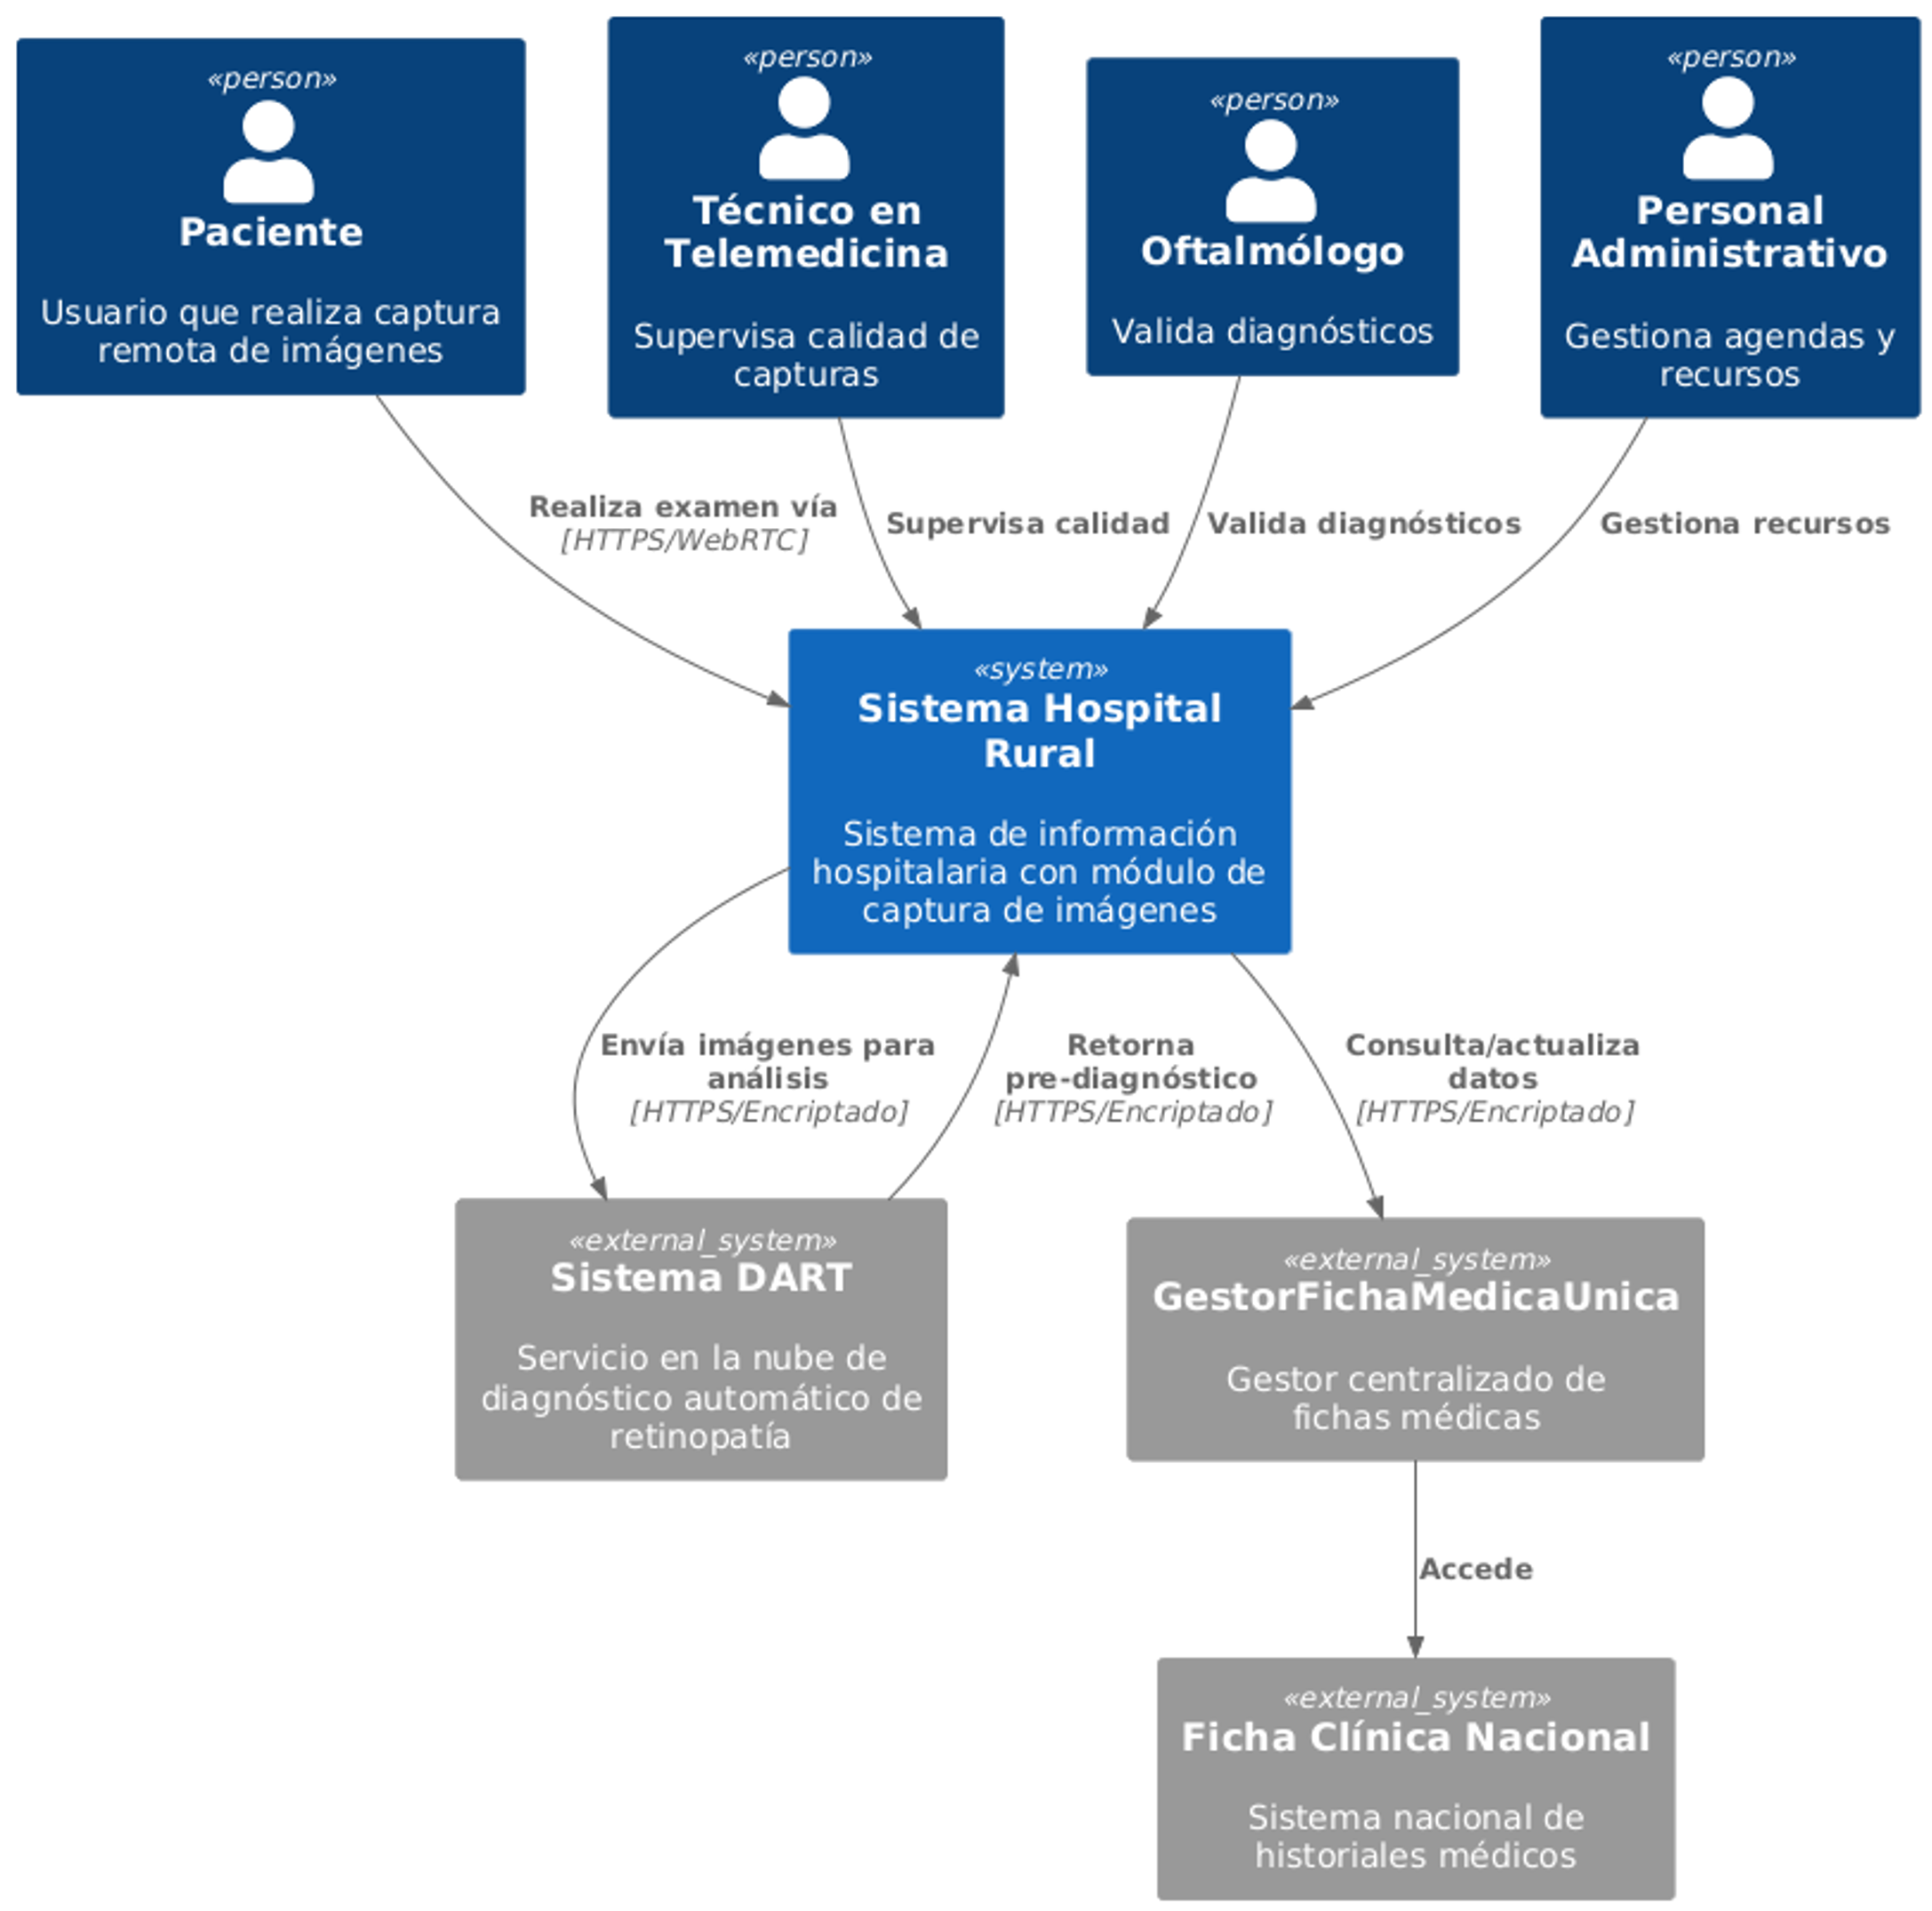
\includegraphics[width=\textwidth]{Pictures/dart_context.png}
    \caption{Diagrama de Contexto del Sistema DART integrado con el Hospital Rural}
    \label{fig:dart_context}
\end{figure}

En esta arquitectura, el Sistema de Información Hospitalaria (HIS) actúa como punto central de interacción para todos los usuarios. El paciente realiza el examen de retinopatía conectándose directamente al HIS a través de su navegador web, utilizando WebRTC para la captura de imágenes. El sistema DART, al igual que la Ficha Clínica Nacional, opera como un servicio en la nube, invisible para el usuario final. En el centro del diagrama se encuentra el Sistema DART, que interactúa con cuatro tipos de usuarios principales: el paciente, que ahora puede realizar capturas remotas de imágenes retinales; el técnico en telemedicina, que supervisa la calidad de estas capturas; el oftalmólogo, que valida los diagnósticos; y el personal administrativo, que gestiona los recursos y agendas del sistema.

La implementación utiliza tecnología WebRTC para la captura de imágenes a través del navegador, lo que elimina la necesidad de software especializado en el computador del paciente. Esta decisión arquitectónica simplifica significativamente el despliegue y la adopción del sistema, requiriendo únicamente:
\begin{itemize}
    \item Un navegador web moderno con soporte para WebRTC
    \item Una cámara web con resolución mínima de 720p
    \item Una conexión a internet estable (mínimo 1Mbps de subida)
\end{itemize}

El flujo de trabajo típico es el siguiente:
\begin{enumerate}
    \item El paciente accede al portal del hospital (HIS) para realizar su examen
    \item El HIS gestiona la captura de imágenes a través del navegador del paciente
    \item Las imágenes capturadas se envían al servicio DART en la nube para su análisis
    \item DART procesa las imágenes y retorna un pre-diagnóstico al HIS
    \item El técnico en telemedicina y/o el oftalmólogo revisan los resultados a través del HIS
    \item Una vez validado el diagnóstico, se actualiza la ficha del paciente a través del GestorFichaMedicaUnica
\end{enumerate}

Esta arquitectura distribuida ofrece varias ventajas:
\begin{itemize}
    \item Centralización de la interacción del usuario en el sistema hospitalario
    \item Procesamiento especializado en la nube mediante el servicio DART
    \item Integración transparente con los sistemas nacionales de salud
    \item Mayor seguridad al manejar datos sensibles a través de canales encriptados
\end{itemize}





\subsubsection{Paso 2: Diagrama de Contenedores}

\begin{itemize}
    \item \textbf{Descripción}: Este diagrama detalla las aplicaciones y almacenes de datos que componen el sistema DART, utilizando la notación del modelo C4. Refleja el enfoque de flujo de trabajo y muestra cómo los diferentes componentes del sistema se comunican entre sí.
    \item \textbf{Instrucciones}:
    \begin{itemize}
        \item Identificar los contenedores principales dentro del sistema hospitalario, como la Aplicación Web y la Base de Datos HIS. Los contenedores son las unidades de software que ejecutan aplicaciones o almacenan datos.
        \item Describir cómo estos contenedores se comunican entre sí y con sistemas externos, especificando las interacciones y el flujo de datos entre ellos.
    \end{itemize}
    \item \textbf{PlantUML}:
    \begin{verbatim}
    @startuml "Sistema Hospitalario"
    !include https://raw.githubusercontent.com/plantuml-stdlib/C4-PlantUML/master/C4_Container.puml

    LAYOUT_WITH_LEGEND()

    title Diagrama de Contenedores para el Sistema Hospitalario

    Person(paciente, "Paciente", "Un paciente que realiza exámenes de retinopatía")
    Person(tecnico, "Técnico en Telemedicina", "Supervisa la calidad de las capturas")
    Person(oftalmologo, "Oftalmólogo", "Valida los diagnósticos")
    Person(admin, "Personal Administrativo", "Gestiona recursos y agendas")

    System_Boundary(sistema_hospitalario, "Sistema Hospitalario") {
        Container(servidor_app, "Servidor de Aplicaciones", "Node.js, npm", "Gestiona las solicitudes de los usuarios y coordina las interacciones con otros sistemas")
        Container(spa, "Aplicación de Página Única", "JavaScript, Angular", "Proporciona toda la funcionalidad de exámenes a los pacientes a través de su navegador web")
        ContainerDb(base_datos_his, "Base de Datos HIS", "MySQL", "Almacena datos de pacientes y exámenes")
        Container(backend_api, "API de Diagnóstico", "Node.js, Docker Container", "Proporciona funcionalidad de diagnóstico a través de API")
    }

    System_Ext(servicio_dart, "Servicio DART", "Análisis de Imágenes en la Nube")
    System_Ext(ficha_clinica_nacional, "Ficha Clínica Nacional", "Sistema Externo")
    System_Ext(gestor_ficha_medica_unica, "Gestor Ficha Médica Única", "Sistema Externo")
    System_Ext(email_system, "Sistema de Correo Electrónico", "Envía notificaciones con informes adjuntos")
    System_Ext(firma_digital, "Servicio de Firma Digital", "Firma digital externa para documentos")

    Rel(paciente, spa, "Usa", "HTTPS")
    Rel(tecnico, spa, "Supervisa calidad de capturas", "HTTPS")
    Rel(oftalmologo, spa, "Valida diagnósticos", "HTTPS")
    Rel(admin, spa, "Gestiona recursos y agendas", "HTTPS")

    Rel_Neighbor(servidor_app, spa, "Entrega contenido", "HTTPS")
    Rel_Neighbor(spa, backend_api, "Usa", "async, JSON/HTTPS")
    Rel_Back_Neighbor(base_datos_his, backend_api, "Lee y escribe en", "sync, JDBC")

    Rel(backend_api, servicio_dart, "Envía imágenes para análisis", "HTTPS")
    Rel(backend_api, ficha_clinica_nacional, "Accede a datos clínicos", "HTTPS")
    Rel(backend_api, gestor_ficha_medica_unica, "Actualiza ficha médica", "HTTPS")
    Rel(backend_api, firma_digital, "Solicita firma digital", "HTTPS")
    Rel(backend_api, email_system, "Envía notificaciones con informes adjuntos", "SMTP")

    @enduml
    \end{verbatim}
    \item \textbf{Razones de Diseño}:
    \begin{itemize}
        \item \textbf{Servidor de Aplicaciones}: Gestiona las solicitudes de los usuarios y coordina las interacciones con otros sistemas.
        \item \textbf{Aplicación de Página Única}: Proporciona toda la funcionalidad de exámenes a los pacientes a través de su navegador web.
        \item \textbf{Base de Datos HIS}: Almacena de manera segura los datos de pacientes y exámenes.
        \item \textbf{API de Diagnóstico}: Proporciona funcionalidad de diagnóstico a través de API.
        \item \textbf{Sistemas Externos}: DART, Ficha Clínica Nacional, Gestor Ficha Médica Única, Sistema de Correo Electrónico y Servicio de Firma Digital son sistemas externos que interactúan con el sistema hospitalario para proporcionar servicios adicionales.
    \end{itemize}
    \item \textbf{Lectura del Diagrama}:
    \begin{itemize}
        \item Los contenedores están representados por rectángulos con el nombre del contenedor, la tecnología utilizada y su propósito.
        \item Las flechas indican el flujo de datos o solicitudes entre los contenedores y sistemas externos, con descripciones breves de las interacciones.
    \end{itemize}
\end{itemize}


\begin{figure}[h]
    \centering
    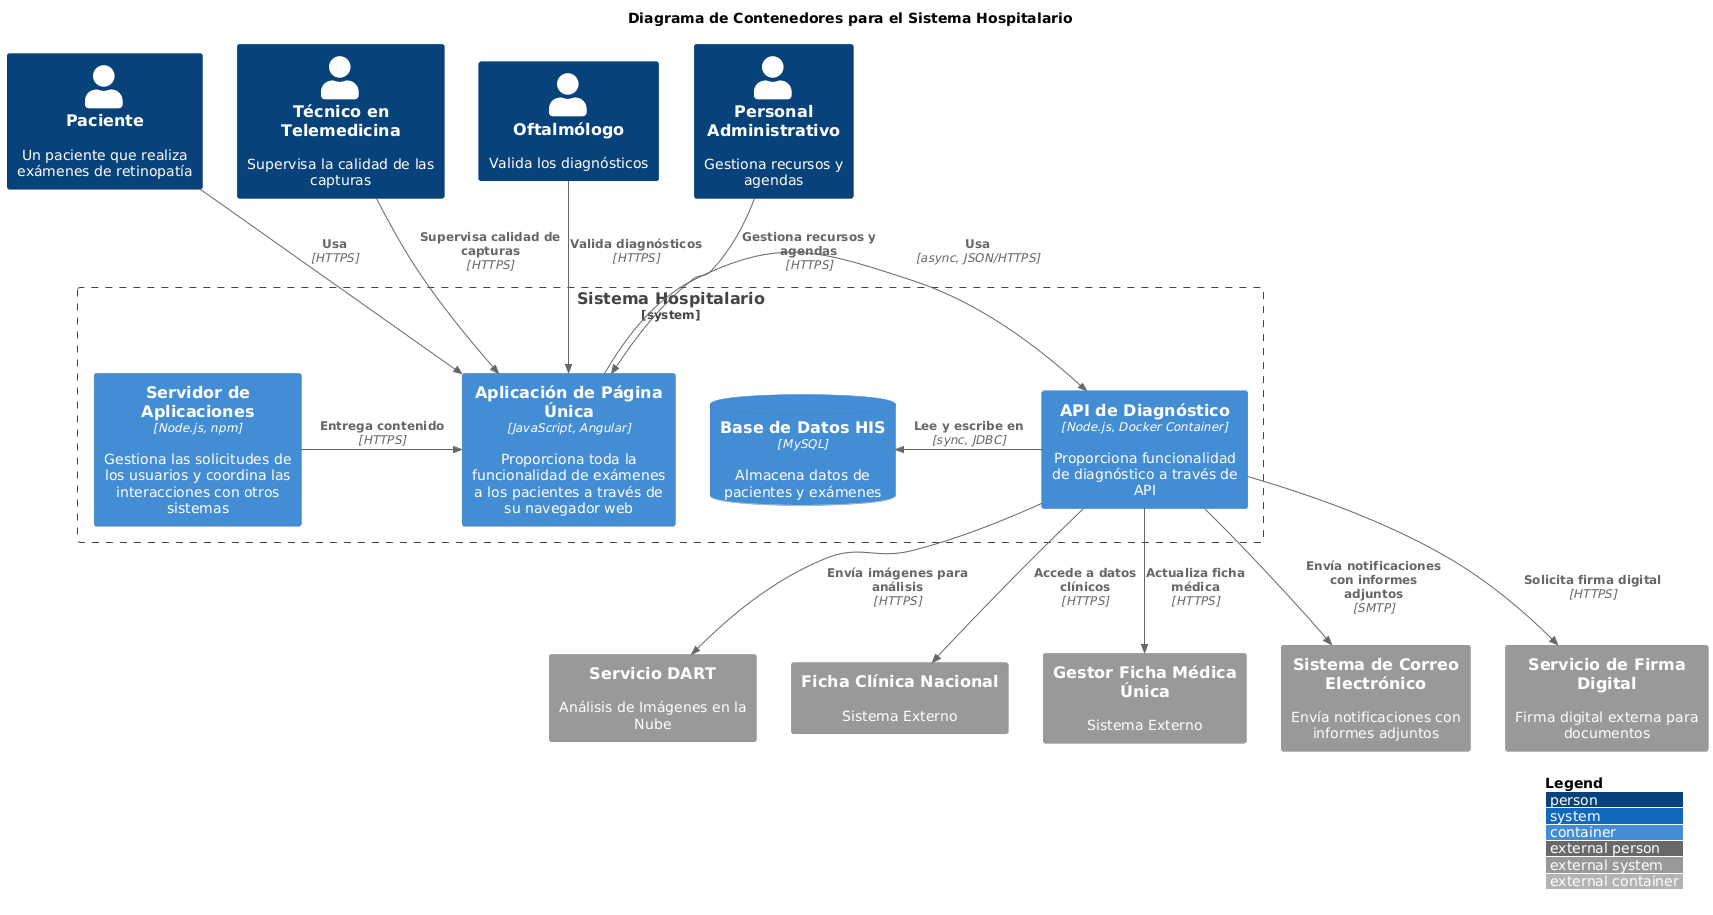
\includegraphics[width=\textwidth]{Pictures/container_diagram.png}
    \caption{Diagrama de Contenedores del Sistema Hospitalario}
    \label{fig:container_diagram}
\end{figure}










\subsubsection{Diagrama de Componentes - Explicación de los Componentes}

\begin{itemize}
    \item \textbf{Componente de Autenticación}: Gestiona la autenticación de usuarios, asegurando que solo usuarios autorizados puedan acceder al sistema.
    \item \textbf{Controlador de Exámenes}: Se encarga de la gestión de exámenes, incluyendo la creación y seguimiento de los mismos.
    \item \textbf{Generador de Informes}: Genera informes de diagnóstico que pueden ser revisados por los médicos y enviados a los pacientes.
    \item \textbf{Integración con DART}: Facilita la comunicación con el servicio DART para el análisis de imágenes.
\end{itemize}

Este diagrama detalla cómo los diferentes módulos dentro de los contenedores interactúan para proporcionar las funcionalidades del sistema. La modularidad de los componentes permite una fácil actualización y mantenimiento del sistema, mientras que la reutilización de componentes comunes mejora la eficiencia del desarrollo.


    \begin{verbatim}
    @startuml
    !include https://raw.githubusercontent.com/plantuml-stdlib/C4-PlantUML/master/C4_Component.puml

    LAYOUT_WITH_LEGEND()

    title Diagrama de Componentes para el Sistema Hospitalario

    Container(spa, "Aplicación de Página Única", "JavaScript y Angular", "Proporciona toda la funcionalidad de exámenes a los pacientes a través de su navegador web.")
    ContainerDb(base_datos_his, "Base de Datos HIS", "MySQL", "Almacena datos de pacientes y exámenes.")
    System_Ext(servicio_dart, "Servicio DART", "Análisis de Imágenes en la Nube")

    Container_Boundary(backend_api, "API de Diagnóstico") {
        Component(auth, "Componente de Autenticación", "Node.js Module", "Gestiona la autenticación de usuarios.")
        Component(exam, "Controlador de Exámenes", "Node.js Module", "Gestiona la creación y seguimiento de exámenes.")
        Component(report, "Generador de Informes", "Node.js Module", "Genera informes de diagnóstico para los pacientes.")
        Component(integration, "Integración con DART", "Node.js Module", "Facilita la comunicación con el servicio DART.")
        
        Rel(auth, base_datos_his, "Lee y escribe en", "JDBC")
        Rel(exam, base_datos_his, "Lee y escribe en", "JDBC")
        Rel(report, base_datos_his, "Lee y escribe en", "JDBC")
        Rel(integration, servicio_dart, "Envía imágenes para análisis", "HTTPS")
    }

    Rel(spa, auth, "Usa", "JSON/HTTPS")
    Rel(spa, exam, "Usa", "JSON/HTTPS")
    Rel(spa, report, "Usa", "JSON/HTTPS")

    @enduml
    \end{verbatim}
\end{itemize}
    \begin{figure}[h]
        \centering
        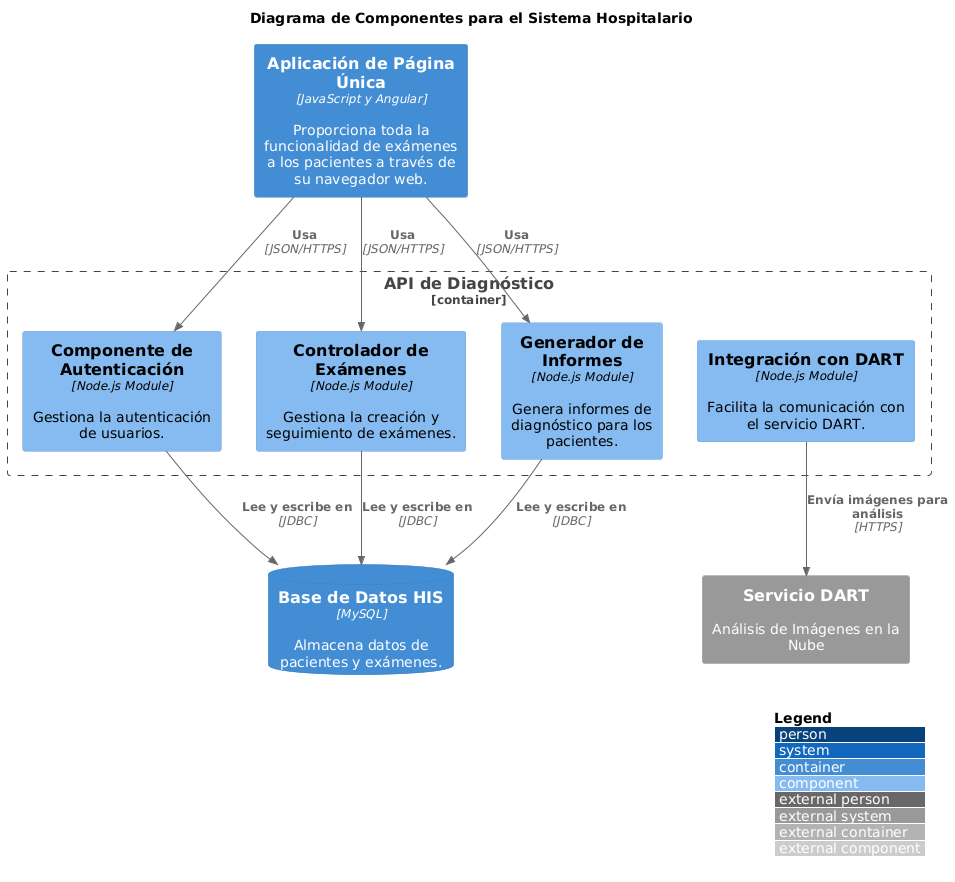
\includegraphics[width=\textwidth]{Pictures/component_diagram.png}
        \caption{Diagrama de Componentes del Sistema Hospitalario}
        \label{fig:component_diagram}
    \end{figure}























%%%%%%%%%%%%%%%%%%%%%%%%%%%%%%%%%%%%%%%%%%%%%%%%%%%
%%%%%%%%%%%%%%%%%%%%%%%%%%%%%%%%%%%%%%%%%%%%%%%%%%%
%%%%%%%%%%%%%%%%%%%%%%%%%%%%%%%%%%%%%%%%%%%%%%%%%%%
%%%%%%%%%%%%%%%%%%%%%%%%%%%%%%%%%%%%%%%%%%%%%%%%%%%
%%%%%%%%%%%%%%%%%%%%%%%%%%%%%%%%%%%%%%%%%%%%%%%%%%%
%%%%%%%%%%%%%%%%%%%%%%%%%%%%%%%%%%%%%%%%%%%%%%%%%%%
\begin{comment}
\section{Evaluación ATAM del Sistema Hospitalario con DART}

Para evaluar la arquitectura propuesta para el sistema DART, aplicaremos el método ATAM (Architecture Tradeoff Analysis Method). Este método nos permitirá analizar cómo los componentes lógicos identificados satisfacen los atributos de calidad requeridos.

\subsection{Identificación de Atributos de Calidad}

Los principales atributos de calidad para el sistema DART son:

\begin{itemize}
    \item \textbf{Desempeño}:
        \begin{itemize}
            \item Tiempo de respuesta del diagnóstico < 5 días
            \item Procesamiento de imágenes en < 1 minuto
            \item Capacidad de procesar 1000 imágenes/día
        \end{itemize}
    \item \textbf{Precisión}:
        \begin{itemize}
            \item Sensibilidad > 90\% en detección de patologías
            \item Especificidad > 85\% en clasificación
            \item Tasa de falsos positivos < 5\%
        \end{itemize}
    \item \textbf{Disponibilidad}:
        \begin{itemize}
            \item Sistema disponible 24/7
            \item Tiempo de inactividad < 1 hora/mes
            \item Recuperación automática de fallos
        \end{itemize}
    \item \textbf{Seguridad}:
        \begin{itemize}
            \item Cumplimiento de la Ley 20.584 (Derechos del Paciente)
            \item Encriptación de datos sensibles
            \item Trazabilidad completa de accesos
        \end{itemize}
\end{itemize}

\subsection{Escenarios de Atributos de Calidad}

Desarrollamos escenarios detallados para cada atributo de calidad:

\subsubsection{Escenario de Desempeño}
\begin{itemize}
    \item \textbf{Estímulo:} Llegada de 100 nuevas imágenes
    \item \textbf{Fuente:} Centro de salud rural
    \item \textbf{Artefacto:} Sistema DART completo
    \item \textbf{Entorno:} Operación normal
    \item \textbf{Respuesta:} Procesamiento y diagnóstico preliminar
    \item \textbf{Medida:} Completado en < 2 horas
\end{itemize}

\subsubsection{Escenario de Precisión}
\begin{itemize}
    \item \textbf{Estímulo:} Imagen con retinopatía moderada
    \item \textbf{Fuente:} Cámara retinal calibrada
    \item \textbf{Artefacto:} Motor de Diagnóstico IA
    \item \textbf{Entorno:} Carga normal del sistema
    \item \textbf{Respuesta:} Clasificación correcta de severidad
    \item \textbf{Medida:} Concordancia > 90\% con oftalmólogo
\end{itemize}

\subsection{Contextualización de Escenarios con 'Ilities'}

Cada escenario del sistema DART se cruza con las características de calidad relevantes, asegurando que se cumplan los objetivos de negocio:

\begin{itemize}
    \item \textbf{Escenario de Desempeño:} Procesamiento de 100 imágenes en menos de 2 horas.
    \begin{itemize}
        \item \textbf{Ilities:} Desempeño, Disponibilidad
    \end{itemize}
    \item \textbf{Escenario de Precisión:} Clasificación correcta de imágenes con retinopatía moderada.
    \begin{itemize}
        \item \textbf{Ilities:} Precisión, Seguridad
    \end{itemize}
\end{itemize}

\subsection{Análisis de Compensaciones}

Los componentes lógicos identificados presentan las siguientes compensaciones:

\begin{enumerate}
    \item \textbf{Componente de Preprocesamiento}:
        \begin{itemize}
            \item \textbf{Beneficio:} Mejora la precisión del diagnóstico
            \item \textbf{Costo:} Aumenta el tiempo de procesamiento
            \item \textbf{Riesgo:} Posible cuello de botella en alta demanda
        \end{itemize}
    
    \item \textbf{Motor de Diagnóstico IA}:
        \begin{itemize}
            \item \textbf{Beneficio:} Automatización y velocidad
            \item \textbf{Costo:} Alta complejidad de mantenimiento
            \item \textbf{Riesgo:} Dependencia de calidad de datos
        \end{itemize}
    
    \item \textbf{Sistema de Validación Médica}:
        \begin{itemize}
            \item \textbf{Beneficio:} Mayor precisión y confiabilidad
            \item \textbf{Costo:} Tiempo adicional en el proceso
            \item \textbf{Riesgo:} Disponibilidad de especialistas
        \end{itemize}
\end{enumerate}

\subsection{Análisis de Riesgos y No-Riesgos}

\subsubsection{Riesgos Arquitectónicos}
\begin{itemize}
    \item \textbf{R1:} Alto acoplamiento del Motor de IA podría dificultar actualizaciones
    \item \textbf{R2:} Dependencia de la calidad de imagen inicial
    \item \textbf{R3:} Posible degradación del rendimiento en horas pico
\end{itemize}

\subsubsection{No-Riesgos}
\begin{itemize}
    \item \textbf{NR1:} Escalabilidad del almacenamiento (uso de cloud)
    \item \textbf{NR2:} Integración con sistemas hospitalarios (APIs estándar)
    \item \textbf{NR3:} Seguridad de datos (encriptación end-to-end)
\end{itemize}

\subsection{Puntos de Sensibilidad y Compensación}

\begin{itemize}
    \item \textbf{S1:} Calidad del preprocesamiento vs. tiempo de respuesta
    \item \textbf{S2:} Automatización vs. precisión del diagnóstico
    \item \textbf{S3:} Disponibilidad vs. costos de infraestructura
\end{itemize}

\subsection{Recomendaciones Arquitectónicas}

Basados en el análisis ATAM, recomendamos:

\begin{enumerate}
    \item Implementar procesamiento por lotes para optimizar rendimiento
    \item Desarrollar un sistema de caché para resultados frecuentes
    \item Establecer un pipeline de validación automática de imágenes
    \item Implementar monitoreo continuo de precisión del modelo
    \item Diseñar un sistema de retroalimentación para mejora continua
\end{enumerate}

\section{Arquitectura del Sistema Hospitalario con DART}

\subsection{Vista de Componentes Lógicos}

La siguiente figura muestra la arquitectura de componentes lógicos del sistema hospitalario que integra DART:

\begin{figure}[h]
\begin{verbatim}
@startuml
package "Sistema Hospitalario" {
    package "DART" {
        [Adquisición de Imágenes] as AI
        [Preprocesamiento] as PP
        [Motor IA] as IA
        [Validación Médica] as VM
        [Gestor de Derivaciones] as GD
    }
    
    package "HIS (Sistema de Información Hospitalaria)" {
        [Gestión de Pacientes] as GP
        [Agenda Médica] as AM
        [Historia Clínica] as HC
        [Farmacia] as FA
    }
    
    package "Telemedicina" {
        [Portal Médico] as PM
        [Portal Paciente] as PP2
        [Gestor de Teleconsultas] as GT
    }
    
    database "Almacenamiento" {
        [Base de Datos Clínica] as BDC
        [Repositorio de Imágenes] as RI
        [Base de Conocimiento IA] as BCIA
    }
}

' Relaciones DART
AI --> PP : imágenes
PP --> IA : imágenes preprocesadas
IA --> VM : diagnóstico preliminar
VM --> GD : decisión derivación
AI --> RI : almacena
IA --> BCIA : consulta/actualiza

' Relaciones HIS
GP --> HC : actualiza
AM --> HC : registra
FA --> HC : prescripciones
HC --> BDC : almacena

' Integraciones
GP --> AI : datos paciente
VM --> HC : diagnóstico final
GD --> AM : agenda derivación
PM --> VM : acceso remoto
GT --> VM : teleconsulta
PP2 --> HC : consulta

@enduml
\end{verbatim}
\caption{Arquitectura de Componentes Lógicos del Sistema Hospitalario con DART}
\label{fig:arch_components}
\end{figure}

\subsection{Descripción de Componentes}

Los componentes se organizan en cuatro paquetes principales:

\subsubsection{DART}
\begin{itemize}
    \item \textbf{Adquisición de Imágenes}: Captura y validación inicial de imágenes retinales
    \item \textbf{Preprocesamiento}: Normalización y mejora de imágenes
    \item \textbf{Motor IA}: Análisis automatizado y detección de patologías
    \item \textbf{Validación Médica}: Interfaz para revisión y confirmación por especialistas
    \item \textbf{Gestor de Derivaciones}: Coordinación de referencias a especialistas
\end{itemize}

\subsubsection{HIS (Sistema de Información Hospitalaria)}
\begin{itemize}
    \item \textbf{Gestión de Pacientes}: Registro y administración de datos demográficos
    \item \textbf{Agenda Médica}: Programación de citas y recursos médicos
    \item \textbf{Historia Clínica}: Registro centralizado de información clínica
    \item \textbf{Farmacia}: Gestión de medicamentos y prescripciones
\end{itemize}

\subsubsection{Telemedicina}
\begin{itemize}
    \item \textbf{Portal Médico}: Acceso remoto para profesionales de salud
    \item \textbf{Portal Paciente}: Interfaz de autoservicio para pacientes
    \item \textbf{Gestor de Teleconsultas}: Coordinación de consultas remotas
\end{itemize}

\subsubsection{Almacenamiento}
\begin{itemize}
    \item \textbf{Base de Datos Clínica}: Almacenamiento estructurado de datos clínicos
    \item \textbf{Repositorio de Imágenes}: Almacenamiento especializado para imágenes médicas
    \item \textbf{Base de Conocimiento IA}: Modelos y datos de entrenamiento
\end{itemize}

\subsection{Patrones de Integración}

El diagrama muestra varios patrones de integración importantes:

\begin{enumerate}
    \item \textbf{Flujo de Trabajo DART}:
        \begin{itemize}
            \item Secuencia lineal de procesamiento de imágenes
            \item Puntos de decisión en validación médica
            \item Retroalimentación para mejora continua del modelo
        \end{itemize}
    
    \item \textbf{Integración con HIS}:
        \begin{itemize}
            \item Datos demográficos alimentan el proceso DART
            \item Resultados se incorporan a la historia clínica
            \item Derivaciones se coordinan con agenda médica
        \end{itemize}
    
    \item \textbf{Capacidades de Telemedicina}:
        \begin{itemize}
            \item Acceso remoto a diagnósticos
            \item Consultas virtuales de seguimiento
            \item Portal de autoservicio para pacientes
        \end{itemize}
\end{enumerate}

\section{Diagrama de Despliegue del Sistema Hospitalario con DART}

\subsection{Vista de Despliegue}

La siguiente figura muestra el diagrama de despliegue del sistema hospitalario que integra DART, reflejando el proceso completo:

\begin{figure}[h]
\begin{verbatim}
@startuml
node "Usuario" {
    [PC del Usuario] --> [Cámara Retinal]
}

node "Red Hospitalaria" {
    node "Servidor DART" {
        [Consulta Recibida] --> [Preprocesar Imágenes]
        [Preprocesar Imágenes] --> [Detectar Signos de Retinopatía]
        [Detectar Signos de Retinopatía] --> [Generar Propuesta de Reporte]
        [Generar Propuesta de Reporte] --> [Validación Profesional]
        [Validación Profesional] --> [Notificar Paciente]
        [Validación Profesional] --> [Petición de Intervención]
    }
    
    node "Base de Datos" {
        [Repositorio de Imágenes]
        [Base de Conocimiento IA]
    }
}

node "Interfaz de Telemedicina" {
    [Portal Médico]
    [Portal Paciente]
}

' Conexiones
[PC del Usuario] --> [Consulta Recibida] : Captura
[Generar Propuesta de Reporte] --> [Repositorio de Imágenes] : Almacenamiento
[Detectar Signos de Retinopatía] --> [Base de Conocimiento IA] : Consulta
[Validación Profesional] --> [Portal Médico] : Resultados
[Portal Paciente] --> [Validación Profesional] : Consulta

@enduml
\end{verbatim}
\caption{Diagrama de Despliegue del Sistema Hospitalario con DART}
\label{fig:deployment_diagram}
\end{figure}























\section{Evaluación de la Arquitectura}

La evaluación de la arquitectura se realiza utilizando métodos como el ATAM para asegurar que los componentes lógicos identificados satisfacen los atributos de calidad requeridos.

\begin{itemize}
    \item \textbf{ATAM (Architecture Tradeoff Analysis Method)}: Método utilizado para analizar cómo los componentes lógicos satisfacen los atributos de calidad.
    \item \textbf{Identificación de Atributos de Calidad}: Evaluar atributos como desempeño, precisión, disponibilidad y seguridad.
    \item \textbf{Escenarios de Atributos de Calidad}: Desarrollar escenarios detallados para cada atributo de calidad.
    \item \textbf{Análisis de Compensaciones}: Identificar beneficios, costos y riesgos de los componentes lógicos.
    \item \textbf{Recomendaciones Arquitectónicas}: Proponer mejoras basadas en el análisis ATAM.
\end{itemize}

\textbf{Workshop ATAM para el Piloto del Sistema DART en un Hospital}

Este workshop está diseñado para simular una evaluación ATAM en un hospital donde se implementará un piloto del sistema DART, solicitado por el Ministerio de Salud. Los participantes incluirán personal del hospital, arquitectos del sistema, y otros stakeholders relevantes.
\subsection{Objetivos del Workshop}
\begin{itemize}
    \item Evaluar la arquitectura del sistema DART en el contexto del hospital.
    \item Identificar riesgos y oportunidades de mejora.
    \item Fomentar la comunicación entre los stakeholders.
\end{itemize}

\subsection{Roles y Responsabilidades}
\begin{itemize}
    \item \textbf{Líder de Evaluación}: Facilita el proceso del workshop.
    \item \textbf{Portavoz del Proyecto}: Representante del hospital que presenta los objetivos de negocio.
    \item \textbf{Arquitecto del Sistema}: Presenta la arquitectura del sistema DART.
    \item \textbf{Stakeholders}: Incluyen médicos, personal técnico, y representantes del ministerio.
\end{itemize}

\subsection{Materiales del Workshop}
\begin{itemize}
    \item \textbf{Presentación de Diapositivas}: Guía visual para el workshop.
        \begin{itemize}
            \item \textbf{Código en Gamma para generar diapositivas}:
            \begin{verbatim}
            slide "Introducción al ATAM" {
                title: "Introducción al ATAM"
                content: "Presentación interactiva sobre el método ATAM."
            }

            slide "Presentación de Impulsores de Negocio" {
                title: "Presentación de Impulsores de Negocio"
                content: "Discusión liderada por el portavoz del proyecto."
            }

            slide "Presentación de la Arquitectura" {
                title: "Presentación de la Arquitectura"
                content: "Exposición del arquitecto del sistema."
            }

            slide "Generación del Árbol de Utilidad" {
                title: "Generación del Árbol de Utilidad"
                content: "Taller colaborativo para identificar atributos de calidad."
            }

            slide "Análisis de Enfoques Arquitectónicos" {
                title: "Análisis de Enfoques Arquitectónicos"
                content: "Evaluación de enfoques mediante discusión grupal."
            }

            slide "Lluvia de Ideas y Priorización de Escenarios" {
                title: "Lluvia de Ideas y Priorización de Escenarios"
                content: "Sesión de brainstorming con votación para priorizar escenarios."
            }

            slide "Análisis de Enfoques Arquitectónicos (Reiteración)" {
                title: "Análisis de Enfoques Arquitectónicos (Reiteración)"
                content: "Revisión de escenarios priorizados y análisis detallado."
            }

            slide "Presentación de Resultados" {
                title: "Presentación de Resultados"
                content: "Presentación final de hallazgos y recomendaciones."
            }
            \end{verbatim}
        \end{itemize}
    
    
        
    
    \item \textbf{Documentación de la Arquitectura}: Descripciones detalladas del sistema DART.
\end{itemize}

\subsection{Emulación del Workshop y Resultados Esperados}

Durante el workshop, los alumnos emularán cada paso del ATAM para obtener resultados específicos. A continuación, se describe la dinámica de cada paso, los modelos o detalles arquitectónicos presentados, y los resultados esperados, resaltados en azul.

\begin{enumerate}
    \item \textbf{Introducción al ATAM}
    \begin{itemize}
        \item \textit{Alumno (Presentador)}: Debe realizar una presentación interactiva sobre el método ATAM.
        \begin{itemize}
            \item \textcolor{blue}{Introducción al método ATAM.}
            \item \textcolor{blue}{Explicación de los pasos del proceso.}
            \item \textcolor{blue}{Importancia del método en la arquitectura de software.}
        \end{itemize}
        \item \textit{Modelo/Detalles}: Se muestra un diagrama general del proceso ATAM.
        \item \textit{Resultado}: \textcolor{blue}{Comprensión clara del método ATAM y su importancia.}
    \end{itemize}

    \item \textbf{Presentación de Impulsores de Negocio}
    \begin{itemize}
        \item \textit{Dinámica}: Discusión liderada por el portavoz del proyecto.
        \item \textit{Modelo/Detalles}: Se presentan los objetivos del Hospital 2.0, que incluyen mejorar la accesibilidad a servicios de salud, aumentar la eficiencia operativa y garantizar diagnósticos precisos y oportunos. Estos objetivos influyen en la arquitectura del servicio de diagnóstico remoto de retinopatía diabética al requerir una infraestructura tecnológica robusta, integración con sistemas existentes y un enfoque centrado en el paciente.
        \item \textit{Resultado}: \textcolor{blue}{Identificación de los impulsores arquitectónicos clave para el Hospital 2.0, tales como la mejora de la accesibilidad a servicios de salud, el aumento de la eficiencia operativa y la garantía de diagnósticos precisos y oportunos, asegurando que la arquitectura soporte los objetivos estratégicos del hospital.}
    \end{itemize}



    
    \item \textbf{Presentación de la Arquitectura}
    \begin{itemize}
        \item \textit{Dinámica}: Exposición del arquitecto del sistema.
        \item \textit{Modelo/Detalles}: Descripción detallada de la arquitectura del sistema DART, incluyendo la vista lógica y la vista física. La vista lógica muestra cómo los componentes funcionales del sistema interactúan, mientras que la vista física ilustra la infraestructura tecnológica subyacente, referenciando las figuras \ref{fig:arch_components} y \ref{fig:deployment_diagram}.
        \item \textit{Resultado}: \textcolor{blue}{Entendimiento de cómo la arquitectura soporta los objetivos de negocio. La arquitectura del sistema DART está diseñada para mejorar la accesibilidad a los servicios de salud mediante la integración con sistemas hospitalarios existentes y la provisión de diagnósticos precisos y oportunos. La vista lógica muestra cómo los componentes funcionales del sistema, como la Gestión de Pacientes y el Motor IA, interactúan para procesar y analizar imágenes médicas. La vista física ilustra la infraestructura tecnológica subyacente, incluyendo bases de datos y servidores, que asegura la disponibilidad y escalabilidad del sistema.}
    \end{itemize}

    \item \textbf{Construcción del Árbol de Utilidad}
    \begin{itemize}
        \item \textit{Dinámica}: Durante el ATAM, se lleva a cabo un taller colaborativo dirigido por el arquitecto del sistema, con la participación de todos los stakeholders clave. Se inicia con una discusión para identificar y priorizar los atributos de calidad, construyendo un árbol de utilidad que prioriza el impacto de cada atributo en los objetivos de negocio.
        \item \textit{Modelo/Detalles}: A continuación se presenta un árbol de utilidad, donde los atributos de calidad se organizan jerárquicamente según su impacto. Este esquema incluye ejemplos específicos para DART, destacando el atributo de Desempeño como prioritario.

      



        \item \textit{Resultado}: \textcolor{blue}{Clarificación de los atributos de calidad críticos, priorizando aquellos con mayor impacto en los objetivos del sistema, asegurando una comprensión común entre todos los participantes.}
    \end{itemize}

    \begin{itemize}
        \item \textbf{Desempeño}
        \begin{itemize}
            \item Latencia (H,H): Procesamiento de imágenes en menos de 1 minuto.
            \item Carga máxima (H,M): Respuesta del sistema en tiempo real.
        \end{itemize}
        \item \textbf{Disponibilidad}
        \begin{itemize}
            \item Tiempo de actividad (H,H): Sistema disponible 99.9% del tiempo.
            \item Fallo de software (M,M): Recuperación en menos de 30 segundos.
        \end{itemize}
        \item \textbf{Precisión}
        \begin{itemize}
            \item Sensibilidad (H,L): Sensibilidad > 90%.
            \item Especificidad (H,L): Especificidad > 85%.
        \end{itemize}
        \item \textbf{Seguridad}
        \begin{itemize}
            \item Encriptación (H,L): Encriptación de datos.
            \item Trazabilidad (H,L): Trazabilidad de accesos.
        \end{itemize}
        \item \textbf{Escalabilidad}
        \begin{itemize}
            \item Capacidad de usuarios (L,M): Manejo de aumento en el volumen de usuarios.
        \end{itemize}
    \end{itemize}

    \item \textbf{Análisis de Enfoques Arquitectónicos}
    \begin{itemize}
        \item \textit{Enfoque Arquitectónico}: Un enfoque arquitectónico aquí se refiere a la estrategia o método utilizado para estructurar y organizar los componentes del sistema DART, asegurando que cumpla con los requisitos de calidad y funcionalidad.
        \item \textit{Riesgos en Diagramas/Arquitecturas}: Los riesgos pueden incluir problemas como el alto acoplamiento entre componentes, lo que podría dificultar las actualizaciones o la escalabilidad del sistema.
        \item \textit{Puntos de Sensibilidad}: Estos son aspectos críticos del sistema donde pequeños cambios pueden tener un gran impacto, como la relación entre la calidad del preprocesamiento de imágenes y el tiempo de respuesta del sistema.
        \item \textit{Input para el Proceso}: Diagramas de componentes y flujos de datos del sistema DART.
        \item \textit{Salida del Proceso}: Plantillas que documentan los riesgos identificados y los puntos de sensibilidad.
        \item \textit{Ejemplo en DART}:
        \begin{itemize}
            \item \textbf{Riesgo}: Dependencia excesiva del Motor IA en la calidad de las imágenes preprocesadas podría afectar la precisión del diagnóstico.
            \item \textbf{Punto de Sensibilidad}: Equilibrio entre la automatización del diagnóstico y la precisión requerida.
        \end{itemize}
        \item \textit{Resultado}:
        \begin{itemize}
            \item \textbf{Riesgos Identificados}:
            \begin{itemize}
                \item \textbf{Riesgo 1}: Dependencia excesiva del Motor IA en la calidad de las imágenes preprocesadas.
                \item \textbf{Riesgo 2}: Alto acoplamiento entre componentes que podría dificultar actualizaciones.
            \end{itemize}
            \item \textbf{Puntos de Sensibilidad}:
            \begin{itemize}
                \item \textbf{Punto de Sensibilidad 1}: Equilibrio entre la automatización del diagnóstico y la precisión requerida.
                \item \textbf{Punto de Sensibilidad 2}: Relación entre la calidad del preprocesamiento de imágenes y el tiempo de respuesta del sistema.
            \end{itemize}
        \end{itemize}
    \end{itemize}

    \item \textbf{Lluvia de Ideas y Priorización de Escenarios}
    \begin{itemize}
        \item \textit{Dinámica}: Sesión de brainstorming con votación para priorizar escenarios.
        \item \textit{Modelo/Detalles}: Listado de escenarios y su impacto en la arquitectura, utilizando los modelos C4.
        \item \textit{Ejemplos de Escenarios}:
        \begin{itemize}
            \item \textbf{Escenario 1}: Integración del Sistema DART con el Sistema de Información Hospitalaria para la transferencia de datos de pacientes.
            \item \textbf{Escenario 2}: Escalabilidad del Sistema DART para manejar un aumento en el volumen de usuarios durante campañas de salud pública.
            \item \textbf{Escenario 3}: Implementación de medidas de seguridad para proteger los datos de los pacientes en el Sistema DART.
            \item \textbf{Escenario 4}: Optimización del tiempo de respuesta del Motor de Diagnóstico IA bajo diferentes condiciones de carga.
        \end{itemize}
        \item \textit{Resultado}: \textcolor{blue}{Priorización de escenarios críticos para el análisis, asegurando que estén alineados con los modelos C4.}
    \end{itemize}

    \item \textbf{Análisis de Enfoques Arquitectónicos (Reiteración)}
    \begin{itemize}
        \item \textit{Dinámica}: Revisión de escenarios priorizados y análisis detallado.
        \item \textit{Modelo/Detalles}: Revisión de diagramas y modelos de arquitectura.
        \item \textit{Resultado}: \textcolor{blue}{Identificación de cambios necesarios en la arquitectura para abordar los escenarios. Por ejemplo, se podría descubrir la necesidad de un nuevo componente de seguridad para proteger los datos de los pacientes, lo cual llevaría a modificar la arquitectura existente.}
    \end{itemize}

    \item \textbf{Presentación de Resultados}
    \begin{itemize}
        \item \textit{Dinámica}: Presentación final de hallazgos y recomendaciones.
        \item \textit{Modelo/Detalles}: Resumen visual de los resultados del ATAM.
        \item \textit{Resultado}: \textcolor{blue}{Documentación de riesgos, no-riesgos, y recomendaciones arquitectónicas.}
    \end{itemize}
\end{enumerate}

\subsection{Resultados Esperados}
En conclusión, a lo largo de este curso hemos aprendido los fundamentos del diseño arquitectónico, la importancia de un método sistemático y los conceptos de diseño y drivers arquitectónicos. También hemos estudiado las características de calidad según ISO/IEC 9126 y el proceso de diseño arquitectónico. 

Aplicamos estos conocimientos al sistema DART del MINSAL, identificando componentes lógicos y patrones de acoplamiento, y utilizando el modelo C4 para construir la arquitectura del hospital con DART. Realizamos una evaluación detallada de la arquitectura del sistema en el contexto del hospital, identificando riesgos y oportunidades de mejora, y fomentando la comunicación entre los stakeholders.

Los resultados de nuestro análisis incluyen específicamente la identificación de dos riesgos críticos: la dependencia excesiva del Motor IA en la calidad de las imágenes preprocesadas y el alto acoplamiento entre componentes que podría dificultar actualizaciones. También se identificaron oportunidades de mejora en la escalabilidad del sistema y en la implementación de medidas de seguridad para proteger los datos de los pacientes. Además, se clarificaron los requisitos de calidad, como la precisión del diagnóstico y el tiempo de respuesta del sistema, y se mejoró la documentación de la arquitectura, detallando los componentes y sus interacciones. Estos resultados son esenciales para el éxito del sistema y proporcionan una base sólida para futuras referencias y desarrollos. Además, hemos logrado una comunicación efectiva entre los stakeholders, lo cual es vital para la colaboración y el alineamiento de objetivos.

\end{comment}




\section{Referencias}

\begin{itemize}
    \item Cervantes, H., Kazman, R. (2016). Designing Software Architectures: A Practical Approach, 2nd Edition. Addison-Wesley Professional.
    \item Gandhi, R., Richards, M., Ford, N. (2023). Head First Software Architecture: A Learner's Guide to Architectural Thinking. O'Reilly Media.
\end{itemize}


\input{caps/04-PatronesDiseño}
%\input{caps/100-TrabajoInvestigación}
%\chapterimage{ia.png}
\chapter{Ejercicios}

\section*{Pregunta 1}

\begin{flushright}
   \textit{(- puntos)}
\end{flushright}
%\vspace{20px}


\section{Tipo de preguntas o Ejercicios que debemos resolver al finalizar la asignatura} 
\subsection{Ejercicio 1: Identificación de Alcances}
\textbf{Instrucciones:} Clasifica los siguientes escenarios como parte de la arquitectura empresarial (AE) o de la arquitectura de software (AS). Explica tu elección en cada caso.

\begin{enumerate}
    \item Decidir los estándares de interoperabilidad entre las aplicaciones de diferentes departamentos.
    \item Elegir una estructura de base de datos específica para una aplicación de inventarios.
    \item Diseñar una estrategia para cumplir con regulaciones legales internacionales en todas las aplicaciones corporativas.
    \item Seleccionar un patrón de diseño para la implementación de un sistema de notificaciones.
\end{enumerate}

\subsection{Ejercicio 2: Análisis de Roles}
\textbf{Instrucciones:} Lee las siguientes responsabilidades y asigna si corresponden al arquitecto empresarial (AE) o al arquitecto de aplicaciones (AA). Explica por qué.

\begin{enumerate}
    \item Garantizar que todas las aplicaciones dentro de la organización cumplan con los estándares de seguridad definidos.
    \item Optimizar el rendimiento de un servicio específico utilizado por un equipo de desarrollo.
    \item Definir cómo las aplicaciones de marketing y ventas deben integrarse para compartir datos.
    \item Crear diagramas detallados de componentes y flujos de datos de una aplicación.
\end{enumerate}

\subsection{Ejercicio 3: Diseño de Escenarios}
\textbf{Instrucciones:} Dado un escenario, define las actividades que llevarían a cabo tanto el arquitecto empresarial como el arquitecto de software.

\textbf{Escenario:} Una empresa desea lanzar una nueva plataforma de comercio electrónico, integrada con su sistema de gestión de inventarios existente y cumpliendo con normativas de privacidad de datos en todos los mercados donde opera.

\textbf{Arquitecto Empresarial:}
\begin{enumerate}
    \item Enumera tres actividades clave que realizaría para asegurar que el sistema funcione dentro del ecosistema empresarial.
\end{enumerate}

\textbf{Arquitecto de Software:}
\begin{enumerate}
    \item Detalla tres decisiones técnicas que tomaría para diseñar la arquitectura de la aplicación de comercio electrónico.
\end{enumerate}

%\section{Modelos}
\section{Ciclo iterativo de creación de arquitectura de software}
Cuando un ingeniero se enfrenta con un problema complejo, los ingenieros hacen uso de su capacidad de abstracción.  Claramente los problemas simples pueden resolverse directamente. Sino, mapeamos el problema a un modelo abstracto (por ejemplo una ecuación), resolvemos el problema utilizando el modelo, y luego traducimos esa solución al mundo real.


\begin{flushright}
    \textit{Los modelos y abstracciones son útiles cuando queremos explicar o aprender del sistema. Probablemente más útiles que inspeccionar directamente el código fuente. }
\end{flushright}

%%%%%%


\newpage
\section{¿Por qué evaluar una arquitectura}
Cuanto más temprano se encuentre un problema en un proyecto, menor impacto. Una arquitectura es adecuada cuando el sistema resultante de ella cumple los objetivos de calidad con la meta de mitigar los riesgos. 



\newpage
\section{Control - Caso}


\section{Componentes Lógicos: Los Bloques Fundamentales}

Los componentes lógicos son los bloques funcionales fundamentales de un sistema que describen cómo sus piezas encajan entre sí. En la mayoría de los lenguajes de programación, estos componentes se representan a través de la estructura de directorios del repositorio de código fuente.

Para ilustrar los conceptos de esta sección, continuaremos con nuestro ejemplo del sistema de subastas en línea "Adventurous Auctions" y el sistema DART.

\subsection{Arquitectura Lógica vs Física}

Es fundamental comprender la diferencia entre estos dos tipos de arquitectura:

\begin{itemize}
    \item \textbf{Arquitectura Lógica}: Muestra los bloques funcionales del sistema y sus interacciones (acoplamiento). Por ejemplo, en Adventurous Auctions, incluiría componentes como "Gestión de Subastas" y "Registro de Pujadores".
    \item \textbf{Arquitectura Física}: Muestra elementos como servicios, bases de datos, y protocolos. En nuestro ejemplo, incluiría elementos como "Base de Datos de Usuarios" y "Servidor de Streaming".
\end{itemize}

\subsection{Identificación de Componentes Lógicos}

Existen dos enfoques principales para identificar los componentes lógicos iniciales:

\subsubsection{Enfoque de Flujo de Trabajo}

Este enfoque identifica componentes siguiendo el flujo principal del sistema. Para Adventurous Auctions y DART:

\begin{enumerate}
    \item Usuario se registra \(\rightarrow\) \textbf{Componente de Registro}
    \begin{itemize}
        \item Validar información del usuario
        \item Almacenar datos de tarjeta de crédito
        \item Crear perfil de pujador
    \end{itemize}
    
    \item Usuario busca subastas \(\rightarrow\) \textbf{Componente de Búsqueda}
    \begin{itemize}
        \item Listar subastas activas
        \item Filtrar por categoría
        \item Mostrar detalles de viajes
    \end{itemize}
    
    \item Usuario participa en subasta \(\rightarrow\) \textbf{Componente de Pujas}
    \begin{itemize}
        \item Procesar pujas en tiempo real
        \item Validar montos
        \item Notificar al subastador
    \end{itemize}
\end{enumerate}

\subsubsection{Enfoque Actor/Acción}

Este enfoque comienza identificando los actores principales y sus acciones:

\begin{itemize}
    \item \textbf{Pujador Online}:
        \begin{itemize}
            \item Registrarse \(\rightarrow\) \textbf{Gestión de Usuarios}
            \item Ver subastas \(\rightarrow\) \textbf{Catálogo de Subastas}
            \item Realizar pujas \(\rightarrow\) \textbf{Procesador de Pujas}
        \end{itemize}
    \item \textbf{Subastador}:
        \begin{itemize}
            \item Iniciar subasta \(\rightarrow\) \textbf{Control de Subastas}
            \item Gestionar pujas presenciales \(\rightarrow\) \textbf{Integración de Pujas}
            \item Cerrar subasta \(\rightarrow\) \textbf{Procesamiento de Pagos}
        \end{itemize}
\end{itemize}

\subsection{La Trampa de las Entidades}

Es común caer en la "trampa de las entidades" al identificar componentes lógicos. Por ejemplo, en Adventurous Auctions, podríamos estar tentados a crear componentes como:

\begin{itemize}
    \item \textbf{Gestor de Pujas} (¡Mal!)
    \item \textbf{Administrador de Usuarios} (¡Mal!)
    \item \textbf{Controlador de Subastas} (¡Mal!)
\end{itemize}

Estos nombres son demasiado vagos y suelen convertirse en componentes que hacen demasiadas cosas. En su lugar, deberíamos tener:

\begin{itemize}
    \item \textbf{Procesador de Pujas en Tiempo Real}
    \item \textbf{Registro y Autenticación de Usuarios}
    \item \textbf{Coordinador de Flujo de Subasta}
\end{itemize}

\subsection{Acoplamiento de Componentes}

El acoplamiento entre componentes es crucial para la mantenibilidad del sistema. En Adventurous Auctions identificamos dos tipos principales:

\begin{itemize}
    \item \textbf{Acoplamiento Aferente (CA)}: Por ejemplo, varios componentes dependen del "Procesador de Pujas en Tiempo Real":
        \begin{itemize}
            \item Interfaz de Usuario (para mostrar pujas)
            \item Sistema de Notificaciones (para alertar a ganadores)
            \item Procesador de Pagos (para cobrar al ganador)
        \end{itemize}
    
    \item \textbf{Acoplamiento Eferente (CE)}: El "Procesador de Pujas" depende de:
        \begin{itemize}
            \item Validador de Usuarios
            \item Sistema de Almacenamiento de Pujas
            \item Notificador de Eventos
        \end{itemize}
\end{itemize}

Para reducir el acoplamiento, aplicamos la Ley de Demeter, que establece que los componentes deben tener conocimiento limitado de otros componentes. Por ejemplo, el Procesador de Pujas no necesita saber cómo se realiza el pago, solo necesita notificar que una puja ha ganado.
%\documentclass{article}
\usepackage[utf8]{inputenc}
\usepackage{graphicx}
\usepackage{color}
\begin{document}
\begin{center}
    
\includegraphics[width=0.5\textwidth]{Pictures/logo.png} \\ % Asegúrate de tener el archivo logo.png en el directorio correcto
    \textbf{FACULTAD DE INGENIERÍA Y CIENCIAS} \\ 
    \textbf{UNIVERSIDAD ADOLFO IBÁÑEZ} \\ 

\end{center}
\title{Control \\ Guía de Estudio para el control de la arquitectura de sistemas}
\author{TICS317 Arquitectura de Sistemas \\ Profesores: Romina Torres, Juan Gana, Eliana Vivas \\ Última actualización: 25 de marzo de 2025}
\date{}
\maketitle



\begin{flushleft}
\textbf{Planteamiento del caso:} 
Una empresa de manufactura de componentes electrónicos de alta precisión para la industria automotriz está implementando tecnologías IoT para mejorar sus procesos. La empresa busca: (1) monitorear en tiempo real la calibración de máquinas de precisión, (2) controlar la calidad de los componentes durante el proceso de producción, (3) gestionar el consumo energético de la planta, y (4) predecir mantenimiento de equipos críticos.
\end{flushleft}

\begin{enumerate}
    \item ¿Qué rol desempeña el arquitecto empresarial en el contexto de la arquitectura empresarial?
    \begin{itemize}
        \item A) Controla la funcionalidad de aplicaciones específicas
        \item B) Diseña el ecosistema dentro del cual las aplicaciones contribuyen a la empresa
        \item C) Desarrolla aplicaciones individuales
        \item D) Supervisa la implementación de software
    \end{itemize}

    \item ¿Cuál es uno de los beneficios de implementar una arquitectura empresarial (AE)?
    \begin{itemize}
        \item A) Aumenta la complejidad de los sistemas de información
        \item B) Facilita la colaboración entre equipos
        \item C) Incrementa los costos operativos
        \item D) Reduce la resiliencia organizacional
    \end{itemize}

    \item ¿Qué lenguaje de modelado estándar se utiliza para la arquitectura empresarial?
    \begin{itemize}
        \item A) UML
        \item B) ArchiMate
        \item C) BPMN
        \item D) SysML
    \end{itemize}

    \item ¿Cuál es uno de los dominios principales de la arquitectura empresarial según TOGAF?
    \begin{itemize}
        \item A) Arquitectura de Seguridad
        \item B) Arquitectura de Negocio
        \item C) Arquitectura de Proyectos
        \item D) Arquitectura de Marketing
    \end{itemize}

    \item ¿Qué principio fundamental de la Ingeniería de Software a Gran Escala (VLSE) se describe cuando se menciona la modularidad?
    \begin{itemize}
        \item A) Complejidad
        \item B) Modularidad
        \item C) Centralización
        \item D) Descentralización
    \end{itemize}

    \item ¿Qué propiedad de calidad se está priorizando cuando se menciona que el sistema debe ser capaz de manejar picos de carga extremos sin comprometer el rendimiento?
    \begin{itemize}
        \item A) Seguridad
        \item B) Escalabilidad
        \item C) Flexibilidad
        \item D) Simplicidad
    \end{itemize}

    \item Ejercicio 2: Análisis de Roles. Lee las siguientes responsabilidades y asigna si corresponden al arquitecto empresarial (AE) o al arquitecto de aplicaciones (AA). Explica por qué.
    \begin{enumerate}
        \item Garantizar que todas las aplicaciones dentro de la organización cumplan con los estándares de seguridad definidos.
        \begin{itemize}
            \item A) Arquitecto Empresarial (AE)
            \item B) Arquitecto de Aplicaciones (AA)
        \end{itemize}
        \item Optimizar el rendimiento de un servicio específico utilizado por un equipo de desarrollo.
        \begin{itemize}
            \item A) Arquitecto Empresarial (AE)
            \item B) Arquitecto de Aplicaciones (AA)
        \end{itemize}
        \item Definir cómo las aplicaciones de marketing y ventas deben integrarse para compartir datos.
        \begin{itemize}
            \item A) Arquitecto Empresarial (AE)
            \item B) Arquitecto de Aplicaciones (AA)
        \end{itemize}
        \item Crear diagramas detallados de componentes y flujos de datos de una aplicación.
        \begin{itemize}
            \item A) Arquitecto Empresarial (AE)
            \item B) Arquitecto de Aplicaciones (AA)
        \end{itemize}
    \end{enumerate}

    \item Instrucciones: Dado un escenario, selecciona las actividades que corresponden al arquitecto empresarial.
    
    Escenario: Una empresa desea lanzar una nueva plataforma de comercio electrónico, integrada con su sistema de gestión de inventarios existente y cumpliendo con normativas de privacidad de datos en todos los mercados donde opera.
    
    \begin{itemize}
        \item A) Asegurar la alineación de la nueva plataforma con los objetivos estratégicos de la empresa.
        \item B) Seleccionar el stack tecnológico adecuado para la plataforma de comercio electrónico.
        \item C) Definir las políticas de privacidad de datos que deben cumplirse.
        \item D) Diseñar la arquitectura de la aplicación para asegurar escalabilidad y rendimiento.
        \item E) Coordinar la integración de la plataforma con el sistema de gestión de inventarios.
    \end{itemize}

\end{enumerate}



    \newpage
    \textbf{Contexto:} Una empresa de manufactura está adoptando tecnologías de IoT para optimizar sus procesos de producción y reducir el desperdicio. La empresa de manufactura se dedica a la producción de componentes electrónicos de alta precisión para la industria automotriz. A continuación se presenta un Balanced Scorecard que refleja los objetivos estratégicos de la empresa.
    
    \begin{table}[h!]
    \centering
    \begin{tabular}{|l|l|l|l|l|}
    \hline
    \textbf{Perspectiva} & \textbf{Objetivo Estratégico} & \textbf{KPI} & \textbf{Valor Actual} & \textbf{Meta a 1 Año / 5 Años} \\ \hline
    Financiera & Reducir costos operativos & Costos operativos totales & \$10M & \$9M / \$7M \\ \hline
    Financiera & Aumentar ROI & ROI de IoT & 5\% & 8\% / 15\% \\ \hline
    Cliente & Mejorar satisfacción del cliente & Índice de satisfacción & 75\% & 80\% / 90\% \\ \hline
    Cliente & Aumentar calidad del producto & Tasa de defectos & 3\% & 2.5\% / 1\% \\ \hline
    Procesos Internos & Optimizar producción & Tiempo de ciclo & 10 horas & 8 horas / 5 horas \\ \hline
    Procesos Internos & Reducir desperdicio & Porcentaje de desperdicio & 10\% & 8\% / 5\% \\ \hline
    Aprendizaje & Mejorar competencias & Horas de capacitación & 20 horas/año & 30 horas/año / 50 horas/año \\ \hline
    Aprendizaje & Fomentar innovación & Nuevas tecnologías & 2 tecnologías & 4 tecnologías / 10 tecnologías \\ \hline
    \end{tabular}
    \caption{Balanced Scorecard de la empresa de manufactura}
    \end{table}
    

\section*{Parte 1: Construcción de la Vista Motivacional}

\begin{enumerate}
    \item \textbf{Identificación de Stakeholders:}
    Describe quiénes son los stakeholders clave en el proyecto de adopción de IoT y cuál es su interés específico en el proyecto.
    
    \color{blue}{\textit{Ejemplo de respuesta: Los stakeholders clave incluyen: (1) Director de Operaciones, interesado en la eficiencia operativa y reducción de costos de la planta, (2) Gerente de Producción, responsable de mantener la calidad de los componentes electrónicos y cumplir con estándares automotrices, (3) Equipo de TI, encargado de implementar la infraestructura IoT y asegurar la integración con sistemas existentes, (4) Clientes de la industria automotriz, que requieren componentes de alta precisión y calidad certificada.}}
    
    \begin{table}[h!]
    \centering
    \begin{tabular}{|c|p{10cm}|}
    \hline
    \textbf{Puntaje} & \textbf{Criterio} \\ \hline
    0 & No identifica stakeholders o identifica stakeholders irrelevantes para el contexto. \\ \hline
    1 & Identifica stakeholders relevantes pero no explica su interés específico en el proyecto IoT. \\ \hline
    2 & Identifica correctamente los stakeholders y explica claramente su interés específico en relación con la manufactura de componentes electrónicos. \\ \hline
    \end{tabular}
    \end{table}

    \item \textbf{Definición de Drivers:}
    Enumera los drivers que motivan la adopción de IoT en la empresa y explica cómo se relacionan con las necesidades específicas de la industria automotriz.
    
    \color{blue}{\textit{Ejemplo de respuesta: Los drivers incluyen: (1) Eficiencia Operativa, para mantener la precisión en la calibración de máquinas y reducir tiempos de inactividad, (2) Reducción de Costos, mediante la optimización del consumo energético y mantenimiento predictivo, (3) Sostenibilidad, para cumplir con regulaciones ambientales de la industria automotriz, (4) Calidad del Producto, para mantener la tasa de defectos por debajo del 3\% requerido por los clientes automotrices.}}
    
    \begin{table}[h!]
    \centering
    \begin{tabular}{|c|p{10cm}|}
    \hline
    \textbf{Puntaje} & \textbf{Criterio} \\ \hline
    0 & No enumera drivers o los drivers no están relacionados con la industria. \\ \hline
    1 & Enumera drivers generales sin vincularlos a las necesidades específicas de la manufactura de componentes electrónicos. \\ \hline
    2 & Enumera drivers relevantes y los vincula claramente con las necesidades específicas de la industria automotriz. \\ \hline
    \end{tabular}
    \end{table}

    \item \textbf{Establecimiento de Objetivos:}
    Define los objetivos estratégicos específicos que la empresa busca alcanzar con la implementación de IoT.
    
    \color{blue}{\textit{Ejemplo de respuesta: Los objetivos incluyen: (1) Reducir la tasa de defectos al 1\% mediante monitoreo en tiempo real de la calibración, (2) Disminuir el consumo energético en un 20\% a través de la gestión inteligente de la planta, (3) Implementar mantenimiento predictivo para reducir el tiempo de inactividad en un 30\%, (4) Alcanzar certificación ISO 9001:2015 para procesos de manufactura con IoT.}}
    
    \begin{table}[h!]
    \centering
    \begin{tabular}{|c|p{10cm}|}
    \hline
    \textbf{Puntaje} & \textbf{Criterio} \\ \hline
    0 & No define objetivos o los objetivos no son medibles. \\ \hline
    1 & Define objetivos generales sin métricas específicas. \\ \hline
    2 & Define objetivos SMART (Específicos, Medibles, Alcanzables, Relevantes y Temporales) alineados con la industria. \\ \hline
    \end{tabular}
    \end{table}

    \item \textbf{Evaluación de Datos del Balance:}
    Describe cómo las evaluaciones (assessments) se relacionan con los objetivos y drivers específicos.
    
    \color{blue}{\textit{Ejemplo de respuesta: Las evaluaciones clave incluyen: (1) Tasa de defectos actual del 3\% que debe reducirse al 1\% para mejorar la calidad del producto, (2) Meta de reducción del tiempo de inactividad en un 30\% para aumentar la eficiencia operativa, (3) Medición del consumo energético actual para establecer metas de reducción que apoyen la sostenibilidad y reducción de costos. Estas evaluaciones están directamente vinculadas con los drivers de Eficiencia Operativa y Sostenibilidad.}}
    
    \begin{table}[h!]
    \centering
    \begin{tabular}{|c|p{10cm}|}
    \hline
    \textbf{Puntaje} & \textbf{Criterio} \\ \hline
    0 & No identifica las evaluaciones específicas o no las relaciona con objetivos/drivers. \\ \hline
    1 & Identifica algunas evaluaciones pero no establece claramente su relación con objetivos y drivers específicos. \\ \hline
    2 & Identifica correctamente las evaluaciones (tasa de defectos, tiempo de inactividad, consumo energético) y las vincula claramente con objetivos y drivers. \\ \hline
    \end{tabular}
    \end{table}

    \item \textbf{Determinación de Outputs:}
    Identifica los outputs técnicos necesarios para alcanzar los objetivos y cómo se relacionan con las evaluaciones.
    
    \color{blue}{\textit{Ejemplo de respuesta: Los outputs incluyen un Plan de Implementación de IoT y un Informe de Evaluación de Impacto, que aseguran el cumplimiento de objetivos estratégicos que les permita lograr consumo energético menor en un 20\%, tiempo de inactividad en un 30\%, Tasa de defectos al 1\%, certificación de manufactura}}
    
    \begin{table}[h!]
    \centering
    \begin{tabular}{|c|p{10cm}|}
    \hline
    \textbf{Puntaje} & \textbf{Criterio} \\ \hline
    0 & No identifica los outputs técnicos o no los relaciona con evaluaciones. \\ \hline
    1 & Identifica algunos outputs pero no establece su relación con evaluaciones específicas. \\ \hline
    2 & Identifica correctamente los cuatro outputs técnicos (monitoreo TR, gestión inteligente, gestión energética, predicción mantenimiento) y los vincula con evaluaciones específicas. \\ \hline
    \end{tabular}
    \end{table}

    \item \textbf{Especificación de Requerimientos:}
    Enumera los requerimientos técnicos necesarios para implementar los outputs identificados y explica cómo soportan las evaluaciones.
    
    \color{blue}{\textit{Ejemplo de respuesta: Los requerimientos técnicos incluyen: (1) sistema de monitoreo en tiempo real de calibración - Sensores de calibración y sistema de monitoreo en tiempo real para control de calidad, (2) sistema de gestión inteligente de planta - Infraestructura IoT y red de sensores para la gestión inteligente de la planta, (3) sistema inteligente de gestión del consumo energético - Medidores inteligentes y sistema de análisis para gestión del consumo energético, (4) sistema de predicción de mantenimiento de equipos críticos - Sensores de condición de equipos y algoritmos predictivos para mantenimiento. Cada requerimiento está diseñado para soportar un output específico y permite alcanzar las metas establecidas en las evaluaciones.}}
    
    \begin{table}[h!]
    \centering
    \begin{tabular}{|c|p{10cm}|}
    \hline
    \textbf{Puntaje} & \textbf{Criterio} \\ \hline
    0 & No especifica requerimientos técnicos o no los relaciona con outputs. \\ \hline
    1 & Especifica algunos requerimientos pero no establece claramente su relación con outputs y evaluaciones. \\ \hline
    2 & Especifica correctamente los requerimientos técnicos y los vincula claramente con outputs y evaluaciones específicas. \\ \hline
    \end{tabular}
    \end{table}

    \item \textbf{Desarrollo de la Vista Motivacional:}
    Dibuja la vista motivacional basada en los elementos identificados anteriormente.
    
    \color{blue}{\textit{Ejemplo de respuesta: Un diagrama que muestra la relación entre stakeholders, drivers, objetivos, assessments, outputs y requerimientos.}}
    
    \begin{table}[h!]
    \centering
    \begin{tabular}{|c|p{10cm}|}
    \hline
    \textbf{Puntaje} & \textbf{Criterio} \\ \hline
    0 & No presenta un diagrama o es incorrecto. \\ \hline
    1 & Presenta un diagrama pero con errores o incompleto. \\ \hline
    2 & Presenta un diagrama correcto y completo. \\ \hline
    \end{tabular}
    \end{table}

\end{enumerate}

\section*{Parte 2: Construcción de la Vista en Capas (Layered View)}

\begin{enumerate}
    \item \textbf{Definición de la Capa de Negocio:}
    Describe los procesos de negocio clave que soportan los objetivos estratégicos de la empresa de manufactura de componentes electrónicos.
    
    \color{blue}{\textit{Ejemplo de respuesta: Los procesos de negocio clave incluyen: (1) Proceso de Calibración de Máquinas de Precisión, que asegura la calidad en la manufactura de componentes, (2) Proceso de Control de Calidad en Línea, que mantiene la tasa de defectos por debajo del 3\%, (3) Proceso de Gestión Energética, que optimiza el consumo de recursos, (4) Proceso de Mantenimiento Predictivo, que reduce tiempos de inactividad. Estos procesos están directamente alineados con los drivers de Eficiencia Operativa y Calidad del Producto.}}
    
    \begin{table}[h!]
    \centering
    \begin{tabular}{|c|p{10cm}|}
    \hline
    \textbf{Puntaje} & \textbf{Criterio} \\ \hline
    0 & No describe procesos de negocio relevantes para la manufactura de componentes electrónicos. \\ \hline
    1 & Describe procesos generales sin vincularlos a los objetivos específicos de calidad y eficiencia. \\ \hline
    2 & Describe correctamente los procesos clave y los vincula con los objetivos de reducción de defectos, eficiencia energética y mantenimiento. \\ \hline
    \end{tabular}
    \end{table}

    \item \textbf{Identificación de Servicios de Negocio:}
    Enumera los servicios de negocio que se ofrecen a los clientes de la industria automotriz y cómo están soportados por los procesos de negocio.
    
    \color{blue}{\textit{Ejemplo de respuesta: Los servicios clave incluyen: (1) Producción de Componentes de Alta Precisión con tasa de defectos menor al 1\%, soportado por los procesos de calibración y control de calidad, (2) Manufactura Sostenible y Eficiente, respaldada por la gestión energética inteligente, (3) Garantía de Continuidad Operativa, asegurada por el mantenimiento predictivo, (4) Certificación de Calidad Automotriz, sustentada por todos los procesos anteriores.}}
    
    \begin{table}[h!]
    \centering
    \begin{tabular}{|c|p{10cm}|}
    \hline
    \textbf{Puntaje} & \textbf{Criterio} \\ \hline
    0 & No enumera servicios relevantes para la industria automotriz. \\ \hline
    1 & Enumera servicios generales sin vincularlos a los procesos específicos de manufactura. \\ \hline
    2 & Enumera correctamente los servicios y los vincula con los procesos de manufactura de precisión. \\ \hline
    \end{tabular}
    \end{table}

    \item \textbf{Desarrollo de la Capa de Aplicación:}
    Identifica las aplicaciones IoT específicas que soportan los procesos de manufactura y describe su función.
    
    \color{blue}{\textit{Ejemplo de respuesta: Las aplicaciones clave incluyen: (1) Sistema de Monitoreo en Tiempo Real (RTMS) para control de calibración, (2) Sistema de Gestión de Calidad (QMS) integrado con sensores IoT, (3) Sistema de Gestión Energética Inteligente (IEMS) para optimización de consumo, (4) Sistema de Mantenimiento Predictivo (PMS) basado en análisis de datos IoT. Cada aplicación está integrada con sensores específicos y proporciona dashboards en tiempo real.}}
    
    \begin{table}[h!]
    \centering
    \begin{tabular}{|c|p{10cm}|}
    \hline
    \textbf{Puntaje} & \textbf{Criterio} \\ \hline
    0 & No identifica aplicaciones IoT relevantes para manufactura. \\ \hline
    1 & Identifica aplicaciones generales sin especificar su función en el contexto IoT. \\ \hline
    2 & Identifica correctamente las aplicaciones IoT y describe su función específica en la manufactura. \\ \hline
    \end{tabular}
    \end{table}

    \item \textbf{Integración de Aplicaciones:}
    Explica cómo las aplicaciones IoT están integradas para soportar la manufactura de precisión.
    
    \color{blue}{\textit{Ejemplo de respuesta: La integración se realiza mediante: (1) Bus de Servicios Empresariales (ESB) que conecta todos los sistemas IoT, (2) APIs RESTful para intercambio de datos en tiempo real entre sistemas, (3) Base de datos Time-Series para almacenamiento de datos de sensores, (4) Sistema de Mensajería para alertas y notificaciones entre sistemas. Esta integración permite el flujo continuo de datos desde los sensores hasta los dashboards de control.}}
    
    \begin{table}[h!]
    \centering
    \begin{tabular}{|c|p{10cm}|}
    \hline
    \textbf{Puntaje} & \textbf{Criterio} \\ \hline
    0 & No explica la integración de sistemas IoT. \\ \hline
    1 & Explica integración general sin especificar mecanismos para datos en tiempo real. \\ \hline
    2 & Explica correctamente la integración de sistemas IoT y el flujo de datos en tiempo real. \\ \hline
    \end{tabular}
    \end{table}

    \item \textbf{Definición de la Capa de Tecnología:}
    Describe la infraestructura tecnológica que soporta las aplicaciones IoT en la planta de manufactura.
    
    \color{blue}{\textit{Ejemplo de respuesta: La infraestructura incluye: (1) Red de sensores industriales IoT conectados mediante protocolos industriales (MQTT, OPC-UA), (2) Gateway IoT para procesamiento en el borde y filtrado de datos, (3) Servidores en la nube para análisis avanzado y almacenamiento, (4) Red industrial segura con segregación entre IT/OT. Esta infraestructura garantiza la recolección y procesamiento confiable de datos de manufactura.}}
    
    \begin{table}[h!]
    \centering
    \begin{tabular}{|c|p{10cm}|}
    \hline
    \textbf{Puntaje} & \textbf{Criterio} \\ \hline
    0 & No describe infraestructura relevante para IoT industrial. \\ \hline
    1 & Describe infraestructura general sin especificaciones para manufactura. \\ \hline
    2 & Describe correctamente la infraestructura IoT específica para manufactura. \\ \hline
    \end{tabular}
    \end{table}

    \item \textbf{Servicios de Infraestructura:}
    Enumera los servicios de infraestructura necesarios para el funcionamiento de las aplicaciones IoT en manufactura.
    
    \color{blue}{\textit{Ejemplo de respuesta: Los servicios incluyen: (1) Servicio de Conectividad Industrial para sensores IoT, (2) Servicio de Procesamiento en el Borde para datos en tiempo real, (3) Servicio de Almacenamiento y Análisis en la Nube, (4) Servicios de Seguridad Industrial incluyendo firewalls industriales y sistemas de detección de intrusiones (IDS). Estos servicios aseguran la operación continua y segura de la infraestructura IoT.}}
    
    \begin{table}[h!]
    \centering
    \begin{tabular}{|c|p{10cm}|}
    \hline
    \textbf{Puntaje} & \textbf{Criterio} \\ \hline
    0 & No enumera servicios relevantes para IoT industrial. \\ \hline
    1 & Enumera servicios generales sin especificaciones para manufactura. \\ \hline
    2 & Enumera correctamente los servicios específicos para IoT en manufactura. \\ \hline
    \end{tabular}
    \end{table}

    \item \textbf{Evaluación de la Seguridad:}
    Describe las medidas de seguridad implementadas para proteger los sistemas IoT en el entorno de manufactura.
    
    \color{blue}{\textit{Ejemplo de respuesta: Las medidas de seguridad incluyen: (1) Segmentación de red IT/OT mediante firewalls industriales, (2) Autenticación y autorización basada en roles para acceso a sistemas IoT, (3) Encriptación de datos en tránsito y en reposo para información de producción, (4) Monitoreo continuo de seguridad mediante SIEM industrial. Estas medidas protegen tanto la propiedad intelectual como la continuidad operativa.}}
    
    \begin{table}[h!]
    \centering
    \begin{tabular}{|c|p{10cm}|}
    \hline
    \textbf{Puntaje} & \textbf{Criterio} \\ \hline
    0 & No describe medidas de seguridad relevantes para IoT industrial. \\ \hline
    1 & Describe medidas generales sin considerar el contexto de manufactura. \\ \hline
    2 & Describe correctamente las medidas de seguridad específicas para IoT en manufactura. \\ \hline
    \end{tabular}
    \end{table}

    \item \textbf{Desarrollo de la Vista en Capas:}
    Dibuja la vista en capas mostrando cómo las capas de negocio, aplicación y tecnología soportan la manufactura de componentes electrónicos con IoT.
    
    \color{blue}{\textit{Ejemplo de respuesta: Un diagrama que muestra la interconexión entre: (1) Capa de Negocio con los procesos de manufactura, (2) Capa de Aplicación con los sistemas IoT, (3) Capa de Tecnología con la infraestructura de sensores y redes industriales. El diagrama debe mostrar cómo estas capas soportan los objetivos de calidad y eficiencia.}}
    
    \begin{table}[h!]
    \centering
    \begin{tabular}{|c|p{10cm}|}
    \hline
    \textbf{Puntaje} & \textbf{Criterio} \\ \hline
    0 & No presenta un diagrama de capas para manufactura IoT. \\ \hline
    1 & Presenta un diagrama incompleto o sin conexiones claras entre capas. \\ \hline
    2 & Presenta un diagrama completo mostrando claramente cómo las capas soportan la manufactura IoT. \\ \hline
    \end{tabular}
    \end{table}

\end{enumerate}

\end{document} 
}

%---------------------------------------------------------------------
%---------------------------------------------------------------------




%----------------------------------------------------------------------------------------
%	References
%----------------------------------------------------------------------------------------

\chapterimage{Pictures/bigdata.png} % Chapter heading image

\bibliographystyle{plain} % Change this to IEEE or Harvard etc.
\bibliography{references}

\end{document}